% Options for packages loaded elsewhere
\PassOptionsToPackage{unicode}{hyperref}
\PassOptionsToPackage{hyphens}{url}
%
\documentclass[
  a4paper,
  headsepline=true,
  open=any]{scrbook}

\usepackage{amsmath,amssymb}
\usepackage{iftex}
\ifPDFTeX
  \usepackage[T1]{fontenc}
  \usepackage[utf8]{inputenc}
  \usepackage{textcomp} % provide euro and other symbols
\else % if luatex or xetex
  \usepackage{unicode-math}
  \defaultfontfeatures{Scale=MatchLowercase}
  \defaultfontfeatures[\rmfamily]{Ligatures=TeX,Scale=1}
\fi
\usepackage{lmodern}
\ifPDFTeX\else  
    % xetex/luatex font selection
\fi
% Use upquote if available, for straight quotes in verbatim environments
\IfFileExists{upquote.sty}{\usepackage{upquote}}{}
\IfFileExists{microtype.sty}{% use microtype if available
  \usepackage[]{microtype}
  \UseMicrotypeSet[protrusion]{basicmath} % disable protrusion for tt fonts
}{}
\makeatletter
\@ifundefined{KOMAClassName}{% if non-KOMA class
  \IfFileExists{parskip.sty}{%
    \usepackage{parskip}
  }{% else
    \setlength{\parindent}{0pt}
    \setlength{\parskip}{6pt plus 2pt minus 1pt}}
}{% if KOMA class
  \KOMAoptions{parskip=half}}
\makeatother
\usepackage{xcolor}
\setlength{\emergencystretch}{3em} % prevent overfull lines
\setcounter{secnumdepth}{5}
% Make \paragraph and \subparagraph free-standing
\ifx\paragraph\undefined\else
  \let\oldparagraph\paragraph
  \renewcommand{\paragraph}[1]{\oldparagraph{#1}\mbox{}}
\fi
\ifx\subparagraph\undefined\else
  \let\oldsubparagraph\subparagraph
  \renewcommand{\subparagraph}[1]{\oldsubparagraph{#1}\mbox{}}
\fi


\providecommand{\tightlist}{%
  \setlength{\itemsep}{0pt}\setlength{\parskip}{0pt}}\usepackage{longtable,booktabs,array}
\usepackage{calc} % for calculating minipage widths
% Correct order of tables after \paragraph or \subparagraph
\usepackage{etoolbox}
\makeatletter
\patchcmd\longtable{\par}{\if@noskipsec\mbox{}\fi\par}{}{}
\makeatother
% Allow footnotes in longtable head/foot
\IfFileExists{footnotehyper.sty}{\usepackage{footnotehyper}}{\usepackage{footnote}}
\makesavenoteenv{longtable}
\usepackage{graphicx}
\makeatletter
\def\maxwidth{\ifdim\Gin@nat@width>\linewidth\linewidth\else\Gin@nat@width\fi}
\def\maxheight{\ifdim\Gin@nat@height>\textheight\textheight\else\Gin@nat@height\fi}
\makeatother
% Scale images if necessary, so that they will not overflow the page
% margins by default, and it is still possible to overwrite the defaults
% using explicit options in \includegraphics[width, height, ...]{}
\setkeys{Gin}{width=\maxwidth,height=\maxheight,keepaspectratio}
% Set default figure placement to htbp
\makeatletter
\def\fps@figure{htbp}
\makeatother
\newlength{\cslhangindent}
\setlength{\cslhangindent}{1.5em}
\newlength{\csllabelwidth}
\setlength{\csllabelwidth}{3em}
\newlength{\cslentryspacingunit} % times entry-spacing
\setlength{\cslentryspacingunit}{\parskip}
\newenvironment{CSLReferences}[2] % #1 hanging-ident, #2 entry spacing
 {% don't indent paragraphs
  \setlength{\parindent}{0pt}
  % turn on hanging indent if param 1 is 1
  \ifodd #1
  \let\oldpar\par
  \def\par{\hangindent=\cslhangindent\oldpar}
  \fi
  % set entry spacing
  \setlength{\parskip}{#2\cslentryspacingunit}
 }%
 {}
\usepackage{calc}
\newcommand{\CSLBlock}[1]{#1\hfill\break}
\newcommand{\CSLLeftMargin}[1]{\parbox[t]{\csllabelwidth}{#1}}
\newcommand{\CSLRightInline}[1]{\parbox[t]{\linewidth - \csllabelwidth}{#1}\break}
\newcommand{\CSLIndent}[1]{\hspace{\cslhangindent}#1}

\usepackage{booktabs}
\usepackage{longtable}
\usepackage{array}
\usepackage{multirow}
\usepackage{wrapfig}
\usepackage{float}
\usepackage{colortbl}
\usepackage{pdflscape}
\usepackage{tabu}
\usepackage{threeparttable}
\usepackage{threeparttablex}
\usepackage[normalem]{ulem}
\usepackage{makecell}
\usepackage{xcolor}
\makeatletter
\makeatother
\makeatletter
\@ifpackageloaded{bookmark}{}{\usepackage{bookmark}}
\makeatother
\makeatletter
\@ifpackageloaded{caption}{}{\usepackage{caption}}
\AtBeginDocument{%
\ifdefined\contentsname
  \renewcommand*\contentsname{Table of contents}
\else
  \newcommand\contentsname{Table of contents}
\fi
\ifdefined\listfigurename
  \renewcommand*\listfigurename{List of Figures}
\else
  \newcommand\listfigurename{List of Figures}
\fi
\ifdefined\listtablename
  \renewcommand*\listtablename{List of Tables}
\else
  \newcommand\listtablename{List of Tables}
\fi
\ifdefined\figurename
  \renewcommand*\figurename{Figure}
\else
  \newcommand\figurename{Figure}
\fi
\ifdefined\tablename
  \renewcommand*\tablename{Table}
\else
  \newcommand\tablename{Table}
\fi
}
\@ifpackageloaded{float}{}{\usepackage{float}}
\floatstyle{ruled}
\@ifundefined{c@chapter}{\newfloat{codelisting}{h}{lop}}{\newfloat{codelisting}{h}{lop}[chapter]}
\floatname{codelisting}{Listing}
\newcommand*\listoflistings{\listof{codelisting}{List of Listings}}
\makeatother
\makeatletter
\@ifpackageloaded{caption}{}{\usepackage{caption}}
\@ifpackageloaded{subcaption}{}{\usepackage{subcaption}}
\makeatother
\makeatletter
\@ifpackageloaded{tcolorbox}{}{\usepackage[skins,breakable]{tcolorbox}}
\makeatother
\makeatletter
\@ifundefined{shadecolor}{\definecolor{shadecolor}{rgb}{.97, .97, .97}}
\makeatother
\makeatletter
\makeatother
\makeatletter
\makeatother
\ifLuaTeX
  \usepackage{selnolig}  % disable illegal ligatures
\fi
\IfFileExists{bookmark.sty}{\usepackage{bookmark}}{\usepackage{hyperref}}
\IfFileExists{xurl.sty}{\usepackage{xurl}}{} % add URL line breaks if available
\urlstyle{same} % disable monospaced font for URLs
\hypersetup{
  pdftitle={Cardiovascular autonomic dysfunction impact on cardiovascular complications across glucose metabolism},
  pdfauthor={Jonas Rosborg Schaarup},
  hidelinks,
  pdfcreator={LaTeX via pandoc}}

\title{Cardiovascular autonomic dysfunction impact on cardiovascular
complications across glucose metabolism}
\author{Jonas Rosborg Schaarup}
\date{2025}

\begin{document}
\frontmatter
\maketitle
\ifdefined\Shaded\renewenvironment{Shaded}{\begin{tcolorbox}[enhanced, interior hidden, frame hidden, boxrule=0pt, borderline west={3pt}{0pt}{shadecolor}, breakable, sharp corners]}{\end{tcolorbox}}\fi

\mainmatter
\bookmarksetup{startatroot}

\hypertarget{acknowledgements}{%
\chapter*{Acknowledgements}\label{acknowledgements}}
\addcontentsline{toc}{chapter}{Acknowledgements}

\markboth{Acknowledgements}{Acknowledgements}

Thanks for all the fish.

\bookmarksetup{startatroot}

\hypertarget{supervisors-and-assessment-committee}{%
\chapter*{Supervisors and assessment
committee}\label{supervisors-and-assessment-committee}}
\addcontentsline{toc}{chapter}{Supervisors and assessment committee}

\markboth{Supervisors and assessment committee}{Supervisors and
assessment committee}

\hypertarget{phd-student}{%
\subsubsection*{PhD student:}\label{phd-student}}
\addcontentsline{toc}{subsubsection}{PhD student:}

\textbf{Jonas Rosborg Schaarup, Msc in Public Health}\\
Department of Public Health, Aarhus University, Denmark

\hypertarget{supervisors}{%
\subsubsection*{Supervisors:}\label{supervisors}}
\addcontentsline{toc}{subsubsection}{Supervisors:}

\textbf{Professor Daniel R. Witte, PhD (main supervisor)}\\
Department of Public Health, Aarhus University, Denmark\\
Steno Diabetes Center Aarhus, Denmark

\textbf{Lasse Bjerg, MD PhD}\\
Department of Public Health, Aarhus University, Denmark\\
Steno Diabetes Center Aarhus, Denmark

\textbf{Signe Toft Andersen, MD PhD}\\
Department of Public Health, Aarhus University, Denmark Steno Diabetes
Center Aarhus, Denmark

\textbf{Christian Stevns Hansen, MD PhD}\\
Steno Diabetes Center Copenhagen, Denmark

\hypertarget{assessment-committee}{%
\subsubsection*{Assessment committee:}\label{assessment-committee}}
\addcontentsline{toc}{subsubsection}{Assessment committee:}

\textbf{Professor Morten Schmidt (chair and moderator of the defence)}
Department of Clinical Medicin - Department of Clinical Epidemiology,
Aarhus University

\textbf{Associate Professor Ilonca Vaartjes} University Medical Center
Utrecht, Julius Center, Department of Epidemiology and Health Economics

\textbf{Cardiologist Peter Godsk Jørgensen} Herlev and Gentofte
Hospital, Capital Region of Denmark

\bookmarksetup{startatroot}

\hypertarget{sec-linked-papers}{%
\chapter*{Papers in the dissertation}\label{sec-linked-papers}}
\addcontentsline{toc}{chapter}{Papers in the dissertation}

\markboth{Papers in the dissertation}{Papers in the dissertation}

\textbf{Study I}

Jonas R. Schaarup, Lasse Bjerg, Christian S. Hansen, Signe T. Andersen,
Marleen van Greevenbroek, Miranda T. Schram, Bastiaan E. de Galan, Coen
Stehouwer, Daniel R. Witte (2025). Cardiovascular autonomic dysfunction
is linked with arterial stiffness across glucose metabolism: The
Maastricht Study. medRxiv 2024.12.03.24317865; doi:
https://doi.org/10.1101/2024.12.03.24317865 (under peer-review at BMJ
Open Diabetes Research \& Care)

\textbf{Study II}

Jonas R. Schaarup, Lasse Bjerg, Christian S. Hansen, Erik L. Grove,
Signe T. Andersen, Dorte Vistisen, Søren Brage, Annelli Sandbæk, Daniel
R. Witte (2025). Cardiovascular autonomic dysfunction precedes
cardiovascular disease and all-cause mortality: 11-year follow-up of the
ADDITION-PRO study. medRxiv 2024.12.18.24319131; doi:
https://doi.org/10.1101/2024.12.18.24319131 (accepted at Diabetes,
Obesity and Metabolism)

\textbf{Study III}

Cardiovascular autonomic neuropathy and indices of heart failure in type
2 diabetes: The CANCAN Study - add pieces!!!!!

\newpage

\textbf{Additional publications}

The 2 following original research studies and 2 preprints have been
published during the PhD period, but have not been included in the
dissertation.

\emph{Peer-reviewed}

\textbf{Schaarup JR}, Christensen MS, Hulman A, Hansen CS, Vistisen D,
Tabák AG, Witte DR, Bjerg L. Autonomic dysfunction is associated with
the development of arterial stiffness: The Whitehall II
cohort.GeroScience, 2023. https://doi.org/10.1007/s11357-023-00762-0

\textbf{Schaarup JR}, Aggarwal R, Dalsgaard E-M, Norman K, Dollerup OL,
Ashrafian H, Witte DR, Sandbæk A, Hulman A.Perception of artificial
intelligence-based solutions in healthcare among people with and without
diabetes: A cross-sectional survey from the health in Central Denmark
cohort.Diabetes Epidemiology and Management, 2023.
https://doi.org/10.1016/j.deman.2022.100114

\emph{Pre-prints}

\textbf{Jonas R. Schaarup}, Anders Aasted Isaksen, Kasper Norman, Lasse
Bjerg, Adam Hulman. (2025).Trust in large language model-based solutions
in healthcare among people with and without diabetes: a cross-sectional
survey from the Health in Central Denmark cohort. medRxiv
2025.02.24.25322734; doi: https://doi.org/10.1101/2025.02.24.25322734
(under review at BMJ digital health and AI)

Anders Aasted Isaksen, \textbf{Jonas R. Schaarup}, Lasse Bjerg, Adam
Hulman. (2025). Changes in public perception of AI in healthcare after
exposure to ChatGPT. medRxiv 2025.01.23.25321048; doi:
https://doi.org/10.1101/2025.01.23.25321048 (under review at npj digital
medicine)

\newpage

{\let\clearpage\relax \tableofcontents} 

\listoffigures

\listoftables

\bookmarksetup{startatroot}

\hypertarget{abbreviations}{%
\chapter*{Abbreviations}\label{abbreviations}}
\addcontentsline{toc}{chapter}{Abbreviations}

\markboth{Abbreviations}{Abbreviations}

\textbf{BMI:} Body mass index\\
\textbf{CAN:} Cardiovascular autonomic neuropathy\\
\textbf{CARTs:} Cardiovascular autonomic reflex tests\\
\textbf{CD:} Carotid artery distensibility coefficient\\
\textbf{cf-PWV:} Carotid-femoral pulse wave velocity\\
\textbf{CI:} Confidence interval\\
\textbf{CVD:} Cardiovascular disease\\
\textbf{DKD:} Diabetic kidney disease\\
\textbf{eGFR:} Estimated glomerular filtration rate\\
\textbf{FPG:} Fasting plasma glucose\\
\textbf{GLP1RA:} Glucagon-like peptide-1 receptor agonists\\
\textbf{HDL:} High-density lipoprotein cholesterol\\
\textbf{HRV:} Heart rate variability\\
\textbf{IR:} Incidence rate\\
\textbf{IRR:} Incidence rate ratio\\
\textbf{HbA1c:} Haemoglobin-A1c\\
\textbf{LDL-C:} Low-density lipoprotein cholesterol\\
\textbf{MACE:} Three-point major adverse cardiovascular events\\
\textbf{NT-proBNP:} \textbf{OGTT:} Oral glucose tolerance test\\
\textbf{OR:} Odds ratio\\
\textbf{PAEE:} Physical activity energy expenditure\\
\textbf{RPAQ:} Recent Physical Activity Questionnaire\\
\textbf{SBP:} Systolic blood pressure\\
\textbf{DBP:} Diastolic blood pressure\\
\textbf{SGLT2i:} Sodium glucose co-transporter type 2 inhibitors\\
\textbf{SES:} Socioeconomic status\\
\textbf{SD:} Standard deviation \textbf{SDNN:} Standard deviation of NN
intervals\\
\textbf{SDANN:} Standard deviation of the averages of NN intervals in
5-minute segments\\
\textbf{SDNN index:} Mean of the SDs of all NN intervals for all
5-minute segments\\
\textbf{pNN50:} Proportion of NN intervals differing by more than 50
ms\\
\textbf{RMSSD:} Root mean square of successive differences between NN
intervals\\
\textbf{TP:} Total power (variance of NN intervals ≤ 0.4 Hz)\\
\textbf{ULF:} Ultra low-frequency range (≤ 0.003 Hz)\\
\textbf{VLF:} Very-low-frequency range (0.003--0.04 Hz)\\
\textbf{LF:} Low-frequency range (0.04--0.15 Hz)\\
\textbf{HF:} High-frequency range (0.15--0.4 Hz)\\
\textbf{T2D:} Type 2 diabetes mellitus\\
\textbf{TC:} Total cholesterol\\
\textbf{TG:} Triglycerides\\
\textbf{UACR:} Urine albumin-to-creatinine ratio

\bookmarksetup{startatroot}

\hypertarget{resume}{%
\chapter*{Resume}\label{resume}}
\addcontentsline{toc}{chapter}{Resume}

\markboth{Resume}{Resume}

På dansk:

Formålet med denne afhandling var at undersøge, om kardiovaskulær
autonom dysfunktion er forbundet med kardiovaskulære komplikationer hos
personer med normal glukosemetabolisme, prædiabetes og type 2-diabetes.
Kardiovaskulær autonom dysfunktion blev vurderet ved hjælp af
hjertefrekvensvariabilitet og standardiserede kardiovaskulære autonome
refleksundersøgelser. Gennem tre studier blev det dokumenteret, at
autonom dysfunktion er associeret med øget arteriel stivhed, højere
forekomst af iskæmiske hændelser, hjertesvigt og øget dødelighed. Disse
sammenhænge var til stede uafhængigt af traditionelle risikofaktorer og
sammenhængen med øget arteriel stivhed blev observeret på tværs af hele
spektret af glukosemetabolisme.

Resultaterne tyder på, at kardiovaskulær autonom dysfunktion kan fungere
som en tidlig markør for kardiovaskulær risiko, også før udviklingen af
manifest diabetes. Desuden viste det sig, at refleksundersøgelser kunne
identificere personer med type 2-diabetes, som havde øget risiko for
hjertesvigt, selv i fravær af symptomer og uden at være klassificeret
som højrisikopatienter i eksisterende kliniske værktøjer. Afhandlingen
konkluderer, at kardiovaskulær autonom dysfunktion er en klinisk
relevant risikofaktor, som bør overvejes i fremtidige strategier for
tidlig opsporing og forebyggelse af kardiovaskulær sygdom.

Fremtidige studier bør fokusere på at afklare, om forbedring af autonom
funktion kan reducere risikoen for kardiovaskulære hændelser, og om
måling af autonom dysfunktion kan integreres i eksisterende
risikomodeller. Derudover bør det undersøges, om digitale teknologier
som bærbare enheder kan anvendes til kontinuerlig overvågning og tidlig
opsporing i både kliniske og ikke-kliniske populationer.

In english:

The aim of this dissertation was to investigate whether cardiovascular
autonomic dysfunction is associated with cardiovascular complications in
individuals with normal glucose metabolism, prediabetes, and type 2
diabetes. Cardiovascular autonomic dysfunction was assessed using heart
rate variability and standardized cardiovascular autonomic reflex tests.
Across three studies, it was demonstrated that autonomic dysfunction is
associated with higher levels of arterial stiffness, a higher incidence
of ischemic events, heart failure, and mortality. These associations
were independent of traditional risk factors and the relationship to
arterial stiffness were observed across the full spectrum of glucose
metabolism.

The findings suggest that cardiovascular autonomic dysfunction may serve
as an early marker of cardiovascular risk, even before the onset of
overt diabetes. Furthermore, reflex testing identified individuals with
type 2 diabetes who were at increased risk of heart failure, even in the
absence of symptoms and without being classified as high risk by
existing clinical tools. The dissertation concludes that cardiovascular
autonomic dysfunction is a clinically relevant risk factor that should
be considered in future strategies for early detection and prevention of
cardiovascular disease.

Future studies should aim to determine whether improving autonomic
function can reduce the risk of cardiovascular events and whether
measures of autonomic dysfunction can be integrated into existing risk
models. Additionally, the potential of digital technologies such as
wearable devices for continuous monitoring and early detection should be
explored in both clinical and non-clinical populations.

\bookmarksetup{startatroot}

\hypertarget{introduction}{%
\chapter{Introduction}\label{introduction}}

Diabetes mellitus is a growing global health concern, posing pressing
challenges for public health systems\textsuperscript{1}. As prevalence
rises, more individuals are exposed to an increased risk of premature
mortality and cardiovascular disease (CVD)\textsuperscript{1}. People
live longer lives with diabetes they face longer periods under the
burden of diabetes complications\textsuperscript{2}. Despite
advancements in cardiovascular care, many complications are still
detected at more advanced stages. These include coronary artery disease,
often identified through ischemia or major CVD events and symptomatic
heart failure. Early detection of CVD risk and asymptomatic heart
failure, such as increased atheroma burden or subclinical heart failure,
is desirable{[}\textsuperscript{3}{]}\textsuperscript{4}.

Over the last decades, cardiovascular autonomic dysfunction has
repeatedly gained attention as a risk factor for CVD\textsuperscript{5}.
Heart rate variability (HRV) is considered a reliable marker for
measuring autonomic function, as it reflects the balance between
sympathetic and parasympathetic modulation of heart rate
intervals\textsuperscript{6}. Despite its recognition as a CVD risk
factor, cardiovascular autonomic dysfunction has not been implemented in
healthcare practice. In diabetes, lower HRV is regarded as an early
indicator of cardiovascular autonomic neuropathy (CAN), which is
diagnosed using cardiovascular autonomic reflex tests
(CARTs)\textsuperscript{7}. Signs of autonomic dysfunction, may already
be present in individuals with prediabetes\textsuperscript{8}.Despite
rising prevalence and increased CVD risk, people with prediabetes often
remain outside structured treatment pathways
{[}\textsuperscript{9}{]}\textsuperscript{10}. Although diabetes
contributes to autonomic dysfunction, it is still unclear at what stage
in the diabetes risk spectrum HRV and CARTs become clinically useful for
assessing CVD risk.

In the past, measuring HRV needed special instruments like an
electrocardiogram. Today, it's easy to track HRV with everyday devices
like smartwatches{[}\textsuperscript{11}{]}\textsuperscript{12}. This
increased accessibility allows for continuous monitoring and a better
understanding of HRV over extended periods and under various free-living
conditions\textsuperscript{13}. However, long-term HRV patterns and
specific diurnal responses in relation to cardiovascular complications
remain less well understood.

The overall aim of this dissertation is to understand how cardiovascular
autonomic dysfunction/CAN affects cardiovascular disease risk
(i.e.~heart failure, stroke, myocardial infarction) and specific
subclinical markers of CVD: carotid-femoral pulse wave velocity and
carotid artery distensibility in populations covering the whole glycemic
continuum, from healthy glucose metabolism to type 2 diabetes.

\bookmarksetup{startatroot}

\hypertarget{background}{%
\chapter{Background}\label{background}}

The the concept of type 2 diabetes and its associated risk with CVD.
Following, I will provide an overview of various cardiovascular
complications, including arteriosclerosis, atherosclerosis, and heart
failure. Lastly, I describe cardiovascular autonomic function and its
potential to enhance our understanding of CVD.

\hypertarget{type-2-diabetes-and-prediabetes}{%
\section{Type 2 diabetes and
prediabetes}\label{type-2-diabetes-and-prediabetes}}

The progression from normal glucose metabolism to type 2 diabetes is
characterized by sustained elevations in blood glucose levels. Type 2
diabetes is characterized by a progressive decline in beta-cell
function, most often as a consequence of chronic insulin resistance
{[}\textsuperscript{14}{]}\textsuperscript{15}. Insulin resistance
occurs when certain tissues, such as muscle and liver tissues, lose
their sensitivity to insulin. As a result, glucose is not effectively
taken up by these tissues and remains in the blood circulation.
Meanwhile, beta-cell function deteriorates, leading to a diminished
insulin response to glucose intake. Years before diagnosis, these
changes contribute to rising fasting and postprandial glucose
levels\textsuperscript{14}.

The body regulates glucose through various mechanism to maintain glucose
homeostasis. During fasting, pancreatic alpha cells secrete glucagon,
which stimulates hepatic glucose production via glycogenolysis and
gluconeogenesis. Meanwhile, glucose is endogenously produced by the
liver and kidneys and utilized by body tissues. After a meal, rising
blood glucose levels stimulate pancreatic beta cells to release insulin
and trigger the secretion of incretins, such as glucagon-like peptide-1
(GLP-1) from the intestines. Insulin and incretins work together to
suppress hepatic glucose production, while insulin promotes glucose
uptake in muscle and adipose tissue. Excess glucose is primarily stored
as glycogen in the liver and muscles, with some converted to
triglycerides for long-term storage. Multiple organs, including the
pancreas, liver, kidneys, intestines, muscle, and adipose tissue are
involved in this coordinated process. The autonomic nervous system plays
a supportive role in glucose homeostasis by modulating metabolic
activity. Parasympathetic signals tend to reduce glucose production,
while sympathetic signals enhance it, especially during
hypoglycemia\textsuperscript{15}.

Diabetes progression is a continuous process, with type 2 diabetes
defined based on glucose thresholds associated with an increased risk of
diabetes-specific microvascular complications, particularly retinopathy.
The World Health Organization (WHO)\textsuperscript{16} and American
Diabetes Association (ADA)\textsuperscript{17} diagnostic criteria for
type 2 diabetes include fasting plasma glucose ≥7.0 mmol/L, 2-hour
plasma glucose ≥11.1 mmol/L during an oral glucose tolerance test
(OGTT), or hemoglobin A1c (HbA1c) ≥6.5\% (48 mmol/mol). OGTT is defined
by measuring glucose levels two hours after the ingestion of a standard
75-gram glucose load. Diabetes progression is a continuum, with type 2
diabetes defined based on glucose thresholds associated with an
increased risk of diabetes-specific microvascular complications,
particularly retinopathy. However, many complications of diabetes, such
as macrovascular disease, neuropathy, cancer, and cognitive impairment,
may develop at earlier stages of
dysglycemia{[}\textsuperscript{18}{]}\textsuperscript{19}\textsuperscript{20}.
This stage is referred to as prediabetes or high risk of diabetes and is
defined by fasting plasma glucose levels between 6.1--6.9 mmol/L, 2-hour
plasma glucose levels between 7.8--11.0 mmol/L (WHO criteria), and HbA1c
levels between 5.7--6.4\% (39--47 mmol/mol) (ADA
criteria)\textsuperscript{17}. In parallel with the growing prevalence
of type 2 diabetes, the prevalence of prediabetes is also on the
rise\textsuperscript{9}.

Risk factors for progression to type 2 diabetes and its complications
range from genetic predisposition to lifestyle and socio-environmental
factors. The most common precursor to diabetes is central obesity,
characterized by excess body fat\textsuperscript{21}. The accumulation
of diabetes risk factors is linked with a combination of adverse changes
in cardiometabolic markers, including increases in low-density
lipoprotein (LDL) cholesterol, triglycerides, body mass index (BMI), and
systolic blood pressure, along with decreases in high-density
lipoprotein (HDL) cholesterol\textsuperscript{22}.

Diabetes increases the risk of both microvascular and macrovascular
complications, which are major contributors to the morbidity and
mortality associated with the disease\textsuperscript{15}. Diabetes and
cardiovascular disease (CVD) share common risk factors, including
obesity, hypertension, and hypercholesterolemia, as well as
lifestyle-related factors. Beyond these, chronic hyperglycemia promotes
the formation of harmful byproducts such as reactive oxygen species and
advanced glycation end products, which drive oxidative stress and
inflammation\textsuperscript{23}. These processes contribute to
endothelial dysfunction and vascular damage\textsuperscript{23}. As
individuals progress toward diabetes, their cardiovascular risk
increases, making them more susceptible to developing
CVD\textsuperscript{22}. However, the identification of preclinical
stages of CVD and how CVD risk differs among individuals at high risk of
diabetes and individuals with type 2 diabetes needs further definition.

\hypertarget{cardiovascular-disease}{%
\section{Cardiovascular disease}\label{cardiovascular-disease}}

Globally, CVD remains the leading cause of death. At the population
level, CVD risk is primarily attributable to modifiable lifestyle
behaviors such as chronic stress, physical inactivity, unhealthy diet,
excessive alcohol consumption, and smoking, as well as
socio-environmental factors like socio-economic status and air
pollution\textsuperscript{24}. At the individual level, these exposures
often manifest through more proximal biological risk factors, including
hypertension, hypercholesterolemia, diabetes, and obesity, which elevate
the likelihood of developing CVD. Along the causal pathway, these
intermediate conditions act as comorbidities that accelerate disease
progression. These processes are underpinned by biomolecular mechanisms,
including local and systemic inflammation, oxidative stress involving
oxidized low-density lipoprotein (LDL), and dysregulated immune
responses mediated by pro-inflammatory cytokines and signaling pathways.
Risk factors across different types of CVD contribute to distinct
pathophysiological mechanisms, involving structural, signaling,
inflammatory, and hemodynamic changes within the cardiovascular system.
Among these, cellular and molecular signaling pathways play a central
role in regulating vascular tone, cardiac function, and inflammatory
responses. These processes are closely modulated by the autonomic
nervous system through sympathetic and parasympathetic nerve branches.

\hypertarget{arteriosclerosis}{%
\subsection{Arteriosclerosis}\label{arteriosclerosis}}

Hard CVD endpoints remain the primary focus of prevention strategies,
emerging evidence emphasize the importance of vascular aging in early
disease development\textsuperscript{25}. Arteriosclerosis, commonly
referred to as arterial stiffness, is a hallmark of this process.
Biologically, the medial layer of large arteries consists of a
structured network of vascular smooth muscle cells together with elastic
and collagen fibers, forming functional musculoelastic
sheets\textsuperscript{26}. Arterial stiffness arises from progressive
remodeling of the arterial wall
{[}\textsuperscript{25}{]}\textsuperscript{27}. This remodeling is
driven by changes in the structural interactions between elastin and
collagen fibers, along with functional alterations in vascular smooth
muscle cells and the accumulation of calcium and advanced glycation end
products\textsuperscript{26}. Remodeling of the arterial wall increases
systolic blood pressure and reduces coronary perfusion, thereby
contributing to the development of hypertension and, eventually,
cardiovascular disease\textsuperscript{28}. Additionally, they elevate
the pulsatile load on the microcirculation, promoting the progression of
chronic kidney disease, vascular dementia, and Alzheimer's
disease\textsuperscript{25}.

\hypertarget{atherosclerosis}{%
\subsection{Atherosclerosis}\label{atherosclerosis}}

Atherosclerosis is characterized by the accumulation of cholesterol,
lipids, and other substances within the arterial walls, forming plaques
that narrow the arteries and reduce blood flow (ref.). This chronic
process can lead to progressive occlusion of the vessel, contributing to
reduced oxygen supply to the heart (ref.).

Atherosclerotic plaques can be classified into stable and unstable
types, each with distinct structural characteristics and clinical
implications. Stable plaques typically have a thick fibrous cap composed
of collagen, a small lipid core, and low levels of inflammation. These
plaques are less likely to rupture and tend to remain intact over time
due to internal remodeling. In contrast, unstable plaques, also known as
vulnerable plaques, often contain a large lipid-rich necrotic core, a
thin fibrous cap, and infiltration by inflammatory cells such as
macrophages. A well-recognized subtype of unstable plaque is the
thin-cap fibroatheroma, which is particularly prone to rupture. When
rupture occurs, the necrotic core becomes exposed to the bloodstream,
initiating the formation of a thrombus or blood clot. This acute event
can abruptly obstruct the artery, resulting in myocardial infarction. In
some cases, fragments of the thrombus may dislodge and travel further
along the arterial tree, leading to thromboembolic complications such as
stroke or peripheral ischemia\textsuperscript{29}. Chronic ischemia due
to reduced coronary perfusion can lead to myocardial remodeling,
impaired contractility, and electrical instability, thereby increasing
the risk of arrhythmias and heart
failure{[}\textsuperscript{30}{]}\textsuperscript{31}.

\textbf{Myocardial infarction}

{[}Try to briefly mention the main advances that have powered this
marked reduction in CVD events: much lower smoking prevalence, better
management of hypertension and hyperlipidemia, but also thrombolysis,
stents and CABGs becoming standard practice.{]}

Myocardial infarction (MI) occurs due to the rupture of an
atherosclerotic plaque in the coronary arteries, triggering thrombus
formation that blocks blood flow. This leads to oxygen deprivation
(ischemia) and subsequent myocardial injury or necrosis. If untreated,
this process can cause extensive cardiac damage and fatal arrhythmias.
Over the past decades, the incidence of myocardial infarction (MI) has
declined in high-income countries(ref.) with a marked reduction in
MI-related mortality(ref.). These improvements are largely attributed to
a combination of public health initiatives and medical advances. On the
public health front, a substantial decrease in smoking prevalence has
been the most important lifestyle-related factor contributing to the
reduction in CVD {[}\textsuperscript{32}{]}\textsuperscript{33}.
Medically, the improved preventive management of hypertension and
hyperlipidemia has reduced the burden of atherosclerotic disease. In
acute care, the widespread adoption of evidence-based interventions such
as thrombolytic therapy, percutaneous coronary interventions (including
stenting), and coronary artery bypass grafting (CABG) has improved
survival and outcomes following MI. In type 2 diabetes, the risk of MI
is elevated by 72\%, with an approximately threefold risk among patients
under 60 years compared to age under 60 without type 2
diabetes\textsuperscript{34}. Similar to the general population, its
incidence and fatality have declined in diabetes.

\textbf{Stroke}

The majority of strokes are ischemic, caused by an obstruction in a
cerebral artery, often due to an atherosclerotic plaque or embolism. The
second main cause is hemorrhagic stroke, which is characterized as a
hypertensive small-vessel disease, leading to small lipohyalinotic
aneurysms that subsequently rupture, causing intracerebral
bleeding\textsuperscript{35}. Ischemic stroke remains one of the global
leading contributor to mortality and disability\textsuperscript{36}. The
incidence, prevalence, and cause-specific mortality of stroke remain
high but have stagnated, although some declines have been observed in
high-income countries\textsuperscript{37}. Stroke risk is already
elevated at high levels of glucose (fasting plasma, OGTT, and HbA1c)
among people in a pre-diabetic range where the the risk exceed of 26\%
higher risk compared to population without diabetes
{[}\textsuperscript{38}{]}\textsuperscript{39}. In type 2 diabetes, the
ischemic stroke risk is elevated almost two-fold compared with
individuals without diabetes\textsuperscript{34}.

\hypertarget{heart-failure}{%
\subsection{Heart failure}\label{heart-failure}}

Heart failure develops gradually with age and often accelerates with the
progression of type 2 diabetes. As prevention and treatment of CVD have
improved survival in recent years, the prevalence of heart failure has
increased, while the incidence remains stable, but may rise with aging
populations\textsuperscript{40}.

Heart failure is commonly classified as either ischemic or non-ischemic
in origin. It may arise as a consequence of atherosclerosis,
arteriosclerosis, or both, contributing to myocardial ischemia, pressure
overload, and structural cardiac changes. Heart failure is a clinical
condition characterized by symptoms of breathlessness, fatigue, and
fluid retention, often accompanied by clinical signs such as pulmonary
crepitations, jugular venous elevation, and peripheral edema. Heart
failure can be defined hemodynamically as the inability to maintain
adequate cardiac output at rest or during exertion, or the ability to do
so only with elevated cardiac filling pressures. It is a complex
cardiovascular disease caused by structural and functional changes in
the heart musculature, affecting systolic and/or diastolic pumping
function. Heart failure is generally classified into two subtypes: heart
failure with reduced ejection fraction (HFrEF) and heart failure with
preserved ejection fraction (HFpEF). Both subtypes involve cardiac
remodeling but are defined by left ventricular ejection fraction (LVEF).
HFrEF is defined by an LVEF \textless{} 40\%, while HFpEF is
characterized by an LVEF ≥ 50\% along with structural or functional
cardiac abnormalities, as assessed by echocardiography. HFrEF is often a
consequence of repeated, non-fatal myocardial infarctions. These events
can leave behind scar tissue in the myocardium, impairing the heart's
ability to contract effectively and leading to progressive systolic
dysfunction.

The most common feature of HFpEF is left ventricular diastolic
dysfunction, caused by impaired relaxation and increased stiffness,
leading to elevated left atrial pressure and reduced diastolic
reserve\textsuperscript{41}. Over the past decades, the prevalence of
HFpEF has increased with an aging population and more people living with
conditions such as hypertension, diabetes, and obesity. It is diagnosed
based on structural or functional abnormalities identified through
echocardiographic measures, such as left ventricular hypertrophy, left
atrial enlargement, or elevated filling pressures\textsuperscript{42}.
The diagnosis may seem straightforward, but it is often challenging in
community settings, as patients frequently present without typical heart
failure symptoms (e.g., shortness of breath) and are not routinely
assessed with biomarkers like N-terminal pro-B-type natriuretic peptide
(NT-proBNP) or brain-neuretic-peptide (BNP). As a result, HFpEF is
commonly underdiagnosed and consequently detected at more severe stages,
leading to hospitalization\textsuperscript{42}.

\hypertarget{cardiovascular-autonomic-dysfunction}{%
\section{Cardiovascular autonomic
dysfunction}\label{cardiovascular-autonomic-dysfunction}}

The cardiovascular system is regulated by autonomic nervous system which
influences heart rate and vasoconstrictuion through neurotransmitter
release by the sympathetic and parasympathetic nerves. The primary
neurotransmitter of the sympathetic nervous system is noradrenaline,
while the parasympathetic nervous system primarily releases
acetylcholine by stimulation through the Vagus nerve. Sympathetic
activation increases heart rate and myocardial contractility by
stimulating the sinoatrial (SA) node, atrioventricular (AV) node, and
ventricular myocardium. In contrast, parasympathetic activation
primarily reduces heart rate by directly modulating SA node activity
through vagal stimulation. It also slows AV nodal conduction,
predominantly via the left vagus nerve, thereby prolonging
atrioventricular conduction time. Afferently nerves mainly carry sensory
information (e.g., baroreceptor input from the carotid sinus and aortic
arch) to the brain, which then adjusts efferent autonomic output to
regulate arterial tone. Hence, the autonomic nervous system dynamically
regulates heart rate and blood pressure to maintain homoeostasis in
response to physiological demands, such as rest and physical activity.

{[}insert figure of brain heart and symphathtic nerves{]}

In youth, the autonomic nervous system is highly adaptive and responsive
to living conditions, maintaining autonomic balance. However, with
aging, there is a gradual decline in parasympathetic function and an
increase in sympathetic activity. Additionally, metabolic-related
conditions such as obesity and diabetes have been shown to further
contribute to autonomic dysfunction. Autonomic dysfunction reflects a
stressed cardiometabolic environment, as both dysfunction in lipid and
glucose metabolism are associated with increased sympathetic
activity\textsuperscript{43}. This dysfunction may result from
cumulative neural damage mediated by mechanisms such as
hyperinsulinemia, insulin resistance, and elevated levels of adipokines.
At the same time, autonomic dysfunction is known to disrupt lipid and
glucose metabolism\textsuperscript{43}. Therefore, the relationship
between autonomic dysfunction and cardiometabolic factors is likely a
vicious cycle\textsuperscript{44}. The consequences can lead to
cardiovascular autonomic dysfunction/neuropathy (CAN), resulting
dysregulation in heart rate and vascular dynamics. In this dissertation,
we will use `cardiovascular autonomic dysfunction' as the broader term,
while `CAN' will refer specifically to autonomic dysfunction resulting
from neuropathy in type 2 diabetes.

Cardiovascular autonomic function can be assessed using heart rate
variability (HRV) indices, which measure the variation in successive
normal RR intervals in milliseconds. HRV provides time- and
frequency-domain estimates of the balance between sympathetic and
parasympathetic activity. High HRV reflects an autonomic nervous system
with strong adaptability to the body's demands, whereas low variation
indicates poor adaptation to changing conditions. HRV changes in
response to different physiological or environmental conditions (e.g.,
sleep, stress, posture, physical activity), and these changes can be
observed in its natural 24-hour (diurnal) pattern\textsuperscript{13}.
Most studies have examined cardiovascular autonomic function using
short-term ECG recordings at rest. However, extended HRV recordings
across the circadian cycle may offer deeper insights into the influence
of lower-frequency variability sources, such as very-low frequency
(0.003--0.04 Hz) and ultra-low frequency (≤0.003 Hz){[}reflecting
what{]}. HRV has been applied across several research domains. For
example, in psychology as a marker of mental stress, in exercise
physiology as an indicator of recovery, in cardiovascular research as a
marker of autonomic dysfunction due to cardiac complications, and in
diabetes research as a marker of autonomic
neuropathy(ref.,ref.ref.,ref.). Type 2 diabetes alters the expression of
sympathetic bursts, as measured by resting muscle sympathetic nerve
activity (MSNA). MSNA is elevated in individuals with both type 2
diabetes and hypertension, compared to those who are normotensive,
regardless of whether they have diabetes or not\textsuperscript{45}.
Parasympathetic activity is also impaired in individuals with high
cardiometabolic risk and type 2 diabetes, as reflected by reduced
baroreflex sensitivity\textsuperscript{46} and lower HF and RMSSD
short-term HRV. Before onset of diabetes and during progression of
diabetes long-term (24-hour) HRV has shown to be lower compare to those
with normal glucose metabolism
{[}\textsuperscript{44}{]}\textsuperscript{8}. Cardiovascular autonomic
reflex tests (CARTs) and orthostatic hypotension are considered the gold
standard for assessing CAN\textsuperscript{47}. The diagnosis includes
assessing pulse rate ratio under test conditions, such as the deep
breathing test, the lying-to-standing test, and the Valsalva
maneuver\textsuperscript{47}. Both HRV and CARTs have shown to be
associated with cardiovascular disease, heart failure, and all-cause
mortality, primarily in populations with type 2 diabetes or established
cardiovascular disease. However, it remains unclear at which stage in
the progression of diabetes risk to pre-diabetes to diabetes these
measures begin to influence the risk of cardiovascular complications.

\hypertarget{risk-stratification}{%
\section{Risk-stratification}\label{risk-stratification}}

Current cardiopreventive guidelines place strong emphasis on prevent and
treat type 2 diabetes. The 2022 ADA/EASD guidelines for the management
of hyperglycemia in type 2 diabetes recommend, cardioprotective
medication (GLP-1 receptor analogues and SGLT2-inhibitors) as first-line
options for individuals at high cardiovascular risk. Due to their
benefits in heart failure, SGLT2 inhibitors are specifically recommended
for patients with documented HFrEF or HFpEF. High cardiovascular risk is
defined as the presence of at least two risk factors at age
\textgreater55 years, such as obesity, hypertension, smoking,
dyslipidemia, or albuminuria. However, no additional preclinical markers
are recommended to identify individuals at higher CVD or HF risk.
Despite their increased risk of cardiovascular complications,
individuals at high risk of developing diabetes remain outside
structured treatment options, even though diabetes risk and
cardiometabolic markers can be successfully modified through lifestyle
interventions and medication such as GLP-1 analogoues
{[}\textsuperscript{48}{]}\textsuperscript{49}. During the progression
and following the onset of type 2 diabetes, preclinical stages may be
characterized by markers of elevated cardiovascular risk, highlighting
the potential for early risk stratification. Risk stratification is the
process of classifying or ranking individuals in increasing order of
estimated risk, based on risk scores, biomarker levels, omic data
(metabolomic, proteomics, and genomic) or preclinical conditions. This
approach aids in identifying patients for prognostic or diagnostic
purposes, identifying subgroups that require further evaluation,
intensified treatment, or lifestyle modifications.

\begin{figure}

\begin{minipage}[t]{\linewidth}

{\centering 

\raisebox{-\height}{

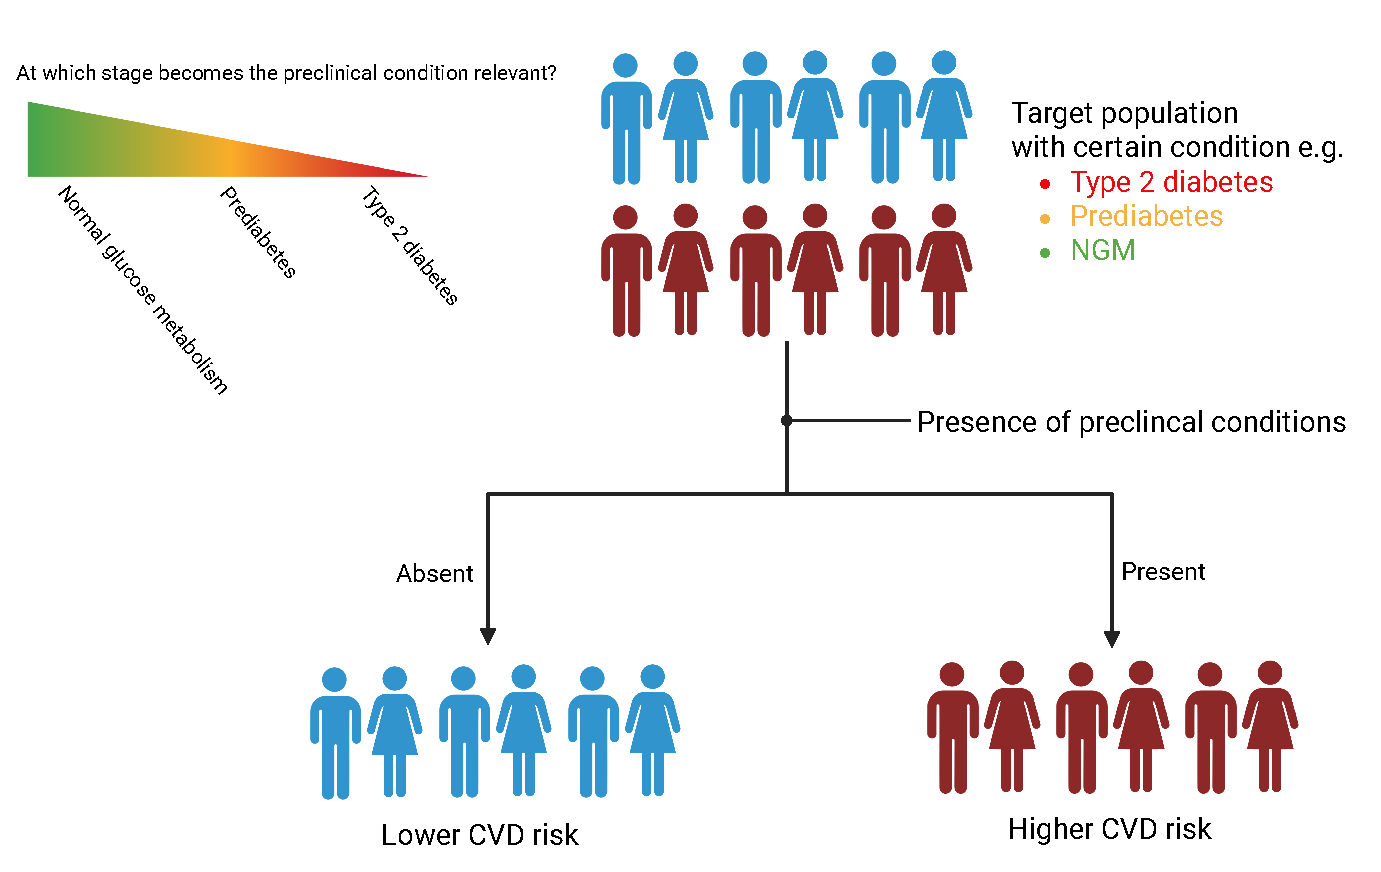
\includegraphics{images/risk_stratification.pdf}

}

\caption{Risk-stratification based on preclinical disease. (Source:
Author)}

}

\end{minipage}%

\end{figure}

Cardiovascular autonomic dysfunction despite it's relationship with
cardiovascular complication has not been used in clinical practice.
Larger epidemiological cohort studies encompassing various stages of
diabetes risk, from normal glucose metabolism to prediabetes, onset of
type 2 diabetes, and longer term progression of type 2 diabetes, serve
as valuable resources for identifying risk-stratification opportunities.
Epidemiological studies provide a broad representation of the target
population, allowing understand the relationship between cardiovascular
autonomic dysfunction and cardiovascular complications. They also have
potential to determine when, along the trajectory of diabetes
progression and duration, autonomic function are meaningful for
cardiovascular risk-stratification.

\bookmarksetup{startatroot}

\hypertarget{aim-and-hypothesis}{%
\chapter{Aim and hypothesis}\label{aim-and-hypothesis}}

The hypotheses of this dissertation are:

CAN and autonomic dysfunction is associated with CVD and acts as an
early risk factor for heart failure and other cardiovascular
complications, including stroke, and myocardial infarction in patients
with prediabetes and/or type 2 diabetes. In addition autonomic
dysfunction is associated with higher levels of sub-clinical meassures
such as carotid-femoral pulse wave velocity and carotid artery
distensibility.

This dissertation investigates the hypothesis by addressing the
following three aims:

Study I: Quantify the cross-sectional association between 24-hour HRV
and subclinical markers of cardiovascular complications: carotid-femoral
pulse wave velocity and carotid artery distensibility, in a participants
with normal glucose metabolism, prediabetes or type 2 diabetes.

Study II: Quantify the longitudinal association of week-long and hourly
HRV with incidence ischemic-CVD, heart failure, and all-cause mortality
in a population with high-risk of diabetes.

Study III: Quantify the cross-sectional association between CAN and
heart failure. Heart failure will be defined by clinical measures
i.e.~N-terminal-pro-BNP (Pro-BNP), WATCH-DM risk, and New York Heart
Association (NYHA) scores among individuals with type 2 diabetes.

\bookmarksetup{startatroot}

\hypertarget{materials-and-methods}{%
\chapter{Materials and methods}\label{materials-and-methods}}

\hypertarget{overview-of-the-studies}{%
\section{Overview of the studies}\label{overview-of-the-studies}}

\begin{longtable}[]{@{}
  >{\raggedright\arraybackslash}p{(\columnwidth - 6\tabcolsep) * \real{0.0588}}
  >{\raggedright\arraybackslash}p{(\columnwidth - 6\tabcolsep) * \real{0.3095}}
  >{\raggedright\arraybackslash}p{(\columnwidth - 6\tabcolsep) * \real{0.3581}}
  >{\raggedright\arraybackslash}p{(\columnwidth - 6\tabcolsep) * \real{0.2685}}@{}}
\caption{Table 1: Overview of studies}\tabularnewline
\toprule\noalign{}
\begin{minipage}[b]{\linewidth}\raggedright
\end{minipage} & \begin{minipage}[b]{\linewidth}\raggedright
Study I
\end{minipage} & \begin{minipage}[b]{\linewidth}\raggedright
Study II
\end{minipage} & \begin{minipage}[b]{\linewidth}\raggedright
Study III
\end{minipage} \\
\midrule\noalign{}
\endfirsthead
\toprule\noalign{}
\begin{minipage}[b]{\linewidth}\raggedright
\end{minipage} & \begin{minipage}[b]{\linewidth}\raggedright
Study I
\end{minipage} & \begin{minipage}[b]{\linewidth}\raggedright
Study II
\end{minipage} & \begin{minipage}[b]{\linewidth}\raggedright
Study III
\end{minipage} \\
\midrule\noalign{}
\endhead
\bottomrule\noalign{}
\endlastfoot
Title & Cardiovascular autonomic dysfunction is linked with arterial
stiffness across glucose metabolism: The Maastricht Study &
Cardiovascular autonomic dysfunction precedes cardiovascular disease and
all-cause mortality: 11-year follow-up in the ADDITION-PRO study &
Cardiovascular autonomic neuropathy and subclinical heart failure in
type 2 diabetes: The CANCAN study \\
Design & Aetiological cross-sectional study & Aetiological prospective
cohort study & Descriptive cross-sectional study \\
Cohort & Maastricht study & ADDITION-PRO study & CANCAN study \\
Study population & 3673 people with normal glucose metabolism,
prediabetes, and type 2 diabetes & 2082 people with high risk of
diabetes & 173 patients with type 2 diabetes visiting outpatients
clinics \\
Data sources & Population-based cohort from The Maastricht Study in the
Netherlands & Cohort study of selected people based on having high risk
of diabetes & Clinical cohort study \\
Determinant & 24-hour HRV & multiday and hourly HRV & Cardiovascular
autonomic reflex test \\
Primary outcome & Arterial stiffness & Major adverse cardiovascular
events, heart failure, and all-cause mortality & NT-proBNP and NYHA
classification? \\
Statistical analysis & Linear regression & Poisson regression & Logistic
regression \\
Missing data & Complete case analysis & Multiple imputation of chained
equations for confounders & Complete case analysis and multiple
imputation of chained equations for CART and confounders \\
\end{longtable}

\hypertarget{study-population}{%
\subsection{Study population}\label{study-population}}

\begin{figure}

{\centering 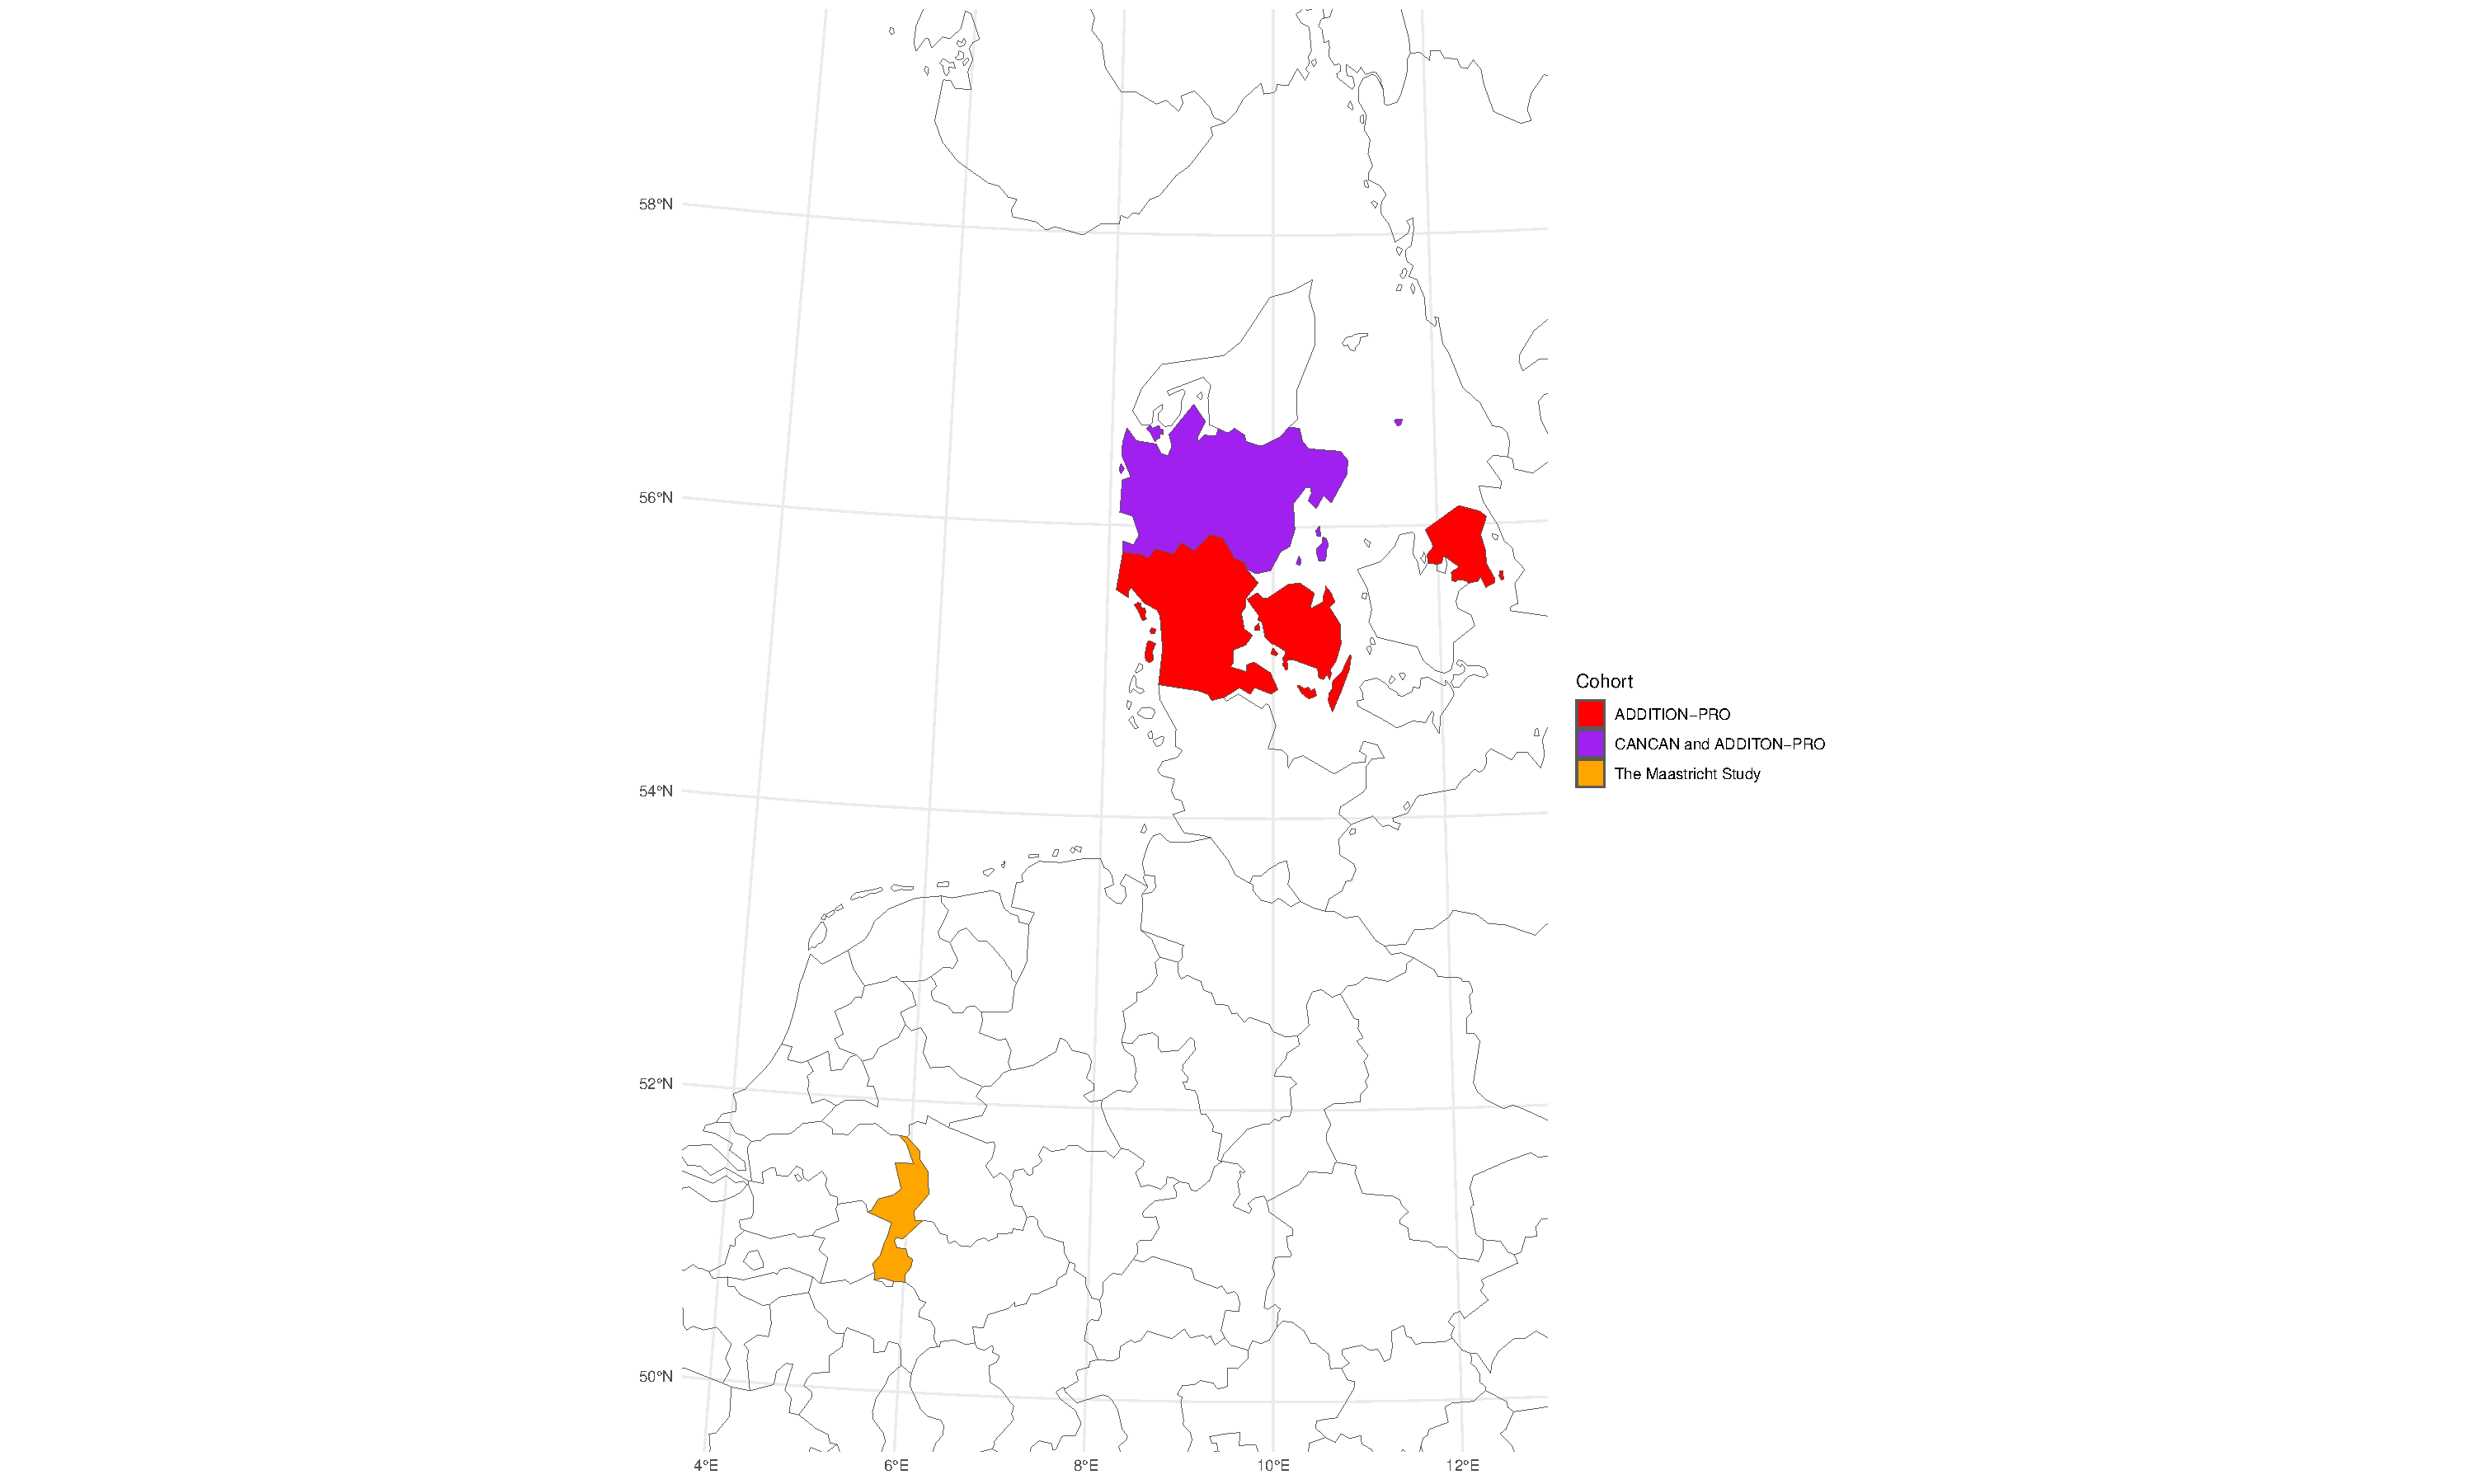
\includegraphics[width=8in,height=\textheight]{images/cohort_map.pdf}

}

\caption{Study populations}

\end{figure}

\hypertarget{study-i---the-maastricht-study}{%
\subsubsection{Study I - The Maastricht
Study}\label{study-i---the-maastricht-study}}

The Maastricht Study is a prospective observational population-based
study of the general population of the province of Limburg, in the
southern part of the Netherlands. The study emphasized the recruitment
of people with type 2 diabetes, through the regional Diabetes Patient
Registry, to extensively phenotype individuals with type 2 diabetes and
those in intermediate stages of the disease. The eligibility criteria
included an age range of 40--70 years. Participants were recruited
through mass media campaigns and mailings from municipal registries
(Gemeentelijke Basis Administratie; GBA). In the analysis of Study I,
the study among 7449 people included participants with measurements of
24-hour HRV and at least one measure of arterial stiffness
(carotid-femoral pulse wave velocity or carotid artery distensibility),
both of which were completed within a three-month period between
November 2010 and December 2020. The study has been approved by the
institutional medical ethics committee (NL31329.068.10) and the Minister
of Health, Welfare and Sports of the Netherlands (Permit
131088-105234-PG). All participants gave written i

\hypertarget{study-ii---addition-pro}{%
\subsubsection{Study II - ADDITION-PRO}\label{study-ii---addition-pro}}

The ADDITION-PRO study is a prospective, population-based cohort nested
within the Danish arm of the ADDITION-Europe study. ADDITION was
originally designed as a stepwise screening program for type 2 diabetes
in general practice, aiming to identify individuals with screen-detected
type 2 diabetes for recruitment into the ADDITION trial. ADDITION-PRO
aims to investigate early markers of CVD and metabolic dysfunction in
individuals in different tiers of diabetes risk.

The ADDITION-Europe screening program identified a large number of
individuals with impaired fasting glucose (IFG), impaired glucose
tolerance (IGT), and normoglycemia despite having risk factors for
diabetes and CVD. Participants for ADDITION-PRO were recruited from the
original ADDITION-DK screening cohort, which included individuals from
190 general practices across Denmark. The recruitment strategy focused
on individuals at high risk of diabetes without type 2 diabetes,
identified through a stepwise screening program that incorporated the
Danish diabetes risk score from the Inter99. This assessment, conducted
between 2001 and 2006, considered factors such as age, sex, history of
gestational diabetes, family history of diabetes, known hypertension,
BMI, and physical activity. High-risk individuals were further screened
for type 2 diabetes using blood measurements, including HbA1c, random
blood glucose, FPG, and OGTT. Those with screen-detected diabetes,
confirmed by a second OGTT, were invited to participate in the ADDITION
trial. High risk individuals without type 2 diabetes were further
considered in as the sampling frame for ADDITION-PRO.

Between 2009 and 2011, a follow-up health examination was conducted at
four ADDITION-DK study centers to establish a cohort baseline. Eligible
participants were those still alive, residing near the research centers
(Steno Diabetes Center Copenhagen, Aarhus University Hospital, Holstebro
Hospital, and the Hospital of South West Jutland, Esbjerg), and who had
not withdrawn consent. Eligibility criteria included individuals aged
40--70 years who had previously undergone diabetes screening in
ADDITION-DK. Exclusion criteria included pregnancy, psychological or
psychiatric disorder preventing informed consent, and life-limiting
conditions. One key feature of the data collection was the precise
measurement of physical activity and energy expenditure using a combined
chest worn accelerometer/heart rate monitor (ActiHeart), which recorded
acceleration and heart rate over a week. In study II, we included
participants with a least 48-hour recording for our first analysis, and
then include those participants with hourly measures of physical
acceleration during the hourly HRV recording for th second analysis. We
also excluded participant with prior CVD ten years before inclusion.

Disease history and follow-up data for the population were obtained from
Denmark's unique national registry system, which allows linkage of
health records using the personal Civil Registration Number assigned to
all citizens. The following national registries were accessed to collect
information on incident CVD and mortality, medication use, and
healthcare utilization: the National Patient Registry (hospital
admissions and outpatient contacts), the National Health Service
Registry (general practice visits), the Medical Prescription Registry,
the Diabetes Registry, and the Cause of Death Registry.

\hypertarget{study-iii---cancan}{%
\subsubsection{Study III - CANCAN}\label{study-iii---cancan}}

The CANCAN Study is an observational study conducted at two hospital
outpatient clinics in Viborg Regional Hospital and Regional Hospital
Gødstrup. It aims to implement a screening protocol for identifying
high-risk individuals using CAN assessments, continuous glucose
monitoring, and heart failure indicators. All measures were part of
routine clinical care for type 2 diabetes in Central Denmark. We
included 200 adults (\textgreater18 years) with type 2 diabetes with
duration of over one year. Exclusion criteria were recent laser-treated
eye disease (≤3 months), pregnancy, lactation, life-threatening illness,
or cognitive impairment preventing consent. Participants were identified
via electronic records and informed about the study by their doctor
during a telephone call. Those interested attended a dedicated meeting
before their annual diabetes exam, where study details were discussed.
Recruitment took place from 2021 to 2024. In study III, participants
without a valid NT-proBNP measurement were excluded.

\hypertarget{study-variables}{%
\section{Study variables}\label{study-variables}}

\hypertarget{measures-for-cardiovascular-autonomic-dysfunction-neuropathy}{%
\subsection{Measures for cardiovascular autonomic dysfunction/
neuropathy}\label{measures-for-cardiovascular-autonomic-dysfunction-neuropathy}}

\begin{figure}

{\centering 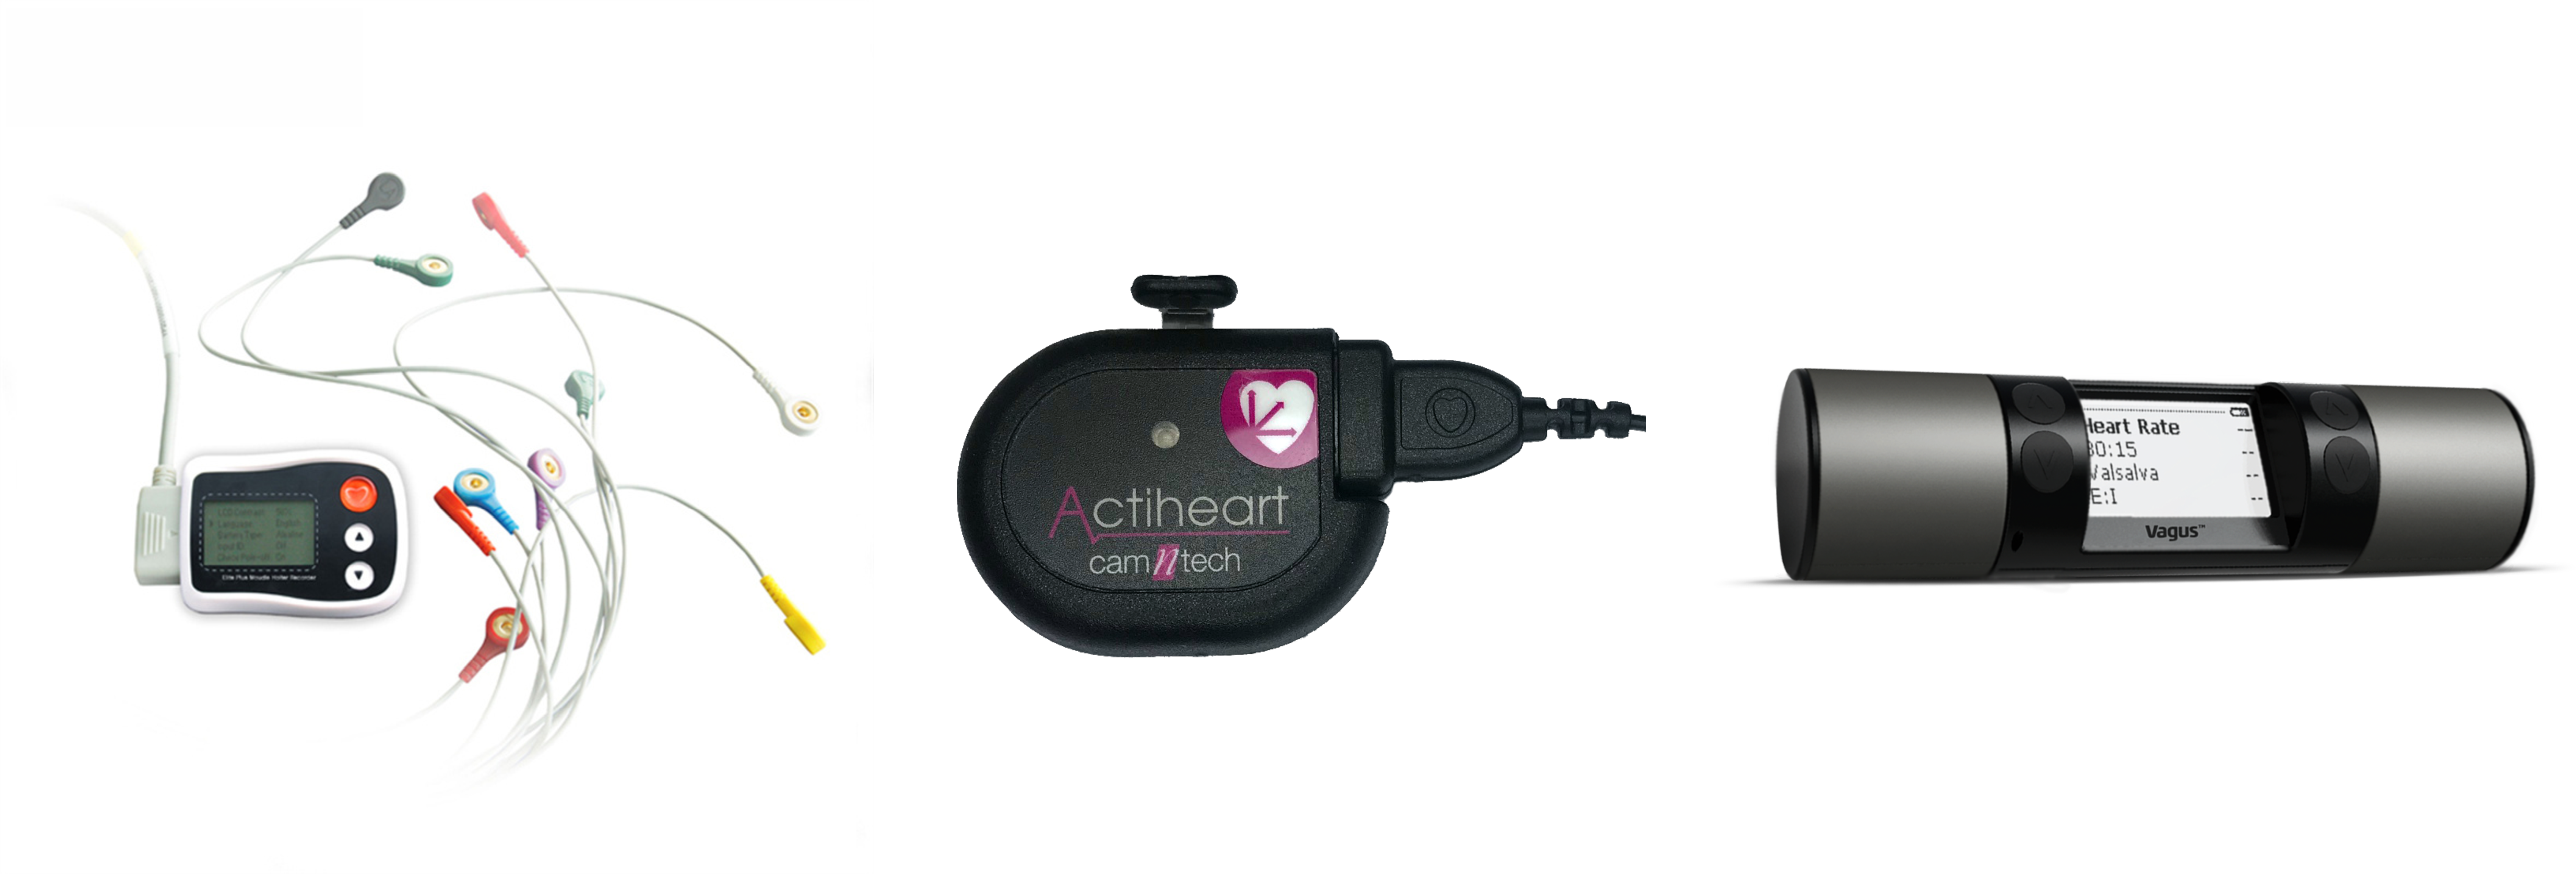
\includegraphics[width=5in,height=\textheight]{images/can_tools.pdf}

}

\caption{Left: Holter monitor Middle: Actiheart Right: Handheld Vagus™
device}

\end{figure}

\textbf{Heart rate variability}

\begin{figure}

\begin{minipage}[t]{\linewidth}

{\centering 

\raisebox{-\height}{

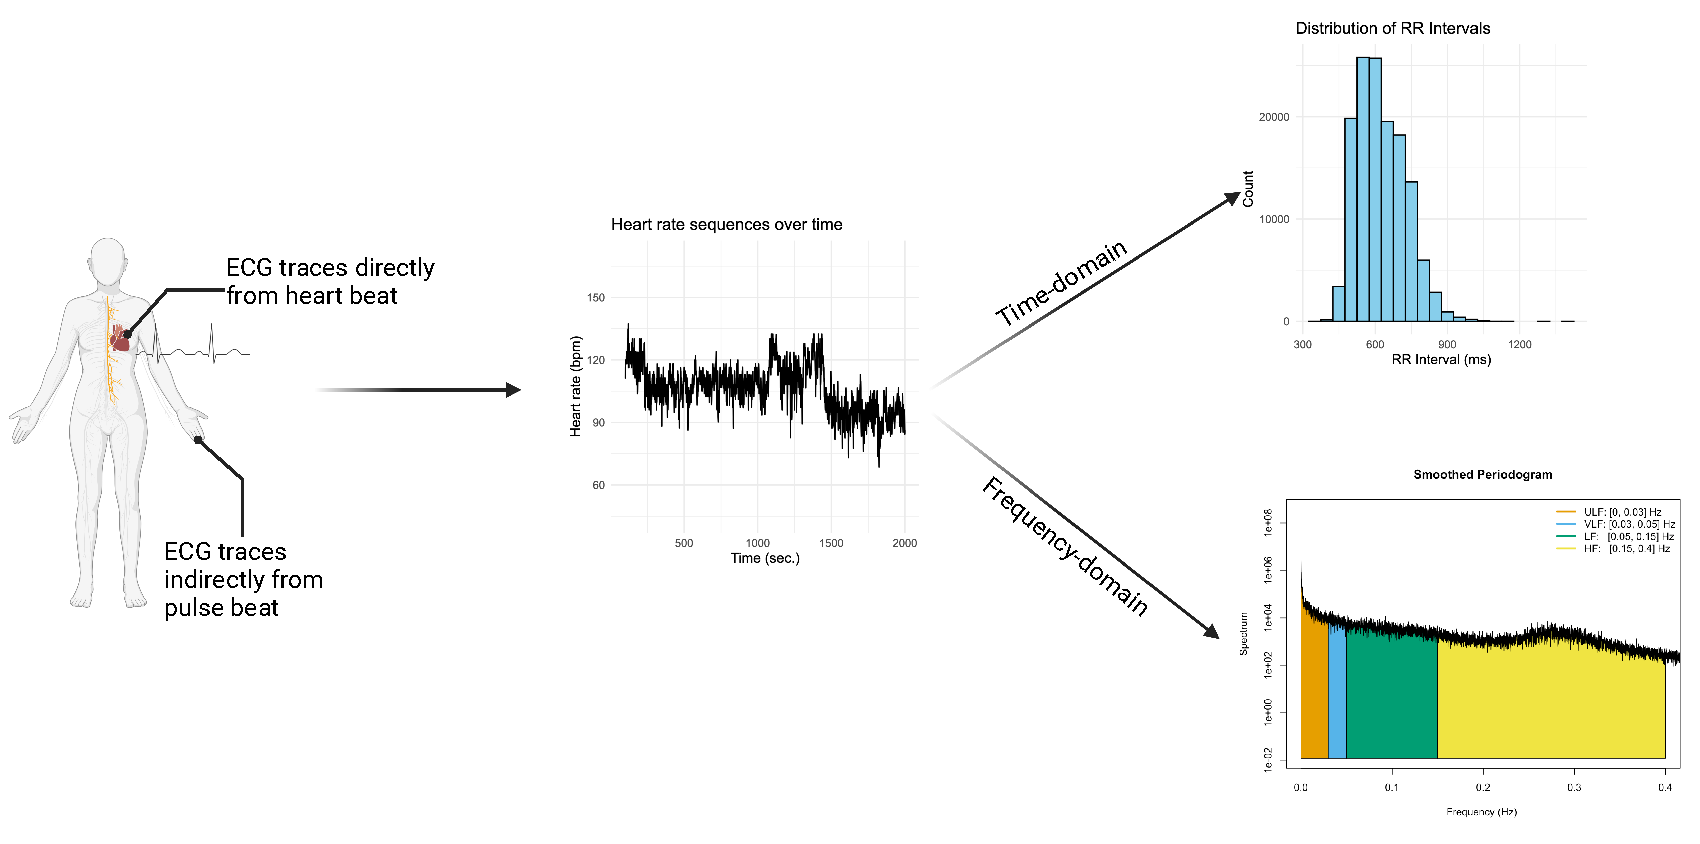
\includegraphics[width=7in,height=\textheight]{images/measurements_hrv.pdf}

}

\caption{Heart rate variability. (Source: Author)}

}

\end{minipage}%

\end{figure}

In study I-III a device was used to capture the distance between each
heartbeat defined as RR intervals from electrocardiogram traces either
directly from heart-beat traces or indirectly from pulse traces. From
this a sequence of successive heart beat intervals is extracted to
calculate HRV. The pool of hearbeat data, we extrapolated time-domain
and frequency-domain HRV indices.

\emph{Time-domain indices}

Time-domain measures of HRV are based on the statistical distribution of
normal-to-normal (NN) heartbeat intervals. Description of time-domain
indices are summarized in \textbf{?@tbl-td}.

\begin{table}

\caption{\textbf{Box 1} Time-domain indices reflections of autonomic
function}\begin{minipage}[t]{\linewidth}

{\centering 

\begin{longtable}[]{@{}
  >{\raggedright\arraybackslash}p{(\columnwidth - 2\tabcolsep) * \real{0.2902}}
  >{\raggedright\arraybackslash}p{(\columnwidth - 2\tabcolsep) * \real{0.7098}}@{}}
\toprule\noalign{}
\begin{minipage}[b]{\linewidth}\raggedright
Time-domain HRV
\end{minipage} & \begin{minipage}[b]{\linewidth}\raggedright
Description
\end{minipage} \\
\midrule\noalign{}
\endhead
\bottomrule\noalign{}
\endlastfoot
\textbf{Standard deviation of NN heart beat intervals (SDNN, in ms)} &
Measures the total variation in interbeat intervals and reflects both
sympathetic and parasympathetic activity\textsuperscript{6}. \\
\textbf{SD of the averages of NN intervals in 5-minute segments
throughout the recording (SDANN, in ms)} & Measures variations in
5-minute mean interbeat intervals, primarily reflecting autonomic
fluctuations associated with the circadian rhythm\textsuperscript{6} \\
\textbf{Mean of the SDs of all NN intervals for all 5-minute segments
(SDNN index, in ms)} & Measures the average short-term variability in
interbeat intervals across successive 5-minute periods, reflecting both
sympathetic and parasympathetic modulation of heart
rate\textsuperscript{6} \\
\textbf{NN50 count divided by the total number of all NN intervals
(pNN50, percentage)} & Measures the proportion of successive interbeat
intervals differing by more than 50 ms, primarily reflecting
parasympathetic (vagal) activity\textsuperscript{50}. \\
\textbf{Square root of the mean of the sum of squares of differences
between adjacent NN intervals (RMSSD, in ms)} & Measures variation in
successive interbeat intervals during inhalation and exhalation,
primarily reflecting parasympathetic (vagal)
activity\textsuperscript{50} \\
\end{longtable}

}

\end{minipage}%

\end{table}

\emph{Frequency-domain indices}

Frequency-domain HRV indices are derived from sequences of NN intervals
transformed into the spectral domain using Fourier transformation. These
indices quantify heart rate oscillations over different timescales.
Short-term variations, such as respiratory sinus arrhythmia, reflect
rapid autonomic changes, while longer oscillations capture autonomic
responses to posture changes, circadian rhythms, or other physiological
processes. Description of frequency-domain indices are summarized in
\textbf{?@tbl-fq}.

\begin{table}

\caption{\textbf{Box 2} Frequency-domain indices reflections of
autonomic function}\begin{minipage}[t]{\linewidth}

{\centering 

\begin{longtable}[]{@{}
  >{\raggedright\arraybackslash}p{(\columnwidth - 2\tabcolsep) * \real{0.2077}}
  >{\raggedright\arraybackslash}p{(\columnwidth - 2\tabcolsep) * \real{0.7923}}@{}}
\toprule\noalign{}
\begin{minipage}[b]{\linewidth}\raggedright
Frequency domain HRV
\end{minipage} & \begin{minipage}[b]{\linewidth}\raggedright
Description
\end{minipage} \\
\midrule\noalign{}
\endhead
\bottomrule\noalign{}
\endlastfoot
\textbf{Variance of all NN intervals ≤ 0.4 Hz, total power (TP, in ms²)}
& Measures the total variation in interbeat intervals, reflecting both
short- and long-term autonomic regulation by the sympathetic and
parasympathetic nervous system\textsuperscript{6}. \\
\textbf{Ultra low-frequency range (ULF, in ms² ≤ 0.003 Hz)} & Measures
very long-term oscillations in interbeat intervals, influenced by
autonomic responses to circadian rhythms, physical activity, metabolic
processes, and thermoregulation
{[}\textsuperscript{51}{]}\textsuperscript{52}. \\
\textbf{Very-low-frequency range (VLF, in ms²; 0.003--0.04 Hz)} &
Measures oscillations in interbeat intervals over 5-minute periods,
reflecting the activity of the renin--angiotensin system and peaks in
sympathetic nervous system activity, while also depending on
parasympathetic
modulation{[}\textsuperscript{53}{]}\textsuperscript{54}. \\
\textbf{Low-frequency range (LF, in ms²; 0.04--0.15 Hz)} & Measures
intermediate oscillations in interbeat intervals, reflecting a
combination of sympathetic and parasympathetic nervous system activity,
particularly associated with baroreflex function and blood pressure
regulation\textsuperscript{55}. \\
\textbf{High-frequency range (HF, in ms²; 0.15--0.4 Hz)} & Measures
short-term oscillations during inspiration and expiration, reflecting
parasympathetic modulation of heart rate via the vagus nerve, and
closely associated with respiratory sinus
arrhythmia\textsuperscript{56}. \\
\end{longtable}

}

\end{minipage}%

\end{table}

\textbf{Holter recordings in study I}

All ECG recordings were obtained using a 12-lead Holter system
(Fysiologic ECG Services, Amsterdam, the Netherlands) over 24 hours, as
previously described. Participants were instructed to follow their
regular daily activities but avoid showering during the recording. The
ECG data were processed using proprietary Holter Analysis Software
(Fysiologic ECG Services), where artefacts and ectopic beats were
excluded through automated processing and manual validation. A minimum
recording duration of 18 hours was required for further analysis.
Inter-beat intervals between consecutive sinus beats were provided in
milliseconds (ms). Time-domain HRV indices were calculated, including
SDNN, SDANN, RMSSD, SDNN index, and pNN50. Frequency-domain measures
were derived using Fast Fourier Transform, including TP, ULF, VLF, LF,
and HF. Outliers were removed. HRV indices were standardised by their
mean and SD, and composite Z-scores were computed for time and
frequency-domain measures, respectively. This selection of indices
covers the main sources of HRV variance.

\textbf{ActiHeart heart rate and physical activity in study II}

Heart rate was measured using a combined accelerometer and heart rate
monitor (ActiHeart, CamNTech, Cambridge, UK), recording uniaxial
acceleration and heart rate. The data collection and processing methods
have been described previously. Mean heart rates were recorded in
30-second epochs, and HRV was derived as the variation between
consecutive normal heartbeats on the ECG. HRV calculations were
performed using the RHRV package (version 4.2.7) in R, including SDNN,
SDANN, SDNN index, TINN, and mean HR (mHR). We tested our approach on a
dataset with full access to all interbeat intervals to validate our
algorithm\textsuperscript{57}. These indices have shown high validity
for HRV indices based on global distribution (e.g.~SDNN, SDANN, SDNNi)
in 24-hour recordings. HRV indices were calculated by week, 24-hour
cycle, and hour of the day, with hourly values averaged across recording
days.

\textbf{Vagus device for cardiovascular autonomic reflex test in study
III}

CAN was diagnosed using cardiovascular autonomic reflex tests (CARTs),
the gold standard for CAN assessment. R-R intervals were derived from an
ECG signal using the Vagus™ device (Medicus Engineering, Aarhus,
Denmark). We used pulse rate ratios measured under different conditions.
Three standardized cardiovascular autonomic reflex tests (CARTs) were
performed---lying-to-standing, deep breathing, and the Valsalva
manoeuvre, following a standardized protocol conducted between 8:00 a.m.
and 2:00 p.m., after 10 minutes of supine rest. Smoking and caffeine
intake were prohibited two hours before testing. Each test was conducted
once by trained examiners.

Manifest CAN was defined as two or more abnormal CARTs using
age-specific cut-off values (ref.). The Vagus™ device's accuracy has
been validated against FDA standards and stationary devices, showing
moderate to high reproducibility (ref.).

\begin{figure}

\begin{minipage}[t]{\linewidth}

{\centering 

\raisebox{-\height}{

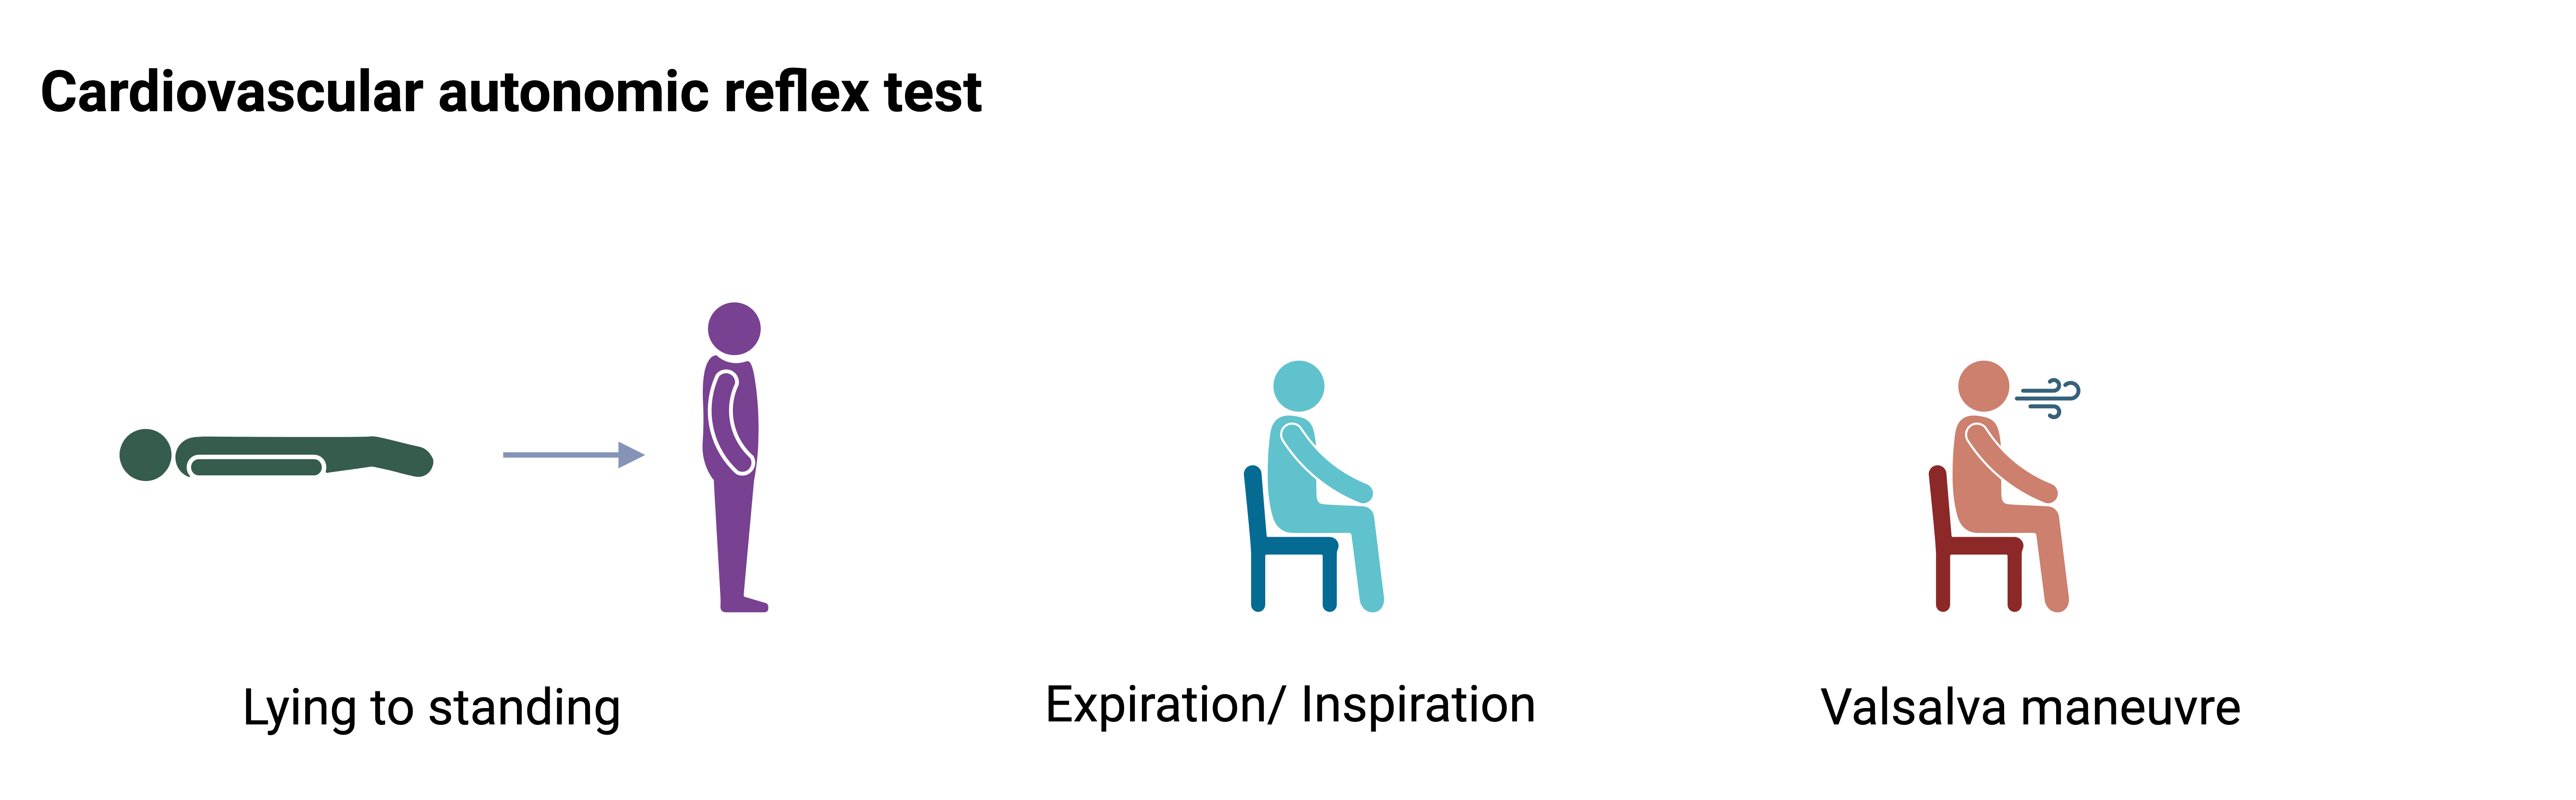
\includegraphics{images/cart.png}

}

\caption{CART}

}

\end{minipage}%

\end{figure}

HRV was derived from all CARTs using autoregressive spectral analysis.
Time domain measures included SDNN and RMSSD, while frequency domain
measures included LF, HF, and total power. Orthostatic hypertension was
defined as a sustained drop in systolic blood pressure of ≥20 mmHg or
diastolic blood pressure of ≥10 mmHg within three minutes of standing
(ref.).

\hypertarget{confounders-and-variables-for-instrumental-bias}{%
\subsection{Confounders and variables for instrumental
bias}\label{confounders-and-variables-for-instrumental-bias}}

Across Studies I, II, and III, a comprehensive set of covariates and
potential confounders were assessed, including lifestyle factors,
clinical measurements, biochemical markers, and socioeconomic
indicators.

Smoking status was self-reported in all studies, categorized as never,
former, or current (Study I), current/ex/never (Study II), and
smoker/non-smoker (Study III). Alcohol consumption was recorded as
average weekly units in all three studies. Physical activity was
assessed via self-report in Studies I, II, III, with Study I capturing
total and moderate-to-vigorous activity (hours/week), Study II used the
Recent Physical Activity Questionnaire (RPAQ) to calculate physical
activity energy expenditure (PAEE), and Study III classifying activity
as sedentary or non-sedentary. In Study II also used combined
accelerometry and heart rate monitoring (ActiHeart) to estimate PAEE.
Study II included register-based data on socioeconomic status at
baseline, including education length, income, and employment status. All
studies included measurements of body mass index (BMI), waist
circumference, and systolic and diastolic blood pressure, obtained
during clinical examinations.

Blood samples were analyzed in all studies for HbA1c, fasting plasma
glucose (FPG), triglycerides, total cholesterol, high-density
lipoprotein (HDL), and low-density lipoprotein (LDL) cholesterol. Study
I also included a 2-hour oral glucose tolerance test (OGTT) to classify
glucose metabolism status based on FPG and OGTT (normal, prediabetes,
type 2 diabetes) using WHO 2006 criteria, excluding HbA1c as a
diagnostic criterion. Study III additionally measured creatinine,
estimated glomerular filtration rate (eGFR), and urine
albumin-to-creatinine ratio.

Self-reported history of cardiovascular disease (CVD) and use of
anti-hypertensive, glucose-lowering, and lipid-lowering medications were
collected in all studies. In Study II, history of CVD events in the 10
years prior to baseline were retrieved from national registers. In Study
III, history of CVD was collected electronic patient records.

\hypertarget{outcomes}{%
\section{Outcomes}\label{outcomes}}

\hypertarget{arterial-stiffness}{%
\subsection{Arterial stiffness}\label{arterial-stiffness}}

Arterial stiffness characterized arteriosclerosis and atherosclerosis
properties of the arteries. The stiffness of different trees of the
vascular musculature can assessed both locally and dynamically. Aortic
and carotid stiffness were assessed as markers of arterial stiffness,
following previously described procedures\textsuperscript{58}.

\textbf{Pulse wave velocity}

Aortic stiffness was measured by carotid-femoral pulse wave velocity
(cf-PWV) using applanation tonometry (SphygmoCor, Atcor Medical, Sydney,
Australia), with the median of at least three consecutive recordings
included in the analysis. cf-PWV is calculated from the time between the
ECG systole and the arrival of the pressure wave at the femoral and
carotid measurement sites and the distance between these two measurement
sites. It is measured with participants in a supine position following a
10-minute rest period. The aortic path length was determined using a
tape measure by subtracting the carotid-to-sternal notch distance from
the femoral-to-sternal notch distance\textsuperscript{58}.

\textbf{Carotid artery distensibility}

Carotid stiffness was assessed by the carotid artery distensibility
coefficient (CD), based on ultrasound imaging of the left common carotid
artery using a 7.5 MHz linear probe (MyLab 70, Esaote Europe,
Maastricht, the Netherlands). CD was calculated as ΔD/braPP, where ΔD
represents carotid distension and braPP is brachial pulse pressure. Mean
heart rate and mean arterial pressure (MAP) were recorded every five
minutes using an oscillometer device (Accutorr Plus, Datascope,
Montvale, NJ, USA)\textsuperscript{58}..

\begin{figure}

\begin{minipage}[t]{\linewidth}

{\centering 

\raisebox{-\height}{

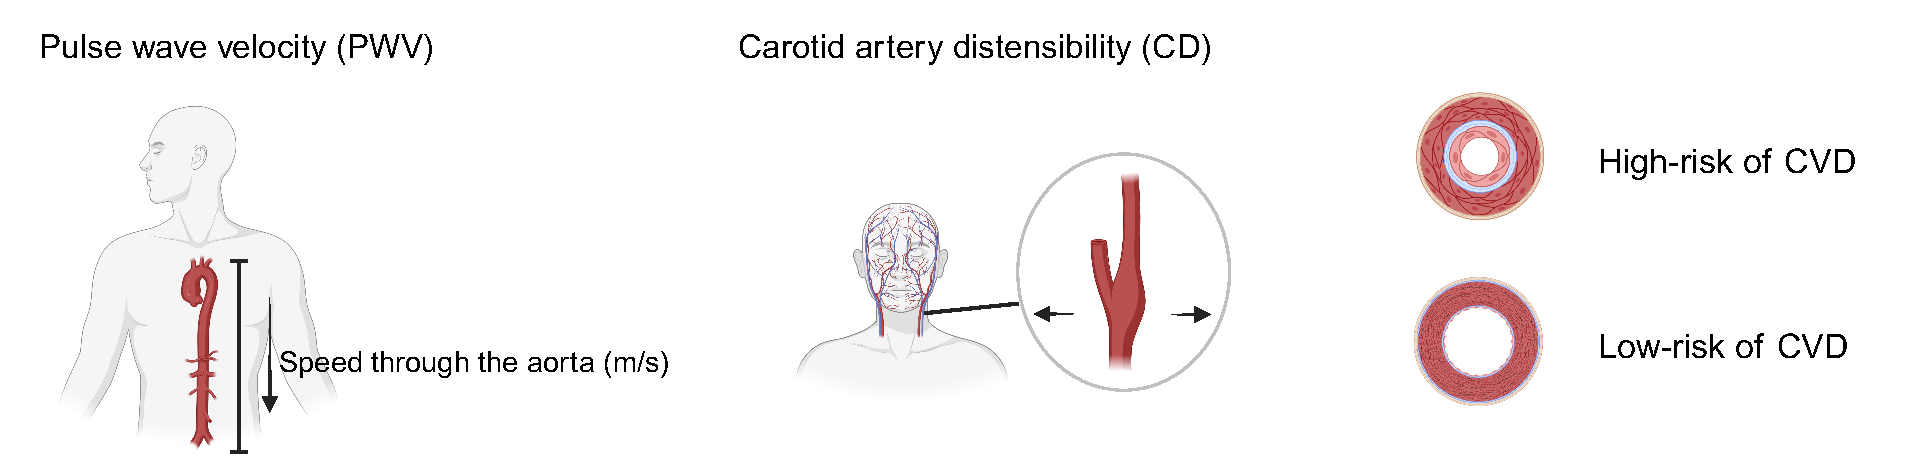
\includegraphics{images/Methods_arterial_stiffness.pdf}

}

\caption{Measures of arterial stiffness, measured dynamically at the
aortic and local carotid sites. (Source: Author)}

}

\end{minipage}%

\end{figure}

\hypertarget{indicators-of-heart-failure}{%
\subsection{Indicators of heart
failure}\label{indicators-of-heart-failure}}

N-terminal prohormone of brain natriuretic peptide (NT-proBNP) is a
neuretic peptide that can be used to detect patients with heart failure
and the progression. It derives from B-type natriuretic peptid (BNP)
which is a cardial neurohormon, that is syntezied and secreted as
response to streched cariomycytes and cardiac volume overload. After
secretion, proBNP is cleaved, releasing the active hormone BNP along
with the remaining N-terminal fragment, known as NT-proBNP. In Study
III, blood sample were taken at Study cite. Description of the NT-proBNP
analysis of plasma samples is described in supplementary material
{[}ref.{]}.

We used a modified version validated The WATCH-DM heart failure risk
score. The risk score is based on 9 variables: two binary (history of
myocardial infarction and coronary artery bypass grafting) and seven
continuous (age, BMI, systolic/diastolic BP, serum creatinine, HDL
cholesterol, and HbA1c). Scores range from 0--39, categorized as very
low (≤11), low (12--13), moderate (14--15), high (16--18), and very high
(≥19) risk.

NYHA class stage I-IV was included. Heart failure symptoms were defined
as NYHA class II--IV, assessed by a physician.

\hypertarget{cardiovascular-events}{%
\subsection{Cardiovascular events}\label{cardiovascular-events}}

Information on CVD events and mortality was obtained from the Danish
National Patient Registers until 2021. ICD-10 codes for stroke,
myocardial infarction, cardiovascular death, cardiovascular
revascularization, and heart failure. We defined three-point major
adverse cardiovascular events (MACE) as myocardial infarction, stroke,
cardiovascular revascularization, and cardiovascular death.

\begin{table}

\caption{\textbf{?(caption)}}\begin{minipage}[t]{\linewidth}

{\centering 

\begin{longtable}[]{@{}
  >{\raggedright\arraybackslash}p{(\columnwidth - 2\tabcolsep) * \real{0.2267}}
  >{\raggedright\arraybackslash}p{(\columnwidth - 2\tabcolsep) * \real{0.7733}}@{}}
\toprule\noalign{}
\endhead
\bottomrule\noalign{}
\endlastfoot
\textbf{Outcome} & \textbf{Diagnosis codes} \\
\emph{Heart failure} & ICD: I50 \\
\emph{Three-point MACE} & \\
\begin{minipage}[t]{\linewidth}\raggedright
\begin{itemize}
\tightlist
\item
  Stroke
\end{itemize}
\end{minipage} & ICD: I61 - I64 \\
\begin{minipage}[t]{\linewidth}\raggedright
\begin{itemize}
\tightlist
\item
  Myocardial infarction
\end{itemize}
\end{minipage} & ICD: I21-I24 \\
\begin{minipage}[t]{\linewidth}\raggedright
\begin{itemize}
\tightlist
\item
  Cardiovascular death
\end{itemize}
\end{minipage} & ICD: I20-I28, I42, I46 \\
\begin{minipage}[t]{\linewidth}\raggedright
\begin{itemize}
\tightlist
\item
  Cardiovascular revascularization
\end{itemize}
\end{minipage} & SKA: KPAE10, KPAE25, KPAF10, KPAF20, KPAF21, KPAF22,
KPAH10, KPAH20, KPAH21, KPEE, KPEF, KPEH, KPEP, KPEQ, KPFE,, KPFH, KPFP,
KPFQ \\
\end{longtable}

}

\end{minipage}%

\end{table}

\hypertarget{statistical-methods}{%
\section{Statistical Methods}\label{statistical-methods}}

\hypertarget{cross-sectional-analysis}{%
\subsection{Cross-sectional analysis}\label{cross-sectional-analysis}}

In Study I, we used multiple linear regression to investigate
associations between multiday HRV and arterial stiffness. Model 1
adjusted for age, sex, education, glucose metabolism status, and mean
arterial pressure (MAP) to account for the oversampling of individuals
with type 2 diabetes and potential instrumental bias of arterial
pressure flow. Model 2 included additional adjustments for smoking
behavior, alcohol consumption, physical activity, body mass index,
HbA1c, triglycerides, total-to-HDL cholesterol ratio, and medication
use. Arterial stiffness measures were log-transformed to ensure normally
distributed residuals and back-transformed into percentage change
estimates. We add interaction sex to oberve if the association differed
between sex. We performed sensitivity analyses excluding individuals on
antihypertensive treatment or glucose-lowering medication. In Study III,
we applied logistic regression models to investigate the association
between CAN and heart failure, using NT-proBNP as the primary outcome.
We adjusted for age, sex, and diabetes duration, smoking behavior,
alcohol consumption, body mass index, HbA1c, triglycerides, total
cholesterol, and antihypertensive medication, eGFR and prior CVD. We
performed sensitivity analyses excluded participants with beta-blocker
treatment or prior CVD.

\hypertarget{time-to-event-analysis}{%
\subsection{Time-to-event analysis}\label{time-to-event-analysis}}

In Study II, we used Poisson regression models to quantify the
associations between HRV and cardiovascular events, as follow-up data
were undisturbed over time and to avoid assumptions of proportional
hazards\textsuperscript{59}. Multiday HRV was modelled using splines
with knots at predefined percentiles to assess non-linear associations.
Hourly HRV was analysed separately for each hour to observe if the
association of HRV had diurnal variation. Both HRV and mHR were
standardized by their mean and standard deviation to ensure
comparability. Based on assumptions about potential confounding pathways
summarized in directed acyclic graphs (DAG), we fitted two models: Model
1 adjusted for age and sex, while Model 2 further adjusted for
education, smoking, alcohol consumption, physical activity (physical
activity energy expenditure (PAEE) calculated from Recent Physical
Activity Questionnaire RPAQ), body mass index, total cholesterol, and
HbA1c. Additional analyses were performed with HRV pre-adjusted for
concurrent heart rate and physical acceleration to account the influence
of these factors. Missing covariates were handled using multiple
imputation. {[}Add age specific incidence rates{]}

\hypertarget{effect-modification-det-kan-evt.-kortes-ned}{%
\subsection{Effect modification {[}det kan evt. kortes
ned{]}}\label{effect-modification-det-kan-evt.-kortes-ned}}

Effect modification is used to assess whether the association between an
exposure and an outcome varies depending on the level of a third
variable, known as the effect modifier. This means that the observed
relationship between the exposure and the outcome is not uniform across
all subgroups. Instead, it differs across strata defined by the effect
modifier\textsuperscript{60}.

In Study I, we hypothesize that the association between 24-hour and
arterial stiffness was stronger in strata of progression of diabetes
(normal glucose metabolism, prediabetes, type 2 diabetes). We therefore
first stratified by diabetes status to observe the size of the
association across strata. We then combine all groups and include an
interaction term between HRV and diabetes status. We did subsidiary
analysis to check if the effect was modified by dysglycemia by
stratifying HbA1c and fasting plasma glucose into deciles. In Study II,
we quatified whether the association between multiday HRV and CVD
endpoints varied by sex to explore potential biological dimorphism.

In Study III, we aimed to determine whether the association between CAN
and elevated NT-proBNP is present in the subgroup without symptoms,
defined as NYHA class \textless{} II. Hence, we hypothesized no
significant effect modification between groups with and without
symptoms. Similarly, we explored whether the association remains present
in the group classified as low to moderate risk of heart failure, based
on the WATCH-DM risk score.

A significant effect modification between the exposure and the effect
modifier in all analyses was defined as an interaction term with a
p-value \textless{} 0.05.

\hypertarget{multiple-imputed-by-chained-equations}{%
\subsection{Multiple imputed by chained
equations}\label{multiple-imputed-by-chained-equations}}

Multiple Imputation by Chained Equations (MICE) is a method for handling
missing data in datasets. This procedure imputes missing values through
an iterative series of predictive models, generating plausible estimates
while preserving the relationships within the data. To avoid one
imputation for missing value could give the value the same confidence as
the a non-missing value, we followed Rubins Rule. Rubin's rules in MICE
combine results from multiple imputed datasets by pooling estimates of
interest (e.g., means or regression coefficients) using their within-
and between-imputation variances. Thus, we ensure valid statistical
inferences by accounting for the uncertainty introduced by missing data.

In Study II, we imputed confounders to include as many participants and
avoid excluding population with our without cardiovascular or mortality
events. We imputed dataset 10 times. In Study III, we imputed missing
CART, as a proportion of participants had non-valid test due to
insufficient air in the valsalva manuevre, unstable heart beats or data
error. These variables was used as auxiliary variables in imputation to
reduce bias\textsuperscript{61}. All available variables of biochemical
measures, diagnosis, medication and cause of non-valid CART was used to
impute each missing CART using predictive mean matching.

\hypertarget{instrumental-bias}{%
\subsection{Instrumental bias}\label{instrumental-bias}}

In Study I-III we are investigating the body properties by dynamic
measures and biomarkers to quantify autonomic function, arterial
stiffness, and cardiac function. Other conditions may affect the
properties we are attempting to measure, and thus are causing
instrumental bias.

\emph{Vascular Stiffness}

In Study I, we used measurements of arterial stiffness using cf-PWV and
carotid distensibilty. Both measures are influenced by arterial pressure
at the time of examination. Arterial pressure affects the propagation of
the pressure wave through the aorta (cf-PWV) and the expansion and
contraction of the carotid artery (carotid distensibilty) {[}ref.{]}. To
account for this, we adjusted for mean arterial pressure in our models.

\emph{Cardiovascular autonomic function}

In Study II, we assessed cardiovascular autonomic function using
multiday HRV recordings and hourly HRV measurements. Studies have
highlighted that HRV is dependent on heart rate, and low HRV may simply
reflect a higher resting heart rate (rHR). To adjust for this without
overcorrecting for a collinear variable, we pre-adjusted HRV by
regressing rHR on HRV, extracting the residuals, and using these as the
pre-adjusted determinant. For hourly HRV, variability in heart rate may
be influenced by changes in physical activity, creating a risk that HRV
serves as a proxy for movement rather than autonomic function. To
address this, we applied a similar pre-adjustment approach by regressing
concurrent heart rate and physical acceleration to account for physical
activity.

\emph{Biomarker of Heart Failure}

In Study III, kidney function and overweight are know to influence
NT-proBNP levels independently of heart failure. We adjusted the model
to account for the blurred effect of eGFR on NT-proBNP levels in the
analysis.

\bookmarksetup{startatroot}

\hypertarget{results}{%
\chapter{Results}\label{results}}

In this section, I will summarize study population characteristics and
findings from analysis.

\hypertarget{study-i}{%
\section{Study I}\label{study-i}}

\hypertarget{descriptive}{%
\subsection{Descriptive}\label{descriptive}}

In The Maastricht Study, {[}10,000 participated by Date{]}, of those
1316 reported prior CVD. Participants who had valid 24-hour HRV measured
was 4379 and of those 3673 had a valid measurement of either CD or
cf-PWV. Study population included 3673 participants. Further
characteristic are described in the study I manuscript {[}Table 1{]}
{[}refeernce to study I{]}.

\hypertarget{tbl-ms}{}
\begin{table}
\caption{\label{tbl-ms}Study charteristics by diabetes status }\tabularnewline

\centering
\resizebox{\linewidth}{!}{
\begin{tabular}{l|l|l|l}
\hline
**Characteristic** & **Normal glucose metabolism**  
N = 2,389 & **Prediabetes**  
N = 538 & **Type 2 Diabetes**  
N = 746\\
\hline
Sex &  &  & \\
\hline
Men & 1,028 (43\%) & 280 (52\%) & 481 (64\%)\\
\hline
Women & 1,361 (57\%) & 258 (48\%) & 265 (36\%)\\
\hline
Age (years) & 58 (51, 64) & 62 (57, 68) & 63 (57, 68)\\
\hline
Total physical activity (hours/week) & 13 (9, 19) & 13 (9, 19) & 12 (7, 17)\\
\hline
Moderate to vigorous physical activity (hours/week) & 5.3 (3.0, 8.3) & 4.5 (2.3, 7.5) & 3.8 (1.5, 6.8)\\
\hline
BMI (kg/m²) & 25.0 (22.9, 27.4) & 27.2 (24.9, 30.1) & 28.8 (26.0, 31.7)\\
\hline
Waist (cm) & 89 (81, 97) & 98 (90, 105) & 103 (96, 112)\\
\hline
HbA1c (\%) & 5.35 (5.17, 5.63) & 5.63 (5.35, 5.90) & 6.54 (6.08, 7.09)\\
\hline
Fasting plasma glucose (mmol/L) & 5.10 (4.80, 5.40) & 5.90 (5.40, 6.30) & 7.40 (6.60, 8.50)\\
\hline
LDL (mmol/L) & 3.20 (2.70, 3.90) & 3.30 (2.60, 4.00) & 2.40 (1.80, 3.10)\\
\hline
HDL (mmol/L) & 1.60 (1.30, 2.00) & 1.40 (1.20, 1.80) & 1.30 (1.00, 1.50)\\
\hline
Total cholesterol (mmol/L) & 5.50 (4.80, 6.20) & 5.50 (4.80, 6.30) & 4.50 (3.90, 5.20)\\
\hline
Triglycerides (mmol/L) & 1.05 (0.80, 1.45) & 1.39 (1.03, 1.90) & 1.51 (1.08, 2.14)\\
\hline
Duration of type-2 diabetes (only for diagnosed participants) & NA (NA, NA) & NA (NA, NA) & 3 (0, 9)\\
\hline
Mean IBI (ms) & 838 (775, 907) & 815 (760, 897) & 806 (744, 889)\\
\hline
SDNN (ms) & 138 (117, 164) & 127 (106, 152) & 116 (96, 139)\\
\hline
RMSSD (ms) & 26 (21, 34) & 24 (19, 33) & 22 (17, 31)\\
\hline
SDANN (ms) & 125 (103, 149) & 113 (92, 139) & 103 (84, 127)\\
\hline
SDNNi (ms) & 55 (46, 65) & 50 (41, 60) & 44 (36, 54)\\
\hline
pNN50 (\%) & 7 (3, 13) & 5 (2, 10) & 4 (2, 9)\\
\hline
TP (ms²) & 12,596 (8,880, 17,498) & 10,615 (7,134, 15,374) & 8,880 (6,064, 12,722)\\
\hline
ULF (ms²) & 10,771 (7,392, 15,142) & 8,948 (5,852, 13,374) & 7,524 (5,036, 11,001)\\
\hline
VLF (ms²) & 1,198 (833, 1,692) & 1,015 (685, 1,478) & 816 (541, 1,267)\\
\hline
LF (ms²) & 421 (257, 651) & 328 (200, 540) & 261 (154, 422)\\
\hline
HF (ms²) & 94 (57, 158) & 78 (47, 138) & 63 (36, 117)\\
\hline
Systolic blood pressure (mmHg) & 123 (114, 133) & 129 (122, 140) & 130 (122, 139)\\
\hline
Diastolic blood pressure (mmHg) & 75 (71, 80) & 78 (73, 83) & 76 (72, 81)\\
\hline
Mean arterial pressure (mmHg) & 95 (88, 102) & 99 (93, 107) & 98 (92, 105)\\
\hline
Carotid artery distensibility (10-3/kPa) & 15.0 (11.8, 18.8) & 13.5 (10.4, 16.9) & 12.5 (9.9, 16.0)\\
\hline
Carotid-femoral pulse wave velocity (m/s) & 8.08 (7.28, 9.16) & 8.96 (7.84, 10.32) & 9.36 (8.16, 10.80)\\
\hline
N\_HT & 833 (35\%) & 317 (59\%) & 590 (79\%)\\
\hline
Antihypertensive medication & 431 (18\%) & 199 (37\%) & 478 (64\%)\\
\hline
med\_HT\_beta & 149 (6.2\%) & 77 (14\%) & 195 (26\%)\\
\hline
Lipid-lowering medication & 280 (12\%) & 141 (26\%) & 484 (65\%)\\
\hline
\end{tabular}}
\end{table}

\hypertarget{hour-hrv-and-arterial-stiffness}{%
\subsection{24-hour HRV and arterial
stiffness}\label{hour-hrv-and-arterial-stiffness}}

\textbf{Time-domain HRV}

In the fully adjusted model 2, cf-PWV was 2.8\% (CI: 2.1; 3.4) lower,
while CD was 3.3\% (CI: 1.5; 5.1) higher per SD higher in HRV
time-domain Z-score. Among the time-domain indices, SDNN, SDNNi, and
SDANN showed the strongest associations, with cf-PWV being lower by
2.5\% (CI: 2.0; 3.1), 2.5\% (CI: 1.9; 3.4), and 2.2\% (CI: 1.7; 2.7),
respectively. Conversely, CD was higher by 3.2\% (CI: 1.7; 4.7), 3.0 \%
(CI: 1.4; 4.6), and 2.8\% (CI: 1.3; 4.3), respectively. RMSSD and pNN50
showed a weaker association with cf-PWV (-1.1\% {[}CI: -1.4; -0.4{]},
and -1.1 {[}-1.7; -0.6{]}), while no evidence for an association was
found with CD.

\textbf{Frequency-domain HRV}

In the fully adjusted model 2, cf-PWV was 2.8\% (CI: 2.1; 3.5) lower,
while CD was 3.2\% (CI: 1.3; 5.1) higher per SD higher in HRV
frequency-domain Z-score. Among the frequency-domain indices, total
power, VLF, and ULF showed the strongest associations, with cf-PWV being
lower by 2.2\% (CI: 1.7; 2.8 ), 2.4\% (CI: 1.9; 4.0), and 2.1\% (CI:
1.5; 2.6), respectively. Conversely, CD was higher by 2.7\% (CI: 1.2;
4.2), 2.4\% (CI: 0.9; 4.1), and 2.6\% (CI: 1.1; 4.1), respectively. HF
showed a weaker association with cf-PWV (-0.9\% {[}CI: -1.4; -0.4{]}),
while no evidence for an association was found with CD. Mean interbeat
interval was associated with 2.4 \% (CI: 1.8; 2.9) lower cf-PWV and
4.5\% (3.1; 6.1) higher CD.

\hypertarget{effect-modification-of-diabetes-status}{%
\subsection{Effect modification of diabetes
status}\label{effect-modification-of-diabetes-status}}

The study population represented diabetes risk of normal glucose
metabolism (65\%), prediabetes (15\%), and type 2 diabetes (20\%). The
median (IQR) cf-PWV (aortic stiffness) became higher with diabetes
status: NGM: 8.08 m/s (7.28, 9.16), prediabetes: 8.96 m/s (7.84, 10.32),
and type 2 diabetes: 9.36 m/s (8.16, 10.80). CD (carotid stiffness)
decreased: NGM: 15.0 (11.8, 18.8), prediabetes: 13.5 (10.4, 16.9), and
type 2 diabetes: 12.5 (9.9, 16.0) × 10⁻³/kPa. SDNN (ms) was highest in
NGM and decreased with worsening glucose metabolism: NGM: 138ms (117,
164), prediabetes: 127ms (106, 152), and type 2 diabetes: 116ms (96,
139). Further description of charaterisitcs by diabetes are described in
Table~\ref{tbl-ms}.

The association between HRV time-domain Z-scores and cf-PWV and CD was
significantly modified by prediabetes (cf-PWV: -4.9 {[}CI: -6.523;
-3.243{]} \(^{interaction(*) ^{p-value< 0.01}}\) CD: 8.0 {[}CI:3.8;
12.5{]}\(^{*^{p-value< 0.01}}\)) but not by type 2 diabetes (cf-PWV:
-3.5 \% {[}CI: -4.8; -2.1){]} \(^{*^{p-value< 0.1}}\) CD: 4.8 \%
{[}CI:1.3; 8.4{]}\(^{*^{p-value< 0.1}}\)). For the indices SDNN and
SDANN, the association with both cf-PWV and CD was significantly
modified by both prediabetes and type 2 diabetes.

The association between HRV frequency-domain Z-score and cf-PWV was
significantly modified from normal glucose metabolism by prediabetes
(-5.7 \%{[}CI:-7.4; -3.9{]}\(^{*^{p-value< 0.01}}\)) and type 2 diabetes
(-3.9 \%{[}CI:-5.4; -2.3{]}\(^{*^{p-value< 0.05}}\)) while CD was only
modified by prediabetes (8.3 \%{[}CI:3.6;
13.2{]}\(^{*^{p-value< 0.01}}\)) but not by type 2 diabetes (5.3
\%{[}CI:1.4; 9.4{]}\(^{*^{p-value< 0.1}}\)). For the indices total power
and ULF, the association with both cf-PWV and CD was significantly
modified by both prediabetes and type 2 diabetes. Mean inter beat
interval association with cf-PWV or CD was not significantly modified by
diabetes status.

As I did not observe a stepwise increase in the modification of glucose
metabolism status from prediabetes to type 2 diabetes, I excluded the
subgroup with type 2 diabetes to test whether the association was
gradually modified by dysglycemia. In this subgroup, the association
between HRV time and frequency domain Z-scores and measures of arterial
stiffness was modified by HbA1c (range of interaction p-values: 0.1 to
0.005) (see Figure Figure~\ref{fig-MS-HRV}). For example, per SD lower
HRV frequency domain Z-score at HbA1c 6.4\% was associated with a 5.4\%
higher (CI: 3.5; 7.2) cf-PWV, which was 2.0\% to 4.0\% higher compared
to the magnitude of association at HbA1c levels of 5.6\% and 4.8\% (see
see Figure~\ref{fig-MS-HRV} B). In CD, per SD lower HRV frequency domain
Z-score at HbA1c 6.4\% was associated with an 8.1\% lower (CI: -13.5;
-2.9) CD, which was 4.8\% to 9.5\% lower compared to the magnitude of
association at HbA1c levels of 5.6\% and 4.8\% (see
Figure~\ref{fig-MS-HRV} D). No association between HRV frequency domain
Z-score and CD was observed at HbA1c levels between 4.8\% and 5.2\%.

\begin{figure}

{\centering 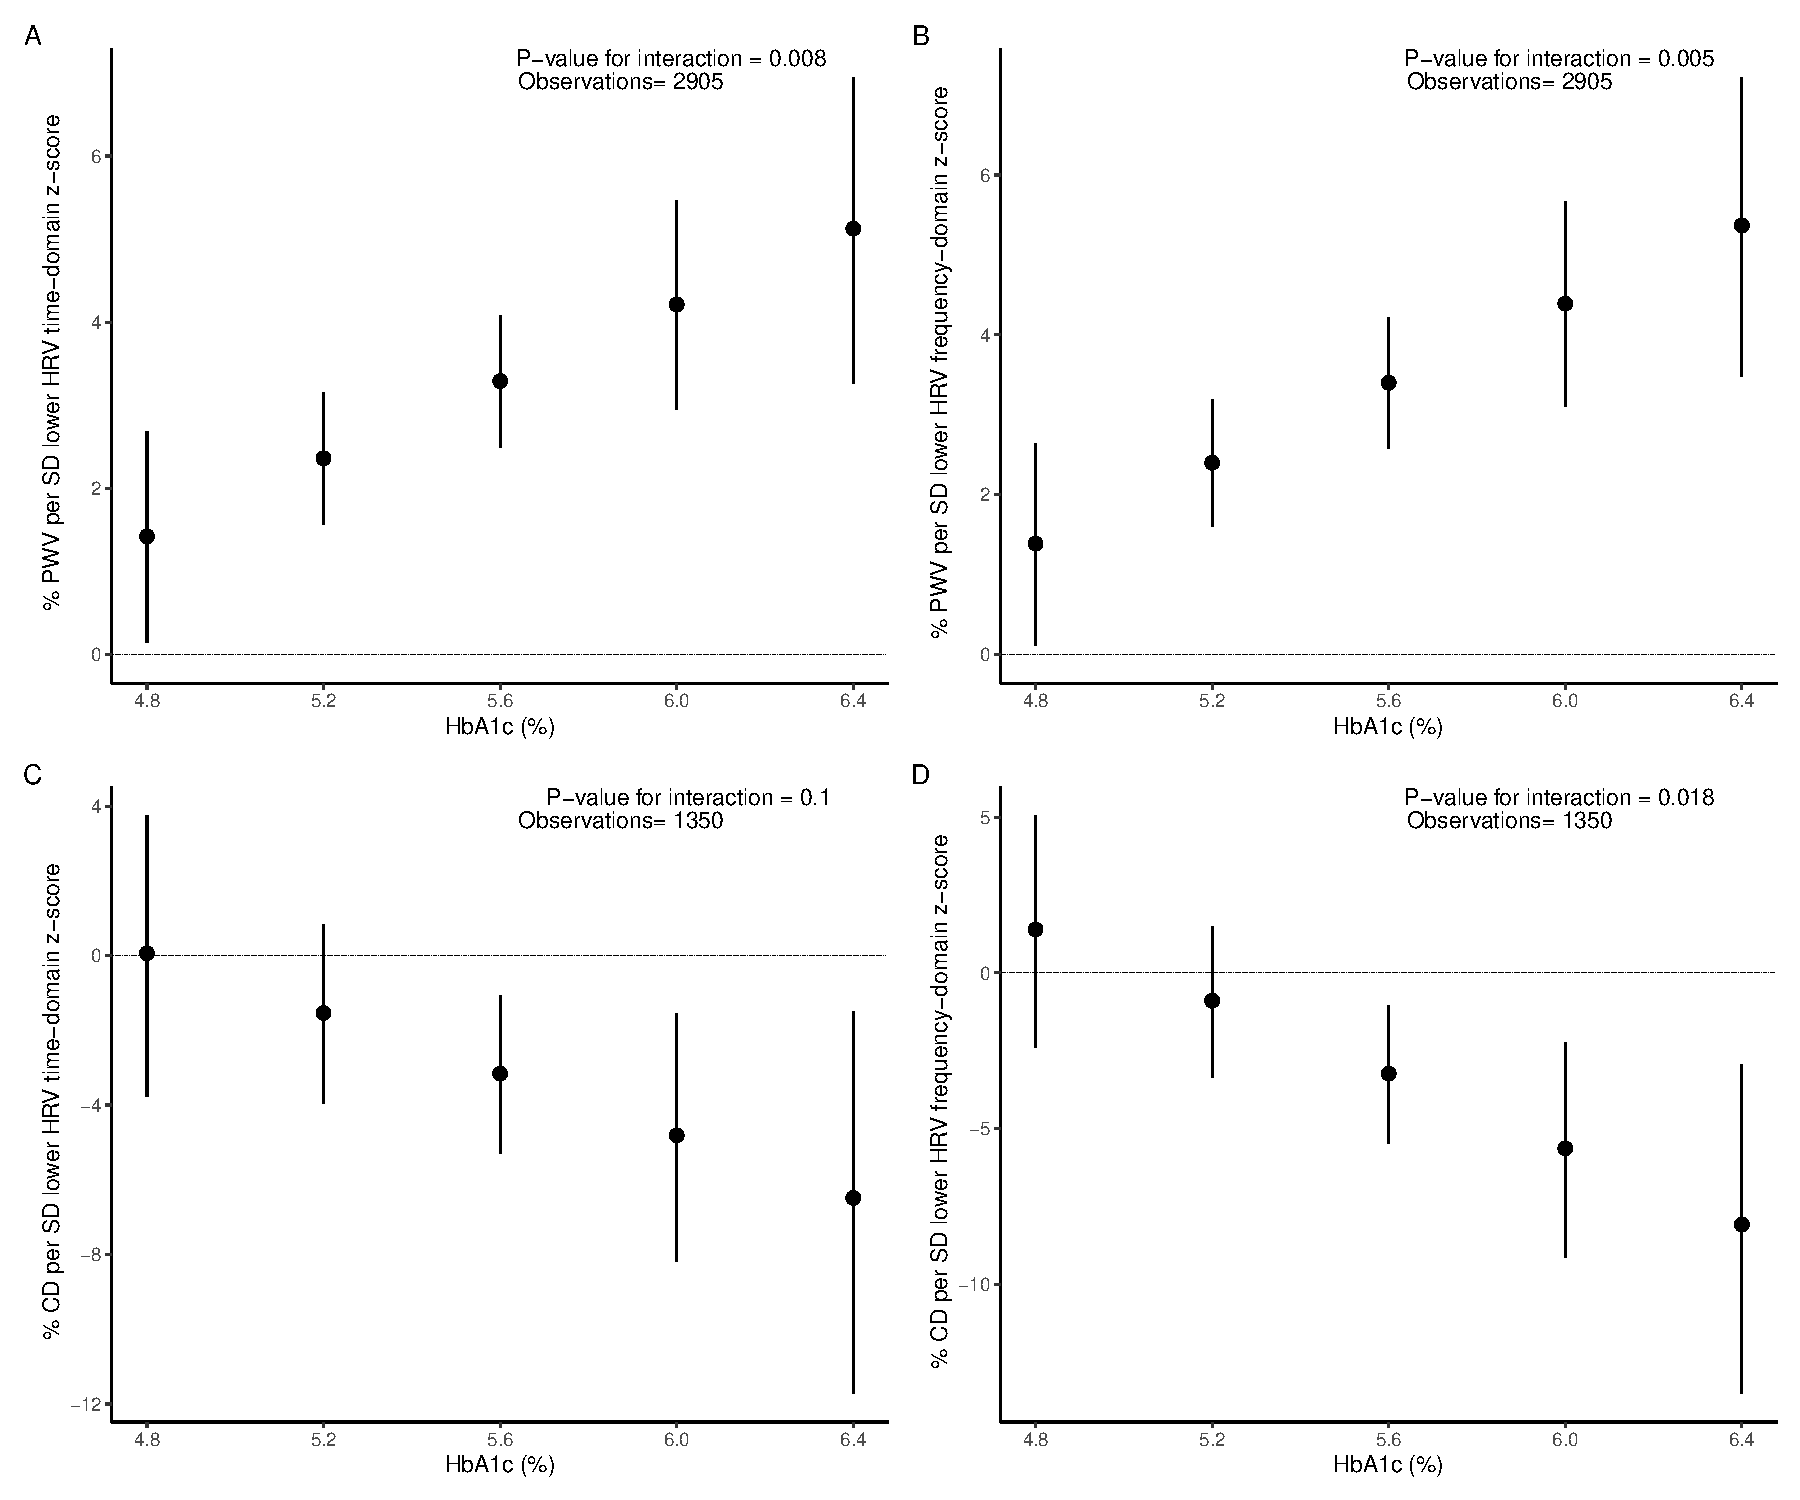
\includegraphics{images/em_hba1c.pdf}

}

\caption{\label{fig-MS-HRV}\textbf{?(caption)}}

\end{figure}

\hypertarget{study-ii}{%
\section{Study II}\label{study-ii}}

\hypertarget{descriptive-1}{%
\subsection{Descriptive}\label{descriptive-1}}

The ADDITION-PRO population consisted of 1,627 participant with a least
48-hour HRV measures, while 1,432 had all hour represented with hourly
HRV and physical acceleration. The study population included different
tiers of diabetes risk: 154 individuals at low risk (9\%), 889 at high
risk (51\%), 314 with impaired fasting glucose (IFG) (18\%), 226 with
impaired glucose tolerance (IGT) (13\%), and 161 with both IFG and IGT
(9\%). I splitted SDNN into categories by very-low (SDNN\textless{} 100
ms), low (SDNN 100-120 ms), middle (SDNN 121-140 ms), high (SDNN 141-160
ms) and very-high (SDNN \textgreater160 ms).

Charteristics are desribed in Table~\ref{tbl-add}. Participants in the
lowest SDNN group (\textless100 ms) were older (67.4 ± 6.9 years), had
higher BMI (28.1 ± 5.4), HbA1c (5.9 ± 0.9), triglycerides (1.5 ± 0.9
mmol/L), and resting heart rate (67.8 ± 5.7 bpm), were more likely to
use anti-hypertensive medication (61\%), and had lower physical activity
energy expenditure (46.8 ± 24.0 kJ/day) compared to those with higher
SDNN levels.

\hypertarget{tbl-add}{}
\begin{table}
\caption{\label{tbl-add}Study participants charteristics }\tabularnewline

\centering
\resizebox{\linewidth}{!}{
\begin{tabular}{l|l|l|l|l|l|l}
\hline
Characteristic
 & Overall, N = 1,625
 & <100, N = 148
 & 100-120, N = 312
 & 120-140, N = 457
 & 140-160, N = 346
 & >160, N = 362
\\
\hline
sex &  &  &  &  &  & \\
\hline
Men & 866 (53\%) & 68 (46\%) & 148 (47\%) & 206 (45\%) & 203 (59\%) & 241 (67\%)\\
\hline
Women & 759 (47\%) & 80 (54\%) & 164 (53\%) & 251 (55\%) & 143 (41\%) & 121 (33\%)\\
\hline
Age (years) & 65.9 (6.8) & 67.4 (6.9) & 65.7 (6.9) & 66.0 (6.7) & 65.5 (6.6) & 66.0 (7.0)\\
\hline
Physical activity energy expenditure (KJ / day) & 53.1 (25.1) & 46.8 (24.0) & 49.4 (21.0) & 50.7 (21.5) & 57.6 (27.2) & 57.5 (29.2)\\
\hline
Alcohol consumption (units per week) & 9.2 (9.5) & 11.3 (10.8) & 10.2 (11.3) & 8.9 (8.5) & 8.5 (9.2) & 8.7 (8.2)\\
\hline
Smoking status &  &  &  &  &  & \\
\hline
1 & 263 (16\%) & 40 (28\%) & 70 (23\%) & 65 (14\%) & 41 (12\%) & 47 (13\%)\\
\hline
2 & 750 (47\%) & 58 (40\%) & 145 (47\%) & 214 (47\%) & 162 (47\%) & 171 (48\%)\\
\hline
3 & 598 (37\%) & 47 (32\%) & 95 (31\%) & 174 (38\%) & 140 (41\%) & 142 (39\%)\\
\hline
BMI (kg/m² & 27.7 (4.7) & 28.1 (5.4) & 28.2 (4.6) & 28.0 (4.7) & 27.7 (4.9) & 26.9 (4.2)\\
\hline
Waist circumference (cm) & 96.7 (13.4) & 98.0 (14.9) & 98.2 (13.2) & 96.7 (13.6) & 96.7 (13.1) & 94.8 (12.5)\\
\hline
Systolic blood pressure (mmHg) & 133.7 (17.3) & 134.2 (16.3) & 133.7 (17.6) & 133.5 (17.8) & 133.4 (16.9) & 133.8 (17.5)\\
\hline
Diastolic blood pressure (mmHg) & 81.9 (10.4) & 83.8 (10.1) & 82.7 (10.2) & 81.7 (10.6) & 82.1 (10.2) & 80.6 (10.3)\\
\hline
Pulse rate (bpm) & 67.4 (10.9) & 77.7 (11.2) & 72.6 (9.3) & 67.9 (9.3) & 65.3 (9.3) & 60.0 (9.8)\\
\hline
HbA1c (\%) & 5.8 (0.5) & 5.9 (0.9) & 5.9 (0.6) & 5.8 (0.5) & 5.7 (0.4) & 5.7 (0.4)\\
\hline
Triglycerides (mmol/L) & 1.3 (0.7) & 1.5 (0.9) & 1.4 (0.7) & 1.3 (0.6) & 1.2 (0.7) & 1.1 (0.6)\\
\hline
Total cholesterol (mmol/L) & 5.4 (1.1) & 5.2 (1.0) & 5.4 (1.2) & 5.4 (1.1) & 5.4 (1.0) & 5.4 (1.0)\\
\hline
HDL cholesterol (mmol/L) & 1.6 (0.4) & 1.6 (0.4) & 1.5 (0.5) & 1.6 (0.4) & 1.6 (0.4) & 1.6 (0.4)\\
\hline
LDL cholesterol (mmol/L) & 3.2 (1.0) & 3.0 (1.0) & 3.2 (1.1) & 3.2 (1.0) & 3.3 (0.9) & 3.3 (0.9)\\
\hline
Urine albumin-creatine ratio (mg/g) & 25.9 (132.8) & 36.4 (105.9) & 47.9 (275.1) & 19.6 (48.2) & 19.4 (67.7) & 16.4 (36.3)\\
\hline
vo2max & 26.6 (7.8) & 24.8 (7.5) & 24.8 (7.5) & 26.1 (6.8) & 27.0 (8.0) & 28.7 (8.7)\\
\hline
rest\_hr & 57.3 (7.3) & 67.8 (5.7) & 63.3 (5.0) & 58.4 (4.5) & 55.0 (4.2) & 49.8 (4.9)\\
\hline
med\_any\_anti\_hypertensive & 753 (47\%) & 88 (61\%) & 149 (48\%) & 216 (47\%) & 147 (43\%) & 153 (43\%)\\
\hline
\end{tabular}}
\end{table}

\hypertarget{multiday-hrv-and-mace-heart-failure-and-all-cause-mortality.}{%
\subsection{Multiday HRV and MACE, heart failure, and all-cause
mortality.}\label{multiday-hrv-and-mace-heart-failure-and-all-cause-mortality.}}

The mean multiday SDNN was 139.0 (32.3) ms, and the mean heart rate was
73.5 (9.1) bpm. In the fully adjusted model, SDNN per SD was associated
with a lower incidence rate ratio (IRR) for MACE 0.82 (CI: 0.69; 0.97),
heart failure 0.76 (CI: 0.58; 0.99), and mortality rate ratio of 0.79
(CI: 0.66; 0.94). When I pre-adjusted for resting heart rate, the
proportion of the association explained between HRV and MACE, HF, and
all-cause mortality was 14\%, 25\%, and 19\%, respectively. I included
knots in the model, which showed that the risk became higher when SDNN
fell below 120 to 110 ms (approximately below the 20th percentile),
suggesting a potential cut-off point for higher risk. I therefore
calculated the incidence rate (IR) at SDNN levels of 100 ms, 120 ms, and
160 ms, respectively, and plotted these as a function of age.

\begin{figure}

{\centering 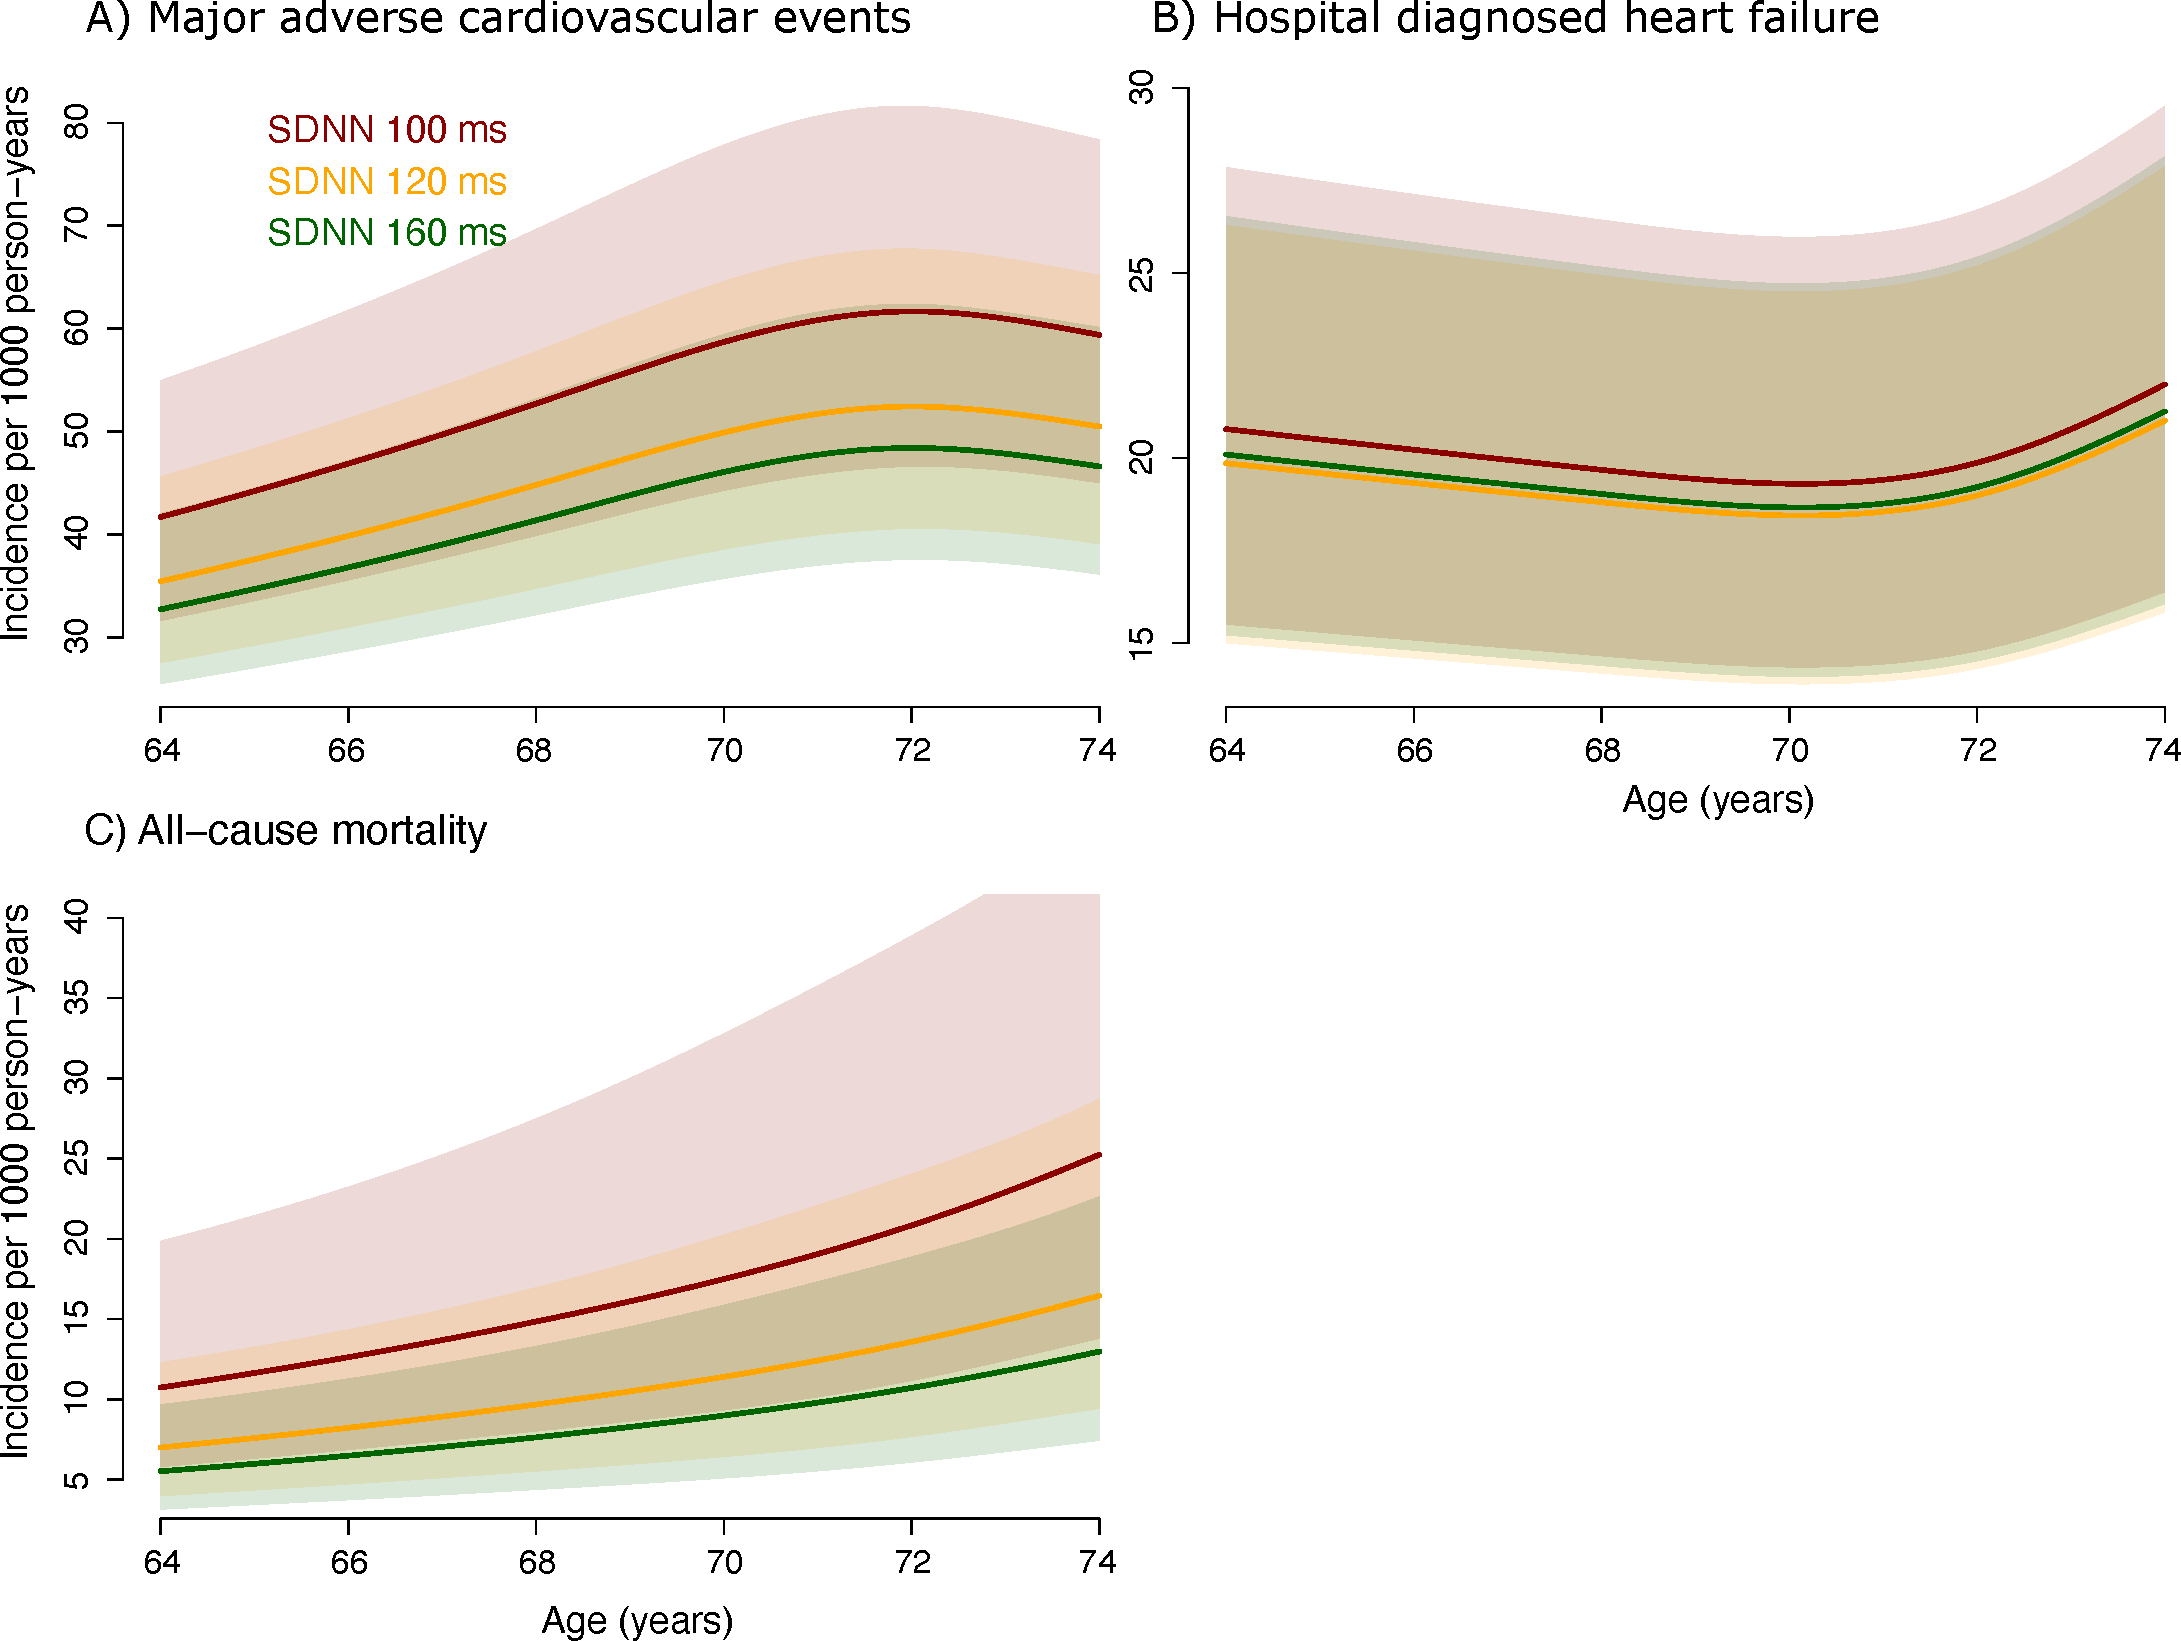
\includegraphics{images/addition_pro_hrv_ir_mace.pdf}

}

\caption{\label{fig-addprohrv}Multiday SDNN levels (100 ms, 120 ms, 160
ms) by age-specific incidence rates for A) major adverse cardiovascular
events, B) heart failure, and C) all-cause mortality}

\end{figure}

At age 65, the IR per 1000 person-years for MACE was 44.2 (CI: 33.5;
58.3) at SDNN = 100 ms, which was higher than the rates observed at SDNN
= 120 ms (IR: 37.6 {[}CI: 29.2; 48.3{]}) and SDNN = 160 ms (IR: 34.7
{[}CI: 27.0; 44.5{]}) (Figure~\ref{fig-addprohrv} A). The IR became
higher with age, reaching its peak at age 72. For heart failure at age
65, the IR was 20.5 (CI: 15.3; 27.5) at SDNN = 100 ms, slightly higher
than at SDNN = 120 ms (IR: 19.6 {[}CI: 14.8; 25.9{]}) and SDNN = 160 ms
(IR: 19.8 {[}CI: 15.0; 26.2{]}) (Figure~\ref{fig-addprohrv} B). The IR
remained stable until age 70, after which it became higher. For
all-cause mortality at age 65, the IR was 11.6 (CI: 6.3; 21.4) at SDNN =
100 ms, higher than at SDNN = 120 ms (IR: 7.6 {[}CI: 4.3; 13.3{]}) and
SDNN = 160 ms (IR: 6.0 {[}CI: 3.4; 10.4{]}) (Figure~\ref{fig-addprohrv}
C). The IR for all-cause mortality became higher with age.

\hypertarget{hourly-hrv-and-mace-heart-failure-and-all-cause-mortality.}{%
\subsection{Hourly HRV and MACE, heart failure, and all-cause
mortality.}\label{hourly-hrv-and-mace-heart-failure-and-all-cause-mortality.}}

From the hourly recordings, I observed a clear periodicity in SDNN,
heart rate, sleep patterns, and physical acceleration. Mean (SD) SDNN
increased from 5--6 AM (70.2 {[}28.8{]} ms), peaking at 8--9 AM (92.1
{[}29.0{]} ms), followed by a gradual decline, reaching its lowest point
around 2 AM the next day (64.1 {[}28.1{]} ms). A similar circadian
pattern was observed in heart rate, although its peak occurred two hours
later, starting at 9 AM (76.7 {[}10.9{]} bpm). After peaking, heart rate
remained stable throughout the afternoon before gradually decreasing.

In Figure~\ref{fig-ADD_PRO_risk_by_hour}, I observe hourly SDNN
(preadjusted for heart rate and physical acceleration), heart rate, and
physical acceleration association. Models was adjusted for age, sex,
education, alcohol consumption, smoking behavior, BMI, total
cholesterol, and Hba1c. The morning response of SDNN was most indicative
of MACE, with the strongest association observed from 6--7 AM (IRR:
0.84; 95\% CI: 0.71 to 1.00 per SD higher SDNN) (see
Figure~\ref{fig-ADD_PRO_risk_by_hour} A).Heart rate between 12 AM and 6
AM showed a small trend toward higher risk of MACE (IRR range: 1.11 to
1.15 per SD higher heart rate), although none of the confidence
intervals exceeded one (see Figure~\ref{fig-ADD_PRO_risk_by_hour} D).
Across all hours, there was a plausible association between SDNN and
heart failure. However, this association disappeared after adjusting for
physical acceleration and heart rate (see
Figure~\ref{fig-ADD_PRO_risk_by_hour} B). In contrast, heart rate
between 10 PM and 9 AM was associated with heart failure (IRR range:
1.37 to 1.58 per SD higher heart rate) (see
Figure~\ref{fig-ADD_PRO_risk_by_hour} E). SDNN was consistently
associated with all-cause mortality across all hours, with a stronger
inverse association observed between 12 PM and 1 AM (IRR range: 0.79 to
0.88 per SD higher SDNN) (see Figure~\ref{fig-ADD_PRO_risk_by_hour} C).
No clear trends of association were observed between heart rate and
all-cause mortality.

\begin{figure}

{\centering 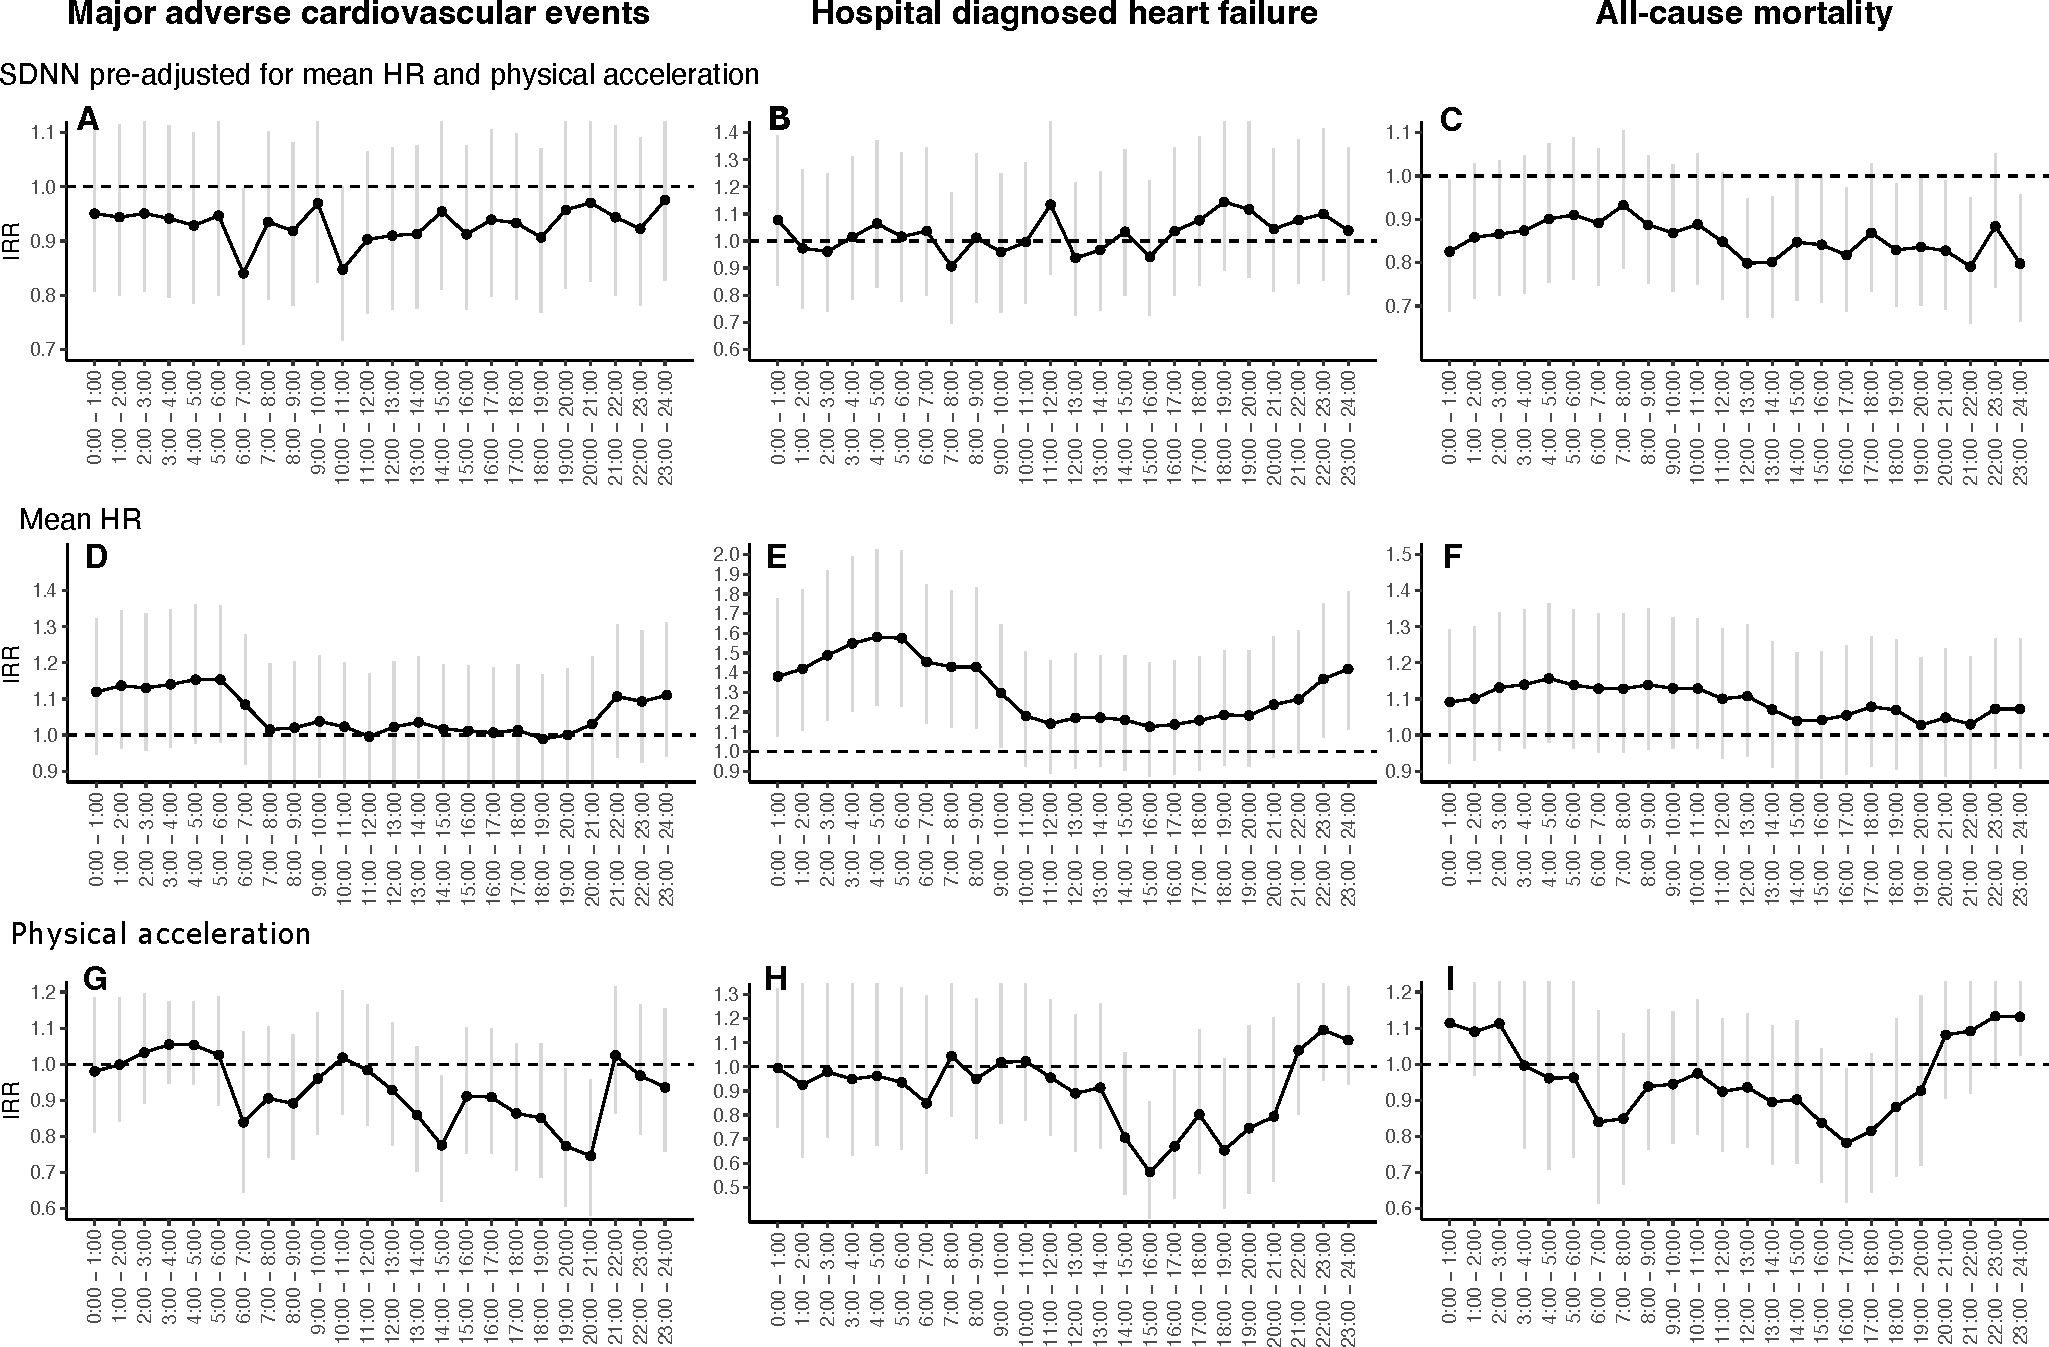
\includegraphics{images/figure_ADD_PRO_risk_by_hour.pdf}

}

\caption{\label{fig-ADD_PRO_risk_by_hour}Hourly SDNN levels (100 ms, 120
ms, 160 ms) by age-specific incidence rates for A) major adverse
cardiovascular events, B) heart failure, and C) all-cause mortality.
Figure adapted from {[}authors{]}. ---. (Paper II, appendix)}

\end{figure}

\hypertarget{study-iii}{%
\section{Study III}\label{study-iii}}

\hypertarget{descriptive-2}{%
\subsection{Descriptive}\label{descriptive-2}}

In study III, 179 participants with type 2 had measures of NT-proBNP and
performed the CART test. CAN was present in 30\% (n = 54) of
participants (36\% among those with valid CAN measurements
(Figure~\ref{fig-CAN} A)). Meanwhile, 24\% (n = 43) were unable to
complete the CART assessment adequately, primarily due to irregular
heart rhythms (n = 8) or insufficient air pressure during the Valsalva
manoeuvre (n = 21). Compare to those without CAN, the participants with
CAN were more women (41 \% vs 33 \%), were more sedentary (45\% vs
36\%), had a higher proportion with prior major CVD (41\% vs 20\%) and
declined eGFR (\textless{} 60) (36\% vs 22\%), higher levels of
triglyceride (median 2.05 mmol/L vs 1.95 mmol/ L), were slightly older
(median 62 years vs 61 years), had longer duration of type 2 diabetes
(median 19 years vs 15 years), and higher use SGTL2-inhibitors (65\% vs
60\%) but lower use of GLP-1 RA (63\% vs 70\%). No other difference in
clinical characteristic was observed.

\hypertarget{can-and-indicators-of-heart-failure}{%
\subsection{CAN and indicators of heart
failure}\label{can-and-indicators-of-heart-failure}}

A greater proportion of individuals with CAN exhibited elevated
NT-proBNP levels (\textgreater125 pg/ml) (51.9\%, n=52/78) compared to
those without CAN (23.2\%, n=26/112)(Figure~\ref{fig-CAN} E). The fully
adjusted odds ratio (OR) for elevated NT-proBNP in individuals with CAN
was 5.69 (95\% CI: 1.95; 18.49) relative to those without CAN. Among the
cardiovascular autonomic reflex tests (CART), the Valsalva maneuver
demonstrated the strongest association with NT-proBNP (OR 9.00, 95\% CI:
2.88; 33.09; n=51/75), followed by deep breathing (OR 3.30, 95\% CI:
1.17; 9.77; n=33/133) and orthostatic hypertension (OR 4.04, 95\% CI:
1.27; 13.77; n=24/146). No significant association was identified for
the lying-to-standing test (OR 0.80, 95\% CI: 0.32; 1.97; n=54/108).
After imputing missing CART data, the OR for CAN in relation to elevated
NT-proBNP declined to 2.94 (95\% CI: 1.37; 6.56). Sensitivity analyses,
which excluded participants using beta-blockers or those with a history
of CVD, resulted in a smaller sample size and wider confidence
intervals, though the overall association remained unchanged. CAN was
associated with elevated NT-proBNP in individuals both without (NYHA I;
OR = 4.3, 95\% CI: 1.1; 16.3) and with heart failure symptoms (NYHA ≥
II; OR = 16.4, 95\% CI: 1.2; 222.0), though the interaction was not
significant (p = 0.4). Similar associations were seen across WATCH-DM
risk groups: very-low-to-moderate (OR = 6.1, 95\% CI: 1.6; 23.5) and
high-to-very-high (OR = 6.3, 95\% CI: 0.83; 46.9). Participants with CAN
had 1.7 (95\% CI: 0.3 to 3.0) point higher WATCH-DM risk score compared
to those without CAN. The OR of presenting with NYHA class II or higher
was 5.51 (95\% CI: 1.9 to 15.97) in the group with CAN.

\begin{figure}

\begin{minipage}[t]{\linewidth}

{\centering 

\raisebox{-\height}{

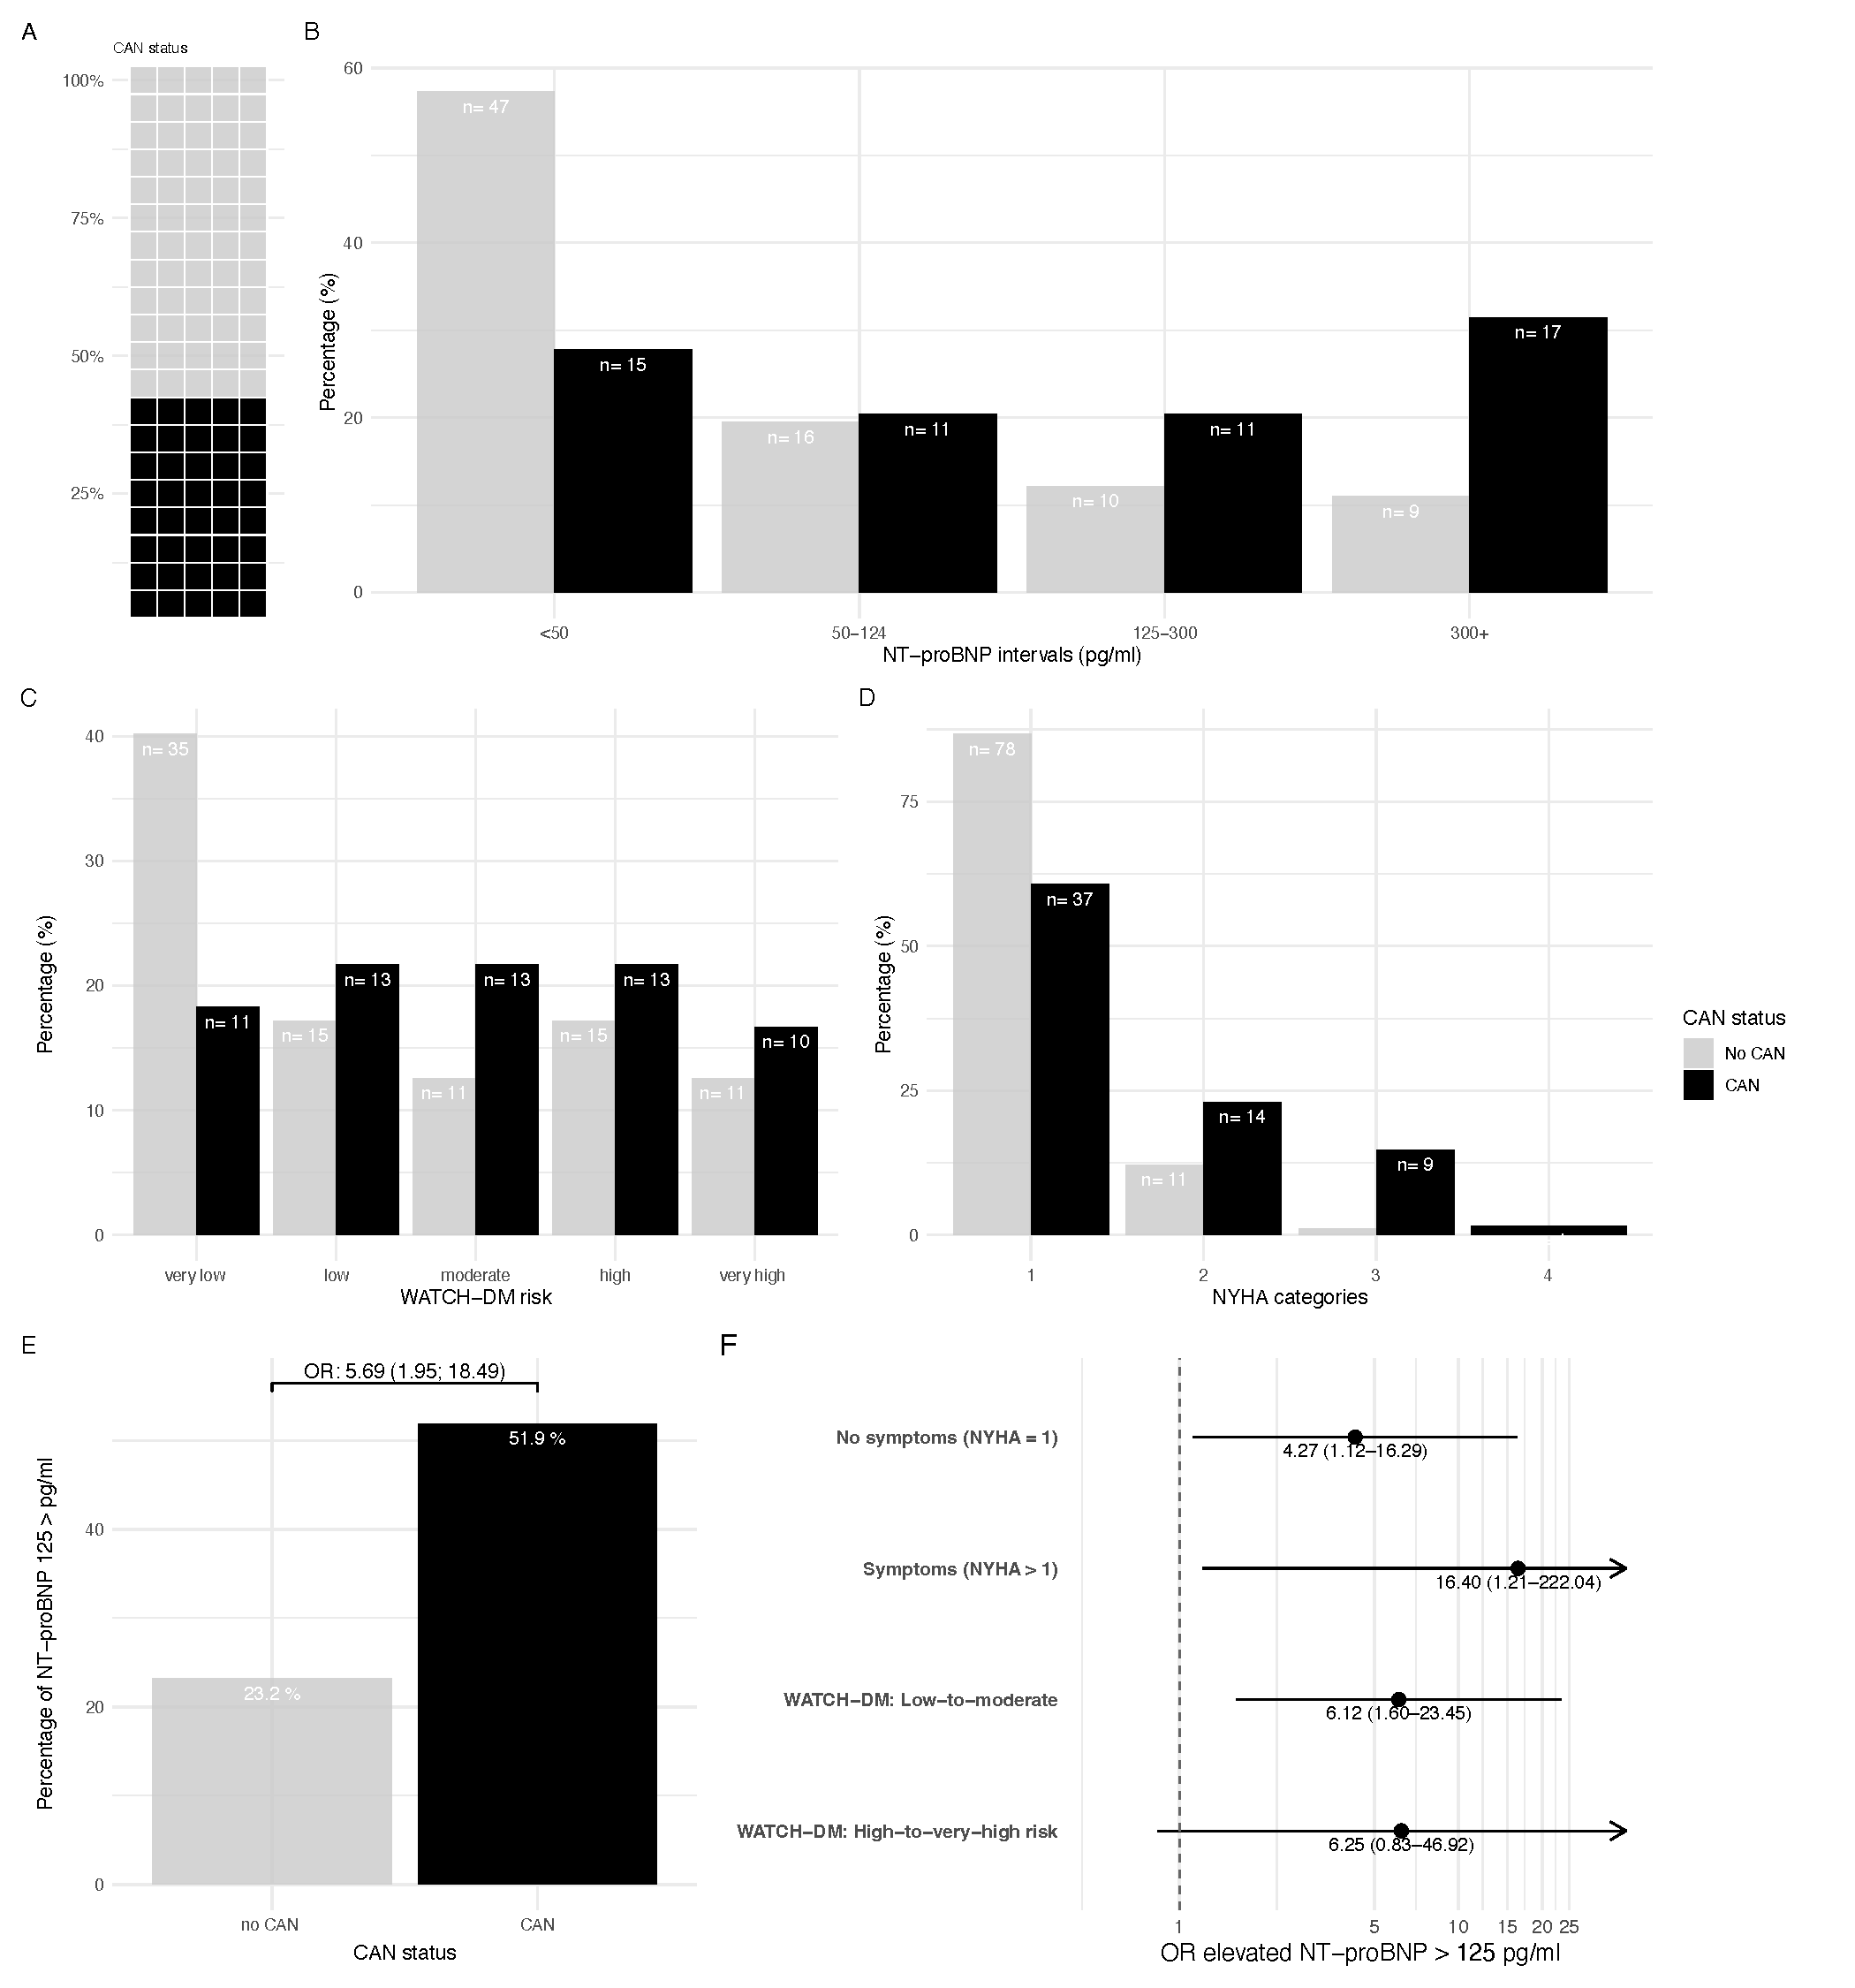
\includegraphics{images/heart_failure_distribution_can_figure_2.pdf}

}

\caption{\label{fig-CAN}Relationship betweeen CAN and indicators for
heart failure. Figure from {[}authors{]}. Cardiovascular autonomic
neuropathy and indices of heart failure in type 2 diabetes: The CANCAN
Study. (Paper III, appendix)}

}

\end{minipage}%

\end{figure}

\bookmarksetup{startatroot}

\hypertarget{discussion}{%
\chapter{Discussion}\label{discussion}}

The aim of this dissertation is to understand how cardiovascular
autonomic dysfunction and CAN affect the risk of CVD across stages of
glucose metabolism. Given the rising prevalence of prediabetes and T2D,
and their association with increased risks of CVD and heart failure,
there is a pressing need for earlier indicators to help healthcare
providers intervene in a timely manner and prevent progression to more
advanced stages of cardiovascular complications. One promising approach
involves leveraging data from wearable devices and standardized
screening tools. Heart rate dynamics and variability across different
circumstances may hold promise as accessible indicators for early
cardiovascular risk stratification.

This chapter presents a summary of the main findings from this
dissertation, interpreted in the context of existing evidence in the
field, and discusses their clinical relevance across different levels of
healthcare. Moreover, the strengths and limitations of the methods and
results will be discussed.

\newpage

\hypertarget{summary-of-findings}{%
\section{Summary of findings}\label{summary-of-findings}}

In this dissertation, autonomic dysfunction, defined by long-term HRV
and standardized CARTs, and its relationship with cardiovascular
complications were studied across three different cohorts representing
populations at varying levels of prevention and care, including public
health, primary care, and secondary care. In the Maastricht study (Study
I), I investigated autonomic dysfunction, measured by 24-hour HRV, and
arterial stiffness, assessed dynamically at the aortic site and locally
at the carotid site among individuals with normal glucose metabolism,
prediabetes, and T2D. Lower HRV was associated with higher aortic and
carotid stiffness. This association was evident regardless of glucose
metabolism status, and was more pronounced in individuals with
prediabetes or T2D. While no significant difference was observed between
prediabetes and T2D, the association was modified by HbA1c after
excluding individuals with T2D, supporting the modifying effect of
dysglycemia. Z-scores of time- and frequency-domain measures showed the
strongest associations, primarily driven by HRV indices reflecting total
variation in interbeat intervals (SDNN, SDANN, SDNN index, ULF, VLF,
TP).

Following Study I, I focused on individuals at higher risk of developing
diabetes, using data from the ADDITION-PRO (Study II) cohort of
individuals representing high-risk individuals of diabetes. In study II,
per lower SD in SDNN, measured over a multiple days, was associated with
18\%, 24\%, and 21\% higher risk for ischemic-related CVD,
hospitalization of heart failure, and all-cause mortality, respectively.
The risk became higher at SDNN levels below 120 ms, supported by a
greater difference in incidence rates between individuals with 100 ms
and 120 ms than the difference observed between individuals with 120 ms
and 160 ms. Hourly measures suggested a specific time point related to
ischemic-related CVD, as lower SDNN recorded between 6:00 and 7:00 AM
was associated with MACE. Residual adjustment of concurrent heart rate
and physical movement did not explain the observed association. Hourly
SDNN was associated with all-cause MRR, although no specific time point
showed an exceptionally strong association. While no association between
hourly SDNN and heart failure was observed, higher heart rate during the
night hours from 02:00 to 06:00 AM was linked to an increased risk of
heart failure hospitalization.

Our findings suggest that both long-term HRV measures and hourly HRV
responses may serve as indicators of CVD risk. However, a key limitation
is that long-term HRV was assessed under free-living conditions, which
restricts the ability to perform standardized tests of autonomic
function. In the CANCAN study (study III), I used standardized CARTs to
define CAN and describe indicators of heart failure, defined by elevated
NT-proBNP, WATCH-DM risk, and NYHA classification among those with and
without CAN in a population with T2D. In CANCAN, two out five had CAN.
Compared to individuals without CAN, theses individual more often showed
signs of heart failure, including elevated NT-proBNP levels, higher
WATCH-DM risk score, and higher classifications on the NYHA. CAN was
association elevated NT-proBNP levels and the persisted even among
individuals without heart failure symptoms based on NYHA classification,
as well as those categorized as having low to moderate heart failure
risk according to the WATCH-DM score.

In summary, various aspects of autonomic dysfunction and cardiovascular
complications were investigated in populations with normal glucose
metabolism, prediabetes, and T2D.The overall findings showed that
autonomic function, assessed through heart rate dynamics of long-term
HRV and diurnal HRV and heart rate responses, is associated with an
increased risk of CVD and heart failure. This relationship appears to be
stronger in more severe stages of dysglycemia. Moreover, among
individuals with T2D, the presence of CAN may help identify those at
higher risk of heart failure, even in the absence of heart failure
symptoms.

\hypertarget{cardiovascular-autonomic-dysfunction-and-its-impact-on-heart-disease-across-glucose-metabolism}{%
\section{Cardiovascular autonomic dysfunction and its impact on heart
disease across glucose
metabolism}\label{cardiovascular-autonomic-dysfunction-and-its-impact-on-heart-disease-across-glucose-metabolism}}

This dissertation show that cardiovascular autonomic dysfunction,
measured by HRV and CARTs, is associated with CVD risk across the
spectrum of glucose metabolism dysregulation. This association is
evident with measures of arteriosclerosis, atherosclerotic events,
all-cause mortality, and heart failure in individuals at high risk of
diabetes, as well as with indications of heart failure in patients with
T2D.

\hypertarget{arteriosclerosis-1}{%
\subsubsection{Arteriosclerosis}\label{arteriosclerosis-1}}

In Study I, autonomic dysfunction, measured by 24-hour HRV, showed to be
associated with arterial stiffness, assessed both dynamically (cf-PWV)
and locally (CD). This suggests that autonomic responses under
free-living conditions contribute to the development of arterial
stiffness. Majority of studies have shown an association between
autonomic dysfunction, as measured by short-term HRV during rest, and
arterial stiffness in populations with either type 1 or
T2D\textsuperscript{62}. Study I extended this perspective by long-term
HRV and including a population without diabetes or prediabetes.

\begin{figure}

{\centering 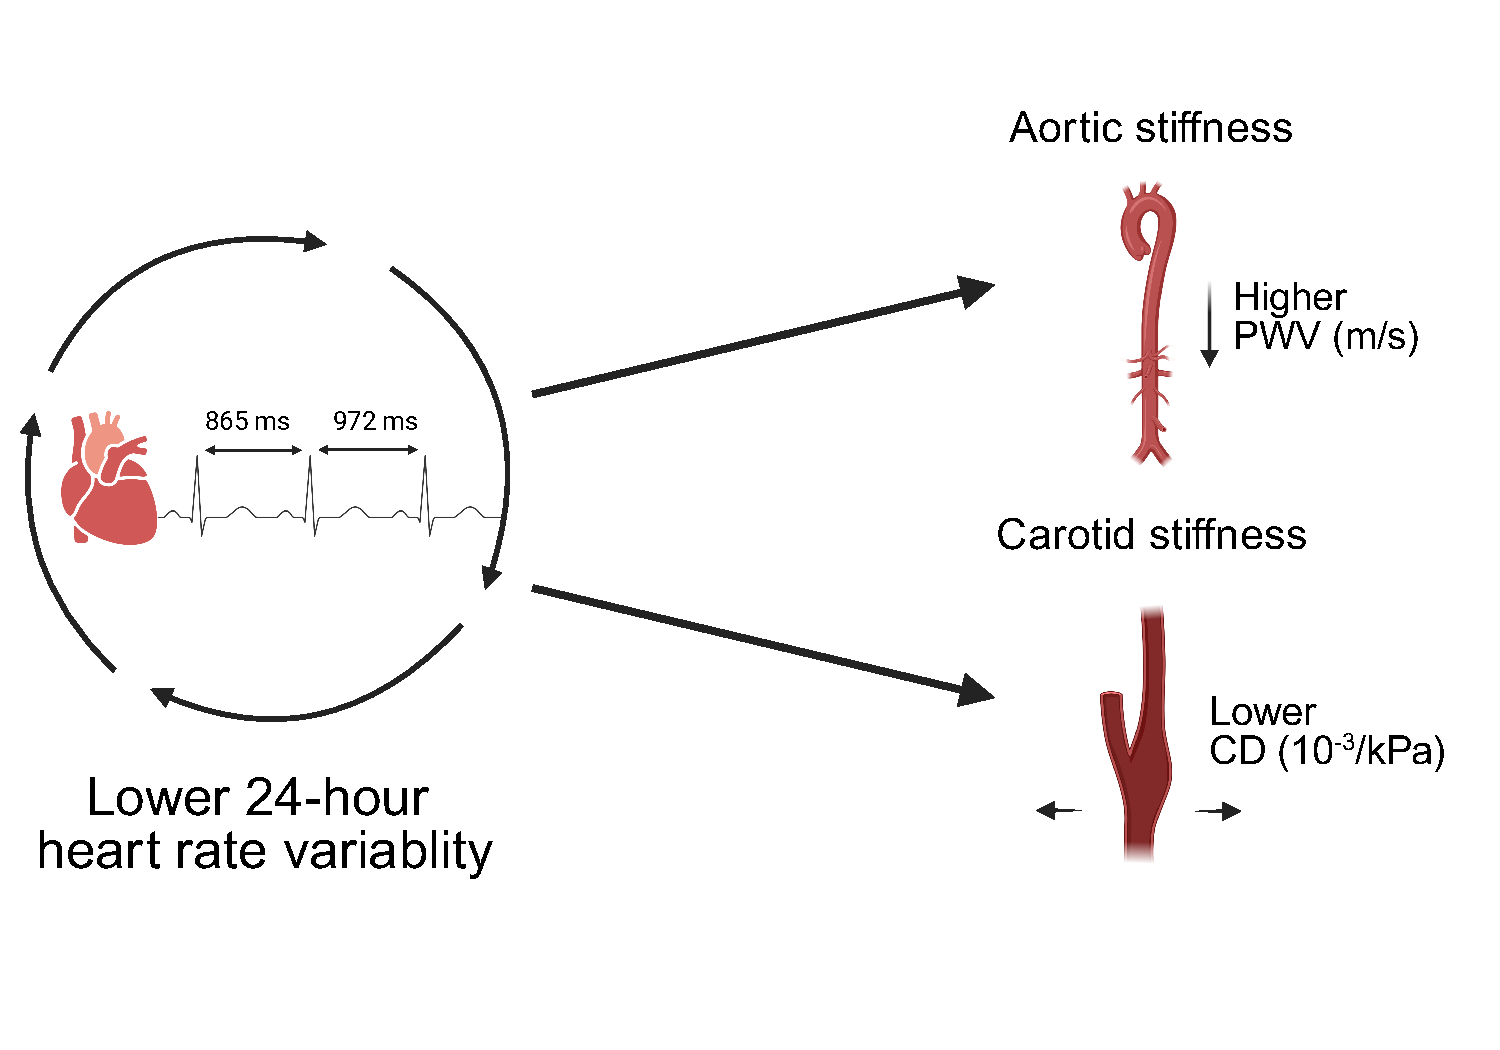
\includegraphics[width=4in,height=\textheight]{images/hrv_arterial_stiffness.pdf}

}

\caption{Autonomic dysfunction and arterial stiffness. (Source: Author).
---.}

\end{figure}

Arterial stiffness is not only a structural marker of vascular ageing
but is also dynamically modulated by local endothelial signals and
autonomic nervous system activity. Several studies have demonstrated a
link between elevated sympathetic tone and increased arterial
stiffness{[}\textsuperscript{63}{]}\textsuperscript{64}. Two possible
mechanisms may explain how autonomic dysfunction is related to arterial
stiffness. First, autonomic dysfunction may increase the vascular tone
of large arteries, thereby impairing arterial elasticity. This concept
is supported by animal studies. In rats, proper autonomic regulation has
been shown to be essential for maintaining aortic elasticity.
Conversely, chronic overstimulation of sympathetic activity can lead to
structural remodeling and increased arterial stiffness. Therefore,
although the initial effects of autonomic dysfunction are dynamic and
amenable to change by intervention, they may become progressively less
reversible over time. While such findings cannot be directly
extrapolated to humans, they suggest plausible biological pathways.
Second, the autonomic nervous system regulates heart rate and cardiac
contractility. Autonomic dysfunction typically manifests as both reduced
HRV and elevated resting heart rate. Arterial shear stress increases as
a result of heightened sympathetic activity and parasympathetic
withdrawal. A higher resting heart rate may contribute to structural
stiffer arteries by altering blood flow dynamics and increasing shear
stress. Our earlier study using data from the Whitehall II cohort showed
that a steeper decrease in short-term (5-minute) HRV over a ten-year
period was linked with higher levels of aortic stiffness in the
subsequent five years\textsuperscript{65}.

The association between 24-hour HRV and arterial stiffness was modified
by dysglycemia, suggesting dysclycemia introduce CAN that can affect
arterial stiffness, even before the onset of
T2D{[}\textsuperscript{66}{]}\textsuperscript{67}\textsuperscript{68}.
Data from the Whitehall II study showed that aortic stiffness increased
more steeply with higher HbA1c values among non-diabetic
individuals\textsuperscript{69}. In the subpopulation in Study I without
diabetes, a modification by HbA1c in both aortic and carotid stiffness
was observed. The modifying effect of HbA1c suggests that hyperglycaemia
amplifies the consequences of autonomic dysfunction.

\hypertarget{atherosclerosis-1}{%
\subsubsection{Atherosclerosis}\label{atherosclerosis-1}}

In Study II, I showed that individuals with a preclinical stage of
autonomic dysfunction, measured by multiday HRV, face a higher risk of
incident ischemic CVD, heart failure, and all-cause mortality.

We assessed week-long HRV to capture autonomic activity in real-life
settings across several days. Our results are consistent with earlier
research linking reduced HRV to cardiovascular outcomes and
mortality\textsuperscript{5}. Our findings build on existing evidence by
(1) focusing on a population at elevated risk of diabetes, (2) utilizing
multiday HRV recordings, and (3) identifying specific daily periods
where HRV patterns were indicative of ischemic-related CVD risk. By
using both week-long and hourly data, we identified specific periods of
higher risk. A strength of using multiday HRV recordings, is to provide
more robust insights into individual autonomic patterns by averaging
cardiovascular responses across typical daily conditions. This reduces
the influence of random fluctuations caused by factors such as physical
activity, emotional states, or sleep on any single
day\textsuperscript{70}.

Multiple mechanisms may explain how autonomic dysfunction contributes to
the initiation and progression of ischemic events and stroke. First, as
discussed in Study I, autonomic dysfunction may promote
arteriosclerosis, leading to arterial stiffness through a dynamic and
potentially modifiable process. Arterial stiffness impairs vasodilation,
increasing hemodynamic stress and the risk of plaque rupture and
thrombus formation {[}\textsuperscript{71}{]}\textsuperscript{72}. In
this context, findings from Study I may not entirely distinguish between
arterial stiffness and atherosclerosis, as shown by data from the
Rotterdam Study\textsuperscript{73}. As plaques develop, the associated
increase in sympathetic nerve density around the arteries could
transiently reduce vascular tone which over time reduce arterial
elasticity\textsuperscript{74}. In a smaller study of people with T2D,
lower HRV was linked with increased carotid
atherosclerosis\textsuperscript{75}.

Second, the autonomic nervous system innervates the adventitia layer of
blood vessels, where it modulates vascular tone via sympathetic fibres.
Although atherosclerotic plaques form in the intima layer, recent in
vivo studies have demonstrated that increased plaque burden is
associated with higher local sympathetic nerve density, likely mediated
by neuroinflammatory processes. Notably, reducing sympathetic
innervation has been shown to attenuate plaque formation in animal
models\textsuperscript{76}. These findings suggest that autonomic
dysfunction may not only reflect but also actively contribute to
atherogenesis.

Third, autonomic nervous dysfunction has been shown to interfere with
signalling pathways controlling heart rhythm, potentially leading to
arrhythmias that disturb cardiac contraction. Data from the
Atherosclerosis Risk in Communities study illustrated that lower
short-term HRV was associated with incident atrial fibrillation over 20
years, with a higher risk among participants with
T2D\textsuperscript{77}. This supports the role of autonomic dysfunction
in arrhythmogenesis, which increases the risk of myocardial infarction
and stroke. However, in Study II, I did not include incident atrial
fibrillation as an outcome. We did not include atrial fibrillation as an
outcome in Study II due to limitations in Danish registries, which often
do not distinguish between short- and long-term AF, affecting diagnostic
validity. Future research is needed to explore whether it could explain
the higher risk of major adverse cardiovascular events.

A study of individuals with coronary artery disease showed that
stress-induced HRV was associated with myocardial infarction, even more
than resting HRV, suggesting that reduced parasympathetic modulation of
heart rate under stress may play a role in ischemia\textsuperscript{78}.
Our study focused on long-term HRV under free-living conditions,
capturing stress-responsive periods such as morning awakening. These
recordings likely reflect underlying autonomic dynamics relevant to
cardiovascular risk. A Genome-Wide Association Study (GWAS) in the UK
biobank of short-term HRV support this by identifying mechanisms
involving G-protein signaling, pacemaker activity, and mitochondrial
function. These pathways influence vagal control, cardiac excitability,
and energy metabolism\textsuperscript{79}. Although derived from
short-term recordings, the genetic associations may reflect autonomic
traits that persist across different time scales, thereby reinforcing
the biological basis of HRV. A Mendelian randomization study using data
from the Rotterdam Study found that genetically predicted HRV was
associated with an increased risk of atrial
fibrillation\textsuperscript{80}. However, this association did not
extend to all-cause mortality or cardiovascular death in the UK Biobank
cohort, where only phenotypically measured HRV showed a significant
relationship with these outcomes\textsuperscript{81}. Interestingly, the
genetic determinants of HRV exhibited pleiotropic relationships with
several autonomic traits, including resting heart rate, heart rate
response during exercise, and post-exercise recovery
dynamics\textsuperscript{81}. No GWAS has been conducted for long-term
HRV. Therefore, it is unclear whether the genetic influences identified
for short-term HRV are applicable to long-term HRV. Future GWAS efforts
targeting long-term HRV could help establish causal relationships by
leveraging methods such as Mendelian randomization, thereby advancing
our understanding of the genetic architecture underlying autonomic
regulation.

\hypertarget{heart-failure-1}{%
\subsubsection{Heart failure}\label{heart-failure-1}}

The relationship between cardiovascular autonomic dysfunction and heart
failure is complex\textsuperscript{82}. On one hand, autonomic
dysfunction contributes to cardiac remodelling and eventual heart
failure. On the other hand, it may reflect compensatory mechanisms of
the progression of cardiac remodelling and declining cardiac output. Our
findings demonstrated a relationship between autonomic dysfunction and
heart failure both cross-sectionally in a population with T2D and
prospectively in individuals representing different tiers of diabetes
risk. However, our data are limited in determining the extent to which
this relationship supports one explanation over the other, as we lack
baseline and follow-up measures of both heart failure and HRV. Earlier
studies have demonstrated that both short-term and long-term HRV are
associated with incident heart failure in populations with and without
T2D.{[}\textsuperscript{83}{]}\textsuperscript{84}{[}\textsuperscript{85}{]}\textsuperscript{86}.
Beyond examining a population at elevated risk of diabetes using
multiday HRV recordings, we expanded previous research by (1) unmasking
the role of resting heart rate in the relationship between HRV and heart
failure risk, and (2) identifying specific times of day when heart rate
patterns signaled higher risk of heart failure.

Several mechanisms may underlie the role of autonomic dysfunction in
advancing heart failure. Findings from Study I confirmed the
relationship between autonomic dysfunction and arterial stiffness. It is
well established that arterial stiffness is linked to cardiac
remodelling, as increased cf-PWV leads to an earlier return of the
reflected pulse wave to the aorta, which increases cardiac afterload and
reduces coronary perfusion pressure\textsuperscript{87}. Therefore,
autonomic dysfunction may have an indirect effect on heart failure,
potentially mediated by arterial stiffness. However, structured analyses
are needed to confirm these pathways. For example, through mediation
analysis to assess the direct and indirect effects of arterial
stiffness, with autonomic dysfunction as the main determinant. In Study
II, I observed that multiday HRV was associated with incident heart
failure, and approximately one-fourth of the risk was explained by
resting heart rate. Data from the Rotterdam Study showed that short-term
HRV was longitudinally associated with echocardiographic measures
reflecting systolic function, suggesting that autonomic dysfunction
contributes to cardiac remodelling\textsuperscript{88}. In contrast to
MACE outcomes, findings from Study II showed no specific time point in
hourly HRV that was associated with heart failure. Instead, it was the
overall daily pattern captured by multiday HRV that was linked to heart
failure risk. This suggests that the association is not driven by
isolated shifts in autonomic activity, but rather by a consistently
impaired autonomic balance under free-living conditions. The effect
appears to be driven in part by a failure to show appropriate decreases
in heart rate during rest, as individuals with higher hourly heart rates
at night had an increased risk of heart failure. In Study III, I
observed that individuals with CAN had higher risk of elevated levels of
NT-proBNP, a biomarker of myocardial stress and early heart failure.
Therefore, CAN is associated with hemodynamic consequences that
contribute to both structural and functional cardiac remodeling, which
in turn leads to elevated NT-proBNP levels.

We cannot exclude the possibility that autonomic dysfunction represents
an elevated demand for compensatory mechanisms as heart failure
progresses. Studies have shown that patients with heart failure and
lower HRV tend to have a worse prognosis in terms of mortality. If low
HRV or the presence of CAN were primarily driven by existing cardiac
complications, it would suggest that individuals with these conditions
exhibit more pronounced sympathetic overactivity as a consequence of
heart failure progression, indicating potential reverse causation.
Hence, elevated sympathetic activity during rest may reflect a greater
reliance on compensatory mechanisms to maintain cardiac output. More
precise measures are needed to assess whether sympathetic activity acts
as a primary driver of heart failure or as a secondary compensatory
response to cardiac dysfunction. In addition, it remains unclear to what
extent the parasympathetic nervous system can act as a protective
mechanism to counterbalance sympathetic dominance, and whether a decline
in HRV reflects a breakdown of this balance. The two pathways (autonomic
neuropathy and cardiac remodelling) are not mutually exclusive and may
interact in a reinforcing cycle. Autonomic dysfunction can lead to
increased sympathetic tone and reduced parasympathetic modulation,
placing the heart under chronic stress and promoting structural and
functional changes\textsuperscript{23}. In turn, cardiac remodelling may
impair autonomic regulation, further exacerbating the imbalance. This
interplay may create a self-perpetuating loop that accelerates the
progression of heart failure. However, this remains beyond the scope of
our current data and analysis.

\hypertarget{clinical-implications}{%
\section{Clinical implications}\label{clinical-implications}}

The dissertation investigates autonomic dysfunction in populations
ranging from normal glucose metabolism to T2D and yields insights
relevant for individuals engaged at different levels of the healthcare
system. No specific role has yet been defined for autonomic dysfunction
in clinical decision-making within healthcare, as current treatment and
intervention options remain limited. Despite the fact that the results
do not extend to the implementation of autonomic dysfunction in clinical
practice, the findings from three included cohorts representing
populations under public health, primary care, and secondary care. They
mark a notable first step in addressing the impact of autonomic
dysfunction on cardiovascular complications. In following section, the
clinical implications of using autonomic dysfunction in the prevention
of CVD will be discussed. If long-term HRV or CARTs are to be considered
for improving risk stratification, it is important to determine at what
stage in the progression of diabetes risk, and at which level of care,
autonomic dysfunction becomes meaningful for early detection and
intervention.

\hypertarget{public-health}{%
\subsection{Public health}\label{public-health}}

A central strategy in preventing CVD is the early identification and
treatment of individuals at high risk\textsuperscript{89}. Public health
initiatives support this by promoting healthy lifestyles, facilitating
early screening for risk factors, and improving access to essential care
and medications. Long-term HRV may enhance these efforts by identifying
individuals with elevated cardiovascular risk and by tracking their
physiological response to lifestyle changes.

Evidence from Study I showed that lower long-term HRV was associated
with increased arterial stiffness, as measured by cf-PWV and CD, even in
individuals without T2D. One standard deviation lower HRV corresponded
to the effect of 2.7 additional years on cf-PWV and 1.6 years on
CD\textsuperscript{90}. These cross-sectional findings suggest that HRV
may serve as a marker of early vascular aging and cardiovascular risk.
Supporting this, the Whitehall II study demonstrated a longitudinal
relationship between short-term HRV and aortic stiffness. Together,
these findings highlight the potential of HRV as a dynamic indicator of
vascular health.

Within the public health setting, individuals with prediabetes represent
a particularly vulnerable group at risk for
comorbidities\textsuperscript{91}. They often fall between structured
care pathways, sometimes receiving regular follow-up and other times
remaining outside formal healthcare systems. Notably, Studies I and II
demonstrated that the associations between long-term HRV and CVD risk
were especially pronounced in this population. In those at high risk of
diabetes, a one standard deviation (33 ms) decrease in multiday SDNN was
equivalent to 4.5 additional years of aging for major adverse
cardiovascular events and 2.2 to 2.4 years for heart
failure\textsuperscript{92}. On a population level, lower HRV (SDNN: 100
ms) in individuals with prediabetes was associated with a higher
incidence rate of CVD, heart failure, and all-cause mortality compared
to individuals with normal-to-higher HRV (SDNN: 120--160 ms). These
findings reinforce the role of HRV as an early and sensitive marker of
cardiovascular health in populations at cardiometabolic risk.

While these findings highlight HRV's potential, practical implementation
faces several challenges. Historically, long-term HRV monitoring has
required specialized equipment such as Holter ECG recorders. However,
the growing popularity of wearable devices offers a promising
alternative. These devices provide a non-invasive, user-friendly way to
collect heart rate and HRV data over time\textsuperscript{11}.

If HRV monitoring proves effective in helping individuals maintain a
healthy, age-adjusted HRV range through lifestyle changes and prompts
healthcare engagement when HRV deteriorates, it could become a
meaningful tool for long-term health tracking. A cross-sectional study
of 8 million individuals found that those who took more steps per day
had higher HRV\textsuperscript{13}, suggesting that HRV may also reflect
behavioral adaptation.

A major public health challenge lies in ensuring equitable access to
wearable technology. Individuals from lower socioeconomic backgrounds
are significantly less likely to own such devices, raising concerns
about health disparities. Despite this, there is encouraging evidence
that the general population is receptive to digital health innovations.
Many are willing to share health data with public institutions and
support the use of AI in disease
monitoring{[}\textsuperscript{11}{]}\textsuperscript{93}.

Integrating wearable HRV monitoring into public health strategies could
represent a transformative step in proactive cardiovascular care. It may
support early detection, personalized prevention, and timely referral to
primary care when risk levels increase.

\hypertarget{primary-care}{%
\subsection{Primary care}\label{primary-care}}

Cardiovascular risk in primary care is assessed using clinical
evaluations and standardized risk prediction tools to identify
individuals at elevated risk (ref.). Management focuses on lifestyle
modification, pharmacological therapy, and regular monitoring to reduce
cardiovascular events (ref.). In this context, long-term HRV may offer
added value by improving the precision of cardiovascular risk
stratification and by serving as a marker to monitor the effectiveness
of preventive strategies.

Long-term HRV may enhance individual risk classification when added to
established clinical risk scores. Tools such as SCORE2 and the
Framingham Risk Score are widely used in primary care to guide
cardiovascular risk assessment\textsuperscript{94,95}. In Study I,
models adjusted for conventional CVD risk factors supported the
potential added value of 24-hour HRV in relation to arterial stiffness,
a surrogate marker of CVD risk. Study II extended this perspective by
demonstrating associations between multiday HRV and incident CVD and
heart failure. However, these findings are based on associations and do
not include formal prediction modeling\textsuperscript{96}. A limitation
of our studies is that we did not evaluate whether incorporating
long-term HRV or CARTs into existing risk scores improves predictive
performance beyond current guidelines. While most biomarkers have shown
limited incremental value beyond established predictors (including age,
sex, lipid profiles, diabetes status, and blood pressure), some studies
suggest that 24-hour HRV may improve risk discrimination for CVD and
all-cause mortality in individuals with T2D\textsuperscript{97}, and for
stroke and heart failure in older
adults{[}\textsuperscript{83}{]}\textsuperscript{98}. However, these
studies often lack calibration or validation in large-scale cohorts and
have not been integrated with widely used risk scores such as SCORE2 or
the Framingham Risk Score.

Long-term HRV may also help identify preclinical autonomic dysfunction,
enabling targeted interventions in a subgroup of patients to prevent
CVD. The increasing availability of wearable devices capable of
capturing long-term HRV data presents a practical opportunity for
continuous monitoring in primary care. These devices may facilitate
earlier detection of autonomic dysfunction and support more personalized
approaches to cardiovascular risk management. However, the clinical
utility of stratifying patients based on preclinical autonomic
dysfunction remains uncertain. These considerations are only actionable
if interventions in this subgroup can be shown to reduce cardiovascular
risk. Emerging evidence suggests that both pharmacological and lifestyle
interventions can improve HRV in the short term\textsuperscript{99,100}.
For example, high-intensity interval training has been shown to improve
autonomic function in obese individuals with and without
T2D\textsuperscript{101}. Similarly, lifestyle changes in individuals
with prediabetes have been associated with improvements in short-term
HRV, which may partly explain a reduction in diabetes risk independently
of weight loss\textsuperscript{102}. Nevertheless, it remains unclear
whether these effects on HRV are sustainable over time and whether they
translate into long-term cardiovascular protection. In many cases,
improvements in autonomic function may be mediated indirectly through
changes in cardiometabolic markers such as glucose levels, lipid
profiles, body weight, maximal oxygen uptake, and blood pressure.

Despite these uncertainties, monitoring autonomic function through
long-term HRV may offer a valuable tool for assessing cardiovascular
risk and tracking the impact of preventive strategies. In Denmark,
prediabetes, defined by HbA1c, is present in 7.1\% of
adults\textsuperscript{103}. One in five of these individuals develops
T2D within five years\textsuperscript{103}, while others either remain
in the prediabetic stage or return to normoglycemia. Despite their
increased risk of CVD and heart failure\textsuperscript{104},
individuals with prediabetes are not captured by existing preventive
strategies. This underscores the need for early and precise risk
assessment\textsuperscript{10}. Given that the cardiovascular
consequences of autonomic dysfunction appear to be more pronounced in
individuals with prediabetes compared to those with normoglycemia, HRV
has the potential to help identify those at elevated CVD risk within
this group. However, evidence demonstrating improved risk prediction and
sustained effects leading to better cardiovascular outcomes is needed to
establish its relevance for integration into primary care.

\hypertarget{secondary-care}{%
\subsection{Secondary care}\label{secondary-care}}

In secondary care, endocrinologists assess cardiovascular and heart
failure risk by integrating advanced diagnostics, biomarker analysis,
and imaging to detect early dysfunction. The treatment of patients with
T2D is guided by evidence-based therapies and multidisciplinary
collaboration. The ADA/EASD 2022 consensus on Management of
Hyperglycemia in T2D emphasizes that early detection of heart failure in
individuals with T2D is crucial, as it enables timely initiation of
therapies such as SGLT2 inhibitors, which have demonstrated significant
benefits in reducing heart failure-related
outcomes\textsuperscript{105}. A major challenge in diabetes care is
detecting heart failure before symptoms appear, as patients with
symptomatic heart failure face a higher risk of mortality and more
frequent hospitalizations\textsuperscript{4}. The AHA, ACC, and HFSA
2022 guidelines recommend identifying individuals at risk of heart
failure based on factors such as diabetes, poor glycaemic control,
uncontrolled hypertension, hyperlipidaemia, elevated BMI, albuminuria,
renal dysfunction, and a history of CVD\textsuperscript{106}. Still,
there is a need to identify optimal approaches for recognizing and
diagnosing heart failure in clinical care, as broad echocardiographic
screening in T2D is time-consuming and costly\textsuperscript{4}.

Study III demonstrated that CAN may help identify individuals at
increased risk of heart failure, beyond what is captured by symptoms or
existing risk scores. Our findings support considering CAN as a relevant
risk factor for heart failure and suggest it may have value in future
risk stratification strategies in T2D. A clinical advantage of using
CARTs is that they are standardized tests performed under controlled
conditions. CARTs has proven to be reliable and reproducible, with
reference values established in large population
studies\textsuperscript{47}. Beyond these findings and the established
evidence of increased heart failure risk, CAN in the T2D population also
identifies individuals at high risk for overall CVD, kidney disease, and
early mortality. In Study III, I observed that two out of five
participants had CAN, highlighting it as a prevalent complication.
Therefore, detecting CAN may uncover an often-overlooked condition that
is common in individuals with T2D.

Clinical stratification of care includes two key considerations: (1) CAN
should be further evaluated for associated cardiovascular complications,
such as heart failure; and (2) cardiopreventive strategies should be
initiated earlier in this subgroup.

First, patients with CAN may benefit from further cardiovascular
assessment, including the use of sensitive biomarkers or
echocardiography. NT-proBNP is a strong predictor of heart failure and a
validated biomarker for ruling out the condition (ref.). However, its
specificity varies across heart failure phenotypes, being less specific
for detecting HFpEF compared to HFrEF. Therefore, additional evaluation
using echocardiography may be warranted. Beyond classify heart failure
phenotypes, echocardiography identifies preclinical stages of heart
failure through the detection of functional or structural cardiac
abnormalities. Including CAN in structured assessments of heart failure
could help clarify to which extent does CAN overlap with cardiac
abnormalities. Determining the diagnostic and prognostic value of CAN,
particularly its sensitivity and specificity in detecting HFrEF and
HFpEF, requires further investigation.

Second, the presence of CAN may justify earlier initiation of protective
therapies. SGLT2 inhibitors are recommended as second-line treatment in
T2D and have demonstrated benefits in reducing the risk of heart
failure, CVD, and kidney function decline, complications commonly
associated with CAN. Current guidelines recommend initiating these
therapies based on a history of CVD, heart failure, or the presence of
conventional high-risk cardiovascular factors. However, the specific
impact of SGLT2 inhibitors on the progression of cardiorenal outcomes in
patients with CAN remains to be fully understood. Furthermore, while
antihypertensive treatment is a cornerstone of cardiovascular risk
management, whether specific classes of antihypertensive agents offer
protective effects in patients with CAN remains to be explored.

The clinical implications of our findings in Study III are limited. The
generalizability of our results is restricted, as our study population
consisted of patients with T2D receiving secondary care. Two out of five
patients with CAN showed to have a history of CVD---a group already at
increased risk of heart failure due to their prior diagnosis. This
overlap may influence the interpretation of CAN as an independent risk
factor. Therefore, these findings need to be validated in a broader
population with T2D, including individuals without a history of CVD.
Doing so would allow for greater generalizability of our results to the
broader T2D population, particularly those visiting primary care.

\hypertarget{strengths-and-limitations}{%
\section{Strengths and limitations}\label{strengths-and-limitations}}

\hypertarget{study-design}{%
\subsection{Study design}\label{study-design}}

\emph{Cross-sectional design}

Studies I and III are based on cross-sectional data, with exposure and
outcome measured within a three-month period. The main limitation of
this design is that it does not allow us to determine whether the
exposure led to the outcome or vice versa. As a result, we cannot
establish temporality or confirm whether changes in the outcome were
caused by the exposure. However, based on prior evidence, I assume the
direction of the associations using physiological knowledge and in vivo
studies. In Study I, we based our direction of the association on
longitudinal associations observed in the Whitehall II study, showing
steeper decrease in short-term HRV are associated with subsequent higher
levels of cf-PWV\textsuperscript{65}. Moreover, {[}insert in vivo
studies{]}.

In Study I, I attempted to mimic temporality by stratifying individuals
with and without known T2D, showing that deterioration in glucose
metabolism increased the strength of the association.

In Study III, the design focused more on the clinical diagnosis of CAN
and the presence of heart failure. The research question was oriented
toward the clinical utility of CAN in identifying patients with T2D who
may be progressing early toward heart failure. Thus, the aetiological
question remains better suited for other study designs. Whether cardiac
function progressively worsens due to the underlying mechanisms of CAN
remains to be fully established. If confirmed, this would highlight the
relevance of CAN as a preclinical marker for early progression to heart
failure, potentially serving as a target for preventive strategies.

\emph{Longitudinal design}

A major strength of Study II is its longitudinal design, where HRV was
measured at baseline and outcomes were captured prospectively through
national registries. This temporal structure ensures that the exposure
(HRV) preceded the outcome, reducing the risk of reverse causation. The
prospective design allows for stronger inference of directionality than
cross-sectional studies. Furthermore, the use of high-quality registry
data ensures complete outcome ascertainment and minimizes loss to
follow-up bias. Study II relied on a single assessment of HRV at
baseline. Future studies with repeated HRV measurements over time would
provide deeper insights into autonomic function dynamics on CVD risk.

Based on our studies, I demonstrate initial steps in understanding the
relationship between cardiovascular autonomic dysfunction, measured by
HRV or CART, and cardiovascular complications. However, I can only
establish associations and cannot conclude with certainty that
improvements in HRV lead to reduced cardiovascular risk. Therefore,
causal inference cannot be drawn from our findings, and more causally
focused methods are needed. Mendelian randomization, which uses genetic
instruments for exposure, could help address this question.
Additionally, structured mediation analysis involving modifications such
as medication or lifestyle changes could clarify whether improving HRV
or CART reduces cardiovascular risk, using data from intervention
studies.

\hypertarget{internal-validity}{%
\subsection{Internal validity}\label{internal-validity}}

In this project, I aimed to assess cardiovascular autonomic function
both in free-living conditions and in response to standardized test
procedures during clinical visits. Additionally, I used dynamic
measurements to evaluate arterial stiffness both locally and by
velocity, and biomarker assessments to determine the presence of heart
failure. In this section, I discuss the validity of 24-hour, multiday,
and hourly HRV measurements, as well as the standardized tests of CAN. I
also address the validity of the included outcomes and discuss the
strengths and limitations of using MACE as a time-to-event outcome.

\hypertarget{long-term-hrv-24-hours-as-measurement-for-autonomic-function}{%
\subsubsection{Long-term HRV (\textgreater24 hours) as measurement for
autonomic
function}\label{long-term-hrv-24-hours-as-measurement-for-autonomic-function}}

{[}Further consideration is needed regarding the accuracy and relevance
of different HRV indices. In long-term HRV, indices sensitive to
respiration (such as RMSSD, HF, and pNN50) are more influenced by
behavioral factors and have shown weaker associations with metabolic and
cardiovascular outcomes compared to total variability measures (such as
SDNN, SDANN, TP, ULF, VLF, and
LF){[}\textsuperscript{44}{]}\textsuperscript{8}\textsuperscript{90}.
However, their utility may improve when measured during rest in short
segments, such as 5-minute recordings.{]} {[}Even if HRV proves to be
causally linked with cardiovascular complications, its measurement is
limited by the inability to distinguish between sympathetic and
parasympathetic contributions.{]}

A main consideration in HRV analysis is the reliability of raw
inter-beat interval data from ECG recordings. To ensure accurate various
HRV measures, the intervals must be captured in a continuous and
correctly sequenced manner. Frequency-domain analyses depend on the
integrity of the inter-beat interval sequence, while some time-domain
measures, such as RMSSD and pNN50, specifically quantify the variability
in the differences between successive intervals.

In Study I, I used data from a 12-lead Holter system, which is
considered the gold standard for long-term ECG recordings. With detailed
and sequential inter-beat intervals, I was able to assess the full range
of HRV metrics including, time-domain measures of variability between
successive intervals, while frequency-domain measures were derived
across power bands from high to ultra-low frequencies.

In Study II, I used the Actiheart device to assess HRV. The device was
configured to record continuously over an 8-day period. It captured
30-second epochs of mean heart rate intervals, along with upper and
lower prediction intervals. From each epoch, I generated a distribution
of inter-beat intervals. An algorithm was applied to estimate HRV from
these distributions, and its validation showed strong agreement with
established metrics, including SDNN, SDANN, and the SDNN index
{[}\textsuperscript{6}{]}\textsuperscript{57}. However, a limitation of
this dataset is that it did not allow for the calculation of
frequency-domain measures or specific time-domain metrics such as RMSSD
or pNN50. High-frequency power, RMSSD, and pNN50 typically show earlier
diurnal peaks compared to low-frequency power and
SDNN\textsuperscript{13}. These measures are more reflective of
parasympathetic activity during in- and expiration. It remains to be
determined how these hourly measures relate to CVD, heart failure, and
all-cause mortality.

In the context of this study, which focuses on long-term HRV in
free-living conditions, it is important to acknowledge that the
autonomic nervous function we aim to assess may also be influenced by
behavioral factors such as physical activity, sleep, meal timing,
emotions, smoking, caffeine intake, alcohol consumption, medication use,
and prior cardiovascular complications. These factors can potentially
mask or mimic underlying physiological dysfunction during recordings,
but they can also elicit the HRV responses we are interested in.
Therefore, reduced long-term HRV cannot be interpreted solely as a
marker of autonomic function. HRV is also influenced by lifestyle
patterns over time, making it sensitive not only to day-to-day behaviors
but also to long-term habits that affect autonomic balance.

In Studies I and II, I accounted for habitual physical activity, and in
Study II, I also adjusted hourly HRV for physical movement during
recordings to test the influence of concurrent activity. However,
further studies are needed to understand how lifestyle patterns affect
long-term HRV recordings on subsequent days, in order to separate direct
behavioural from physiological components. In both studies, I excluded
participants with prior CVD to preserve the etiological order between
autonomic dysfunction and cardiovascular outcomes.

Anti-hypertensive medications, especially beta-blockers, are known to
increase HRV in randomized controlled trials\textsuperscript{107}.
However, in cohort studies, participants using anti-hypertensives
generally show lower HRV, likely reflecting a higher burden of
cardiovascular complications {[}ref{]}. Because beta-blockers target the
autonomic nervous system, they may introduce bias in HRV measurements by
interfering with the function I aim to assess. In sensitivity analyses
in Studies I and III, excluding participants on anti-hypertensive
treatment did not materially change the estimates. Therefore, I included
these participants and adjusted for medication use in the full models.

HRV levels are influenced by heart rate, as lower resting heart rate
allows for greater variability. In Study I, I chose not to adjust for
heart rate in our models, as this could introduce multicollinearity.
Additionally, elevated heart rate is driven by increased sympathetic
activity and may act as a mediator in the pathway leading to arterial
stiffness. Our use of full-day recordings captures HRV during both rest
and activity, providing a robust representation of autonomic function
over a typical day. In contrast, heart rate correction may be more
relevant for short-term HRV recordings, where standardized conditions
can be affected by random influences such as time of day, smoking, or
caffeine intake. These factors would have been relevant in Study III had
I included HRV measures. In Study II, I usesd the residuals method to
pre-adjust HRV measures for resting heart rate, which accounted for part
of the observed associations, particularly with heart failure and
all-cause mortality, and to a lesser extent with ischemic-related CVD
events.Similar trends were observed for hourly associations, where heart
rate pre-adjustment had had comparable effects on the outcomes.

{[}When HRV is analyzed in shorter segments (e.g., hourly or in 5-minute
intervals), measures like RMSSD, pNN50, and HF appear to offer new
insights into autonomic function and its relevance in diabetes and CVD,
e.g during night-time {[}\textsuperscript{108}{]}\textsuperscript{99}.
SDANN and SDNNi aim to reduce the impact of short-term variability, such
as that caused by physical activity, by calculating either the standard
deviation of 5-minute segment mean IBI (SDANN) or the mean of standard
deviations across 5-minute segments (SDNNi). {[}include lower-frequency
points{]}. This helps smooth out transient fluctuations and better
capture long-term autonomic modulation. Thus, behavioral patterns pose a
limitation in physiological research aiming to disentangle the causal
pathways between autonomic dysfunction and CVD when using long-term HRV
measures. These patterns likely introduce high variability between
observations that is not attributable to autonomic function itself.{]}

\hypertarget{cardiovascular-autonomic-reflex-test}{%
\subsubsection{Cardiovascular autonomic reflex
test}\label{cardiovascular-autonomic-reflex-test}}

CART provides a practical approach for screening for autonomic
dysfunction and has been shown to be a reliable
method\textsuperscript{109}. Although certain indices from CARTs may be
influenced by factors such as time of day or recent physical activity,
these effects are generally minimal. Furthermore, no impact of caffeine
intake has been observed on the reference age-based
formula\textsuperscript{47}. A limitation of the CARTs in this study was
the high prevalence of participants who were unable to complete the full
battery of tests, primarily due to missing data from the Valsalva
manoeuvre.

\hypertarget{measures-of-cardiovascular-risk}{%
\subsubsection{Measures of cardiovascular
risk}\label{measures-of-cardiovascular-risk}}

{[} Arterial stiffness - NT-proBNP - MACE limitation in aetiological
research - Non-specific heart failure and MI and stroke and death - HRV
stronger link with MI or stroke - Perspective: decreasing number of
events with prolonging time-to-event - Clinical trail moved to high risk
population in lower-income countries (South America) - Challenge for
coming observational cohorts (need to increase sample size) {[}The
Problem With Composite End Points in Cardiovascular Studies The Story of
Major Adverse Cardiac Events and Percutaneous Coronary
Intervention{]}{]}

\hypertarget{external-validity}{%
\subsection{External validity}\label{external-validity}}

\hypertarget{selection-bias}{%
\subsubsection{Selection bias}\label{selection-bias}}

\textbf{The Maastricht Study}

In Study I, participants were recruited using multiple strategies, with
a focus on enrolling individuals with T2D to ensure sufficient
statistical power. Recruitment was conducted through mass media
campaigns, municipal registries, and the regional Diabetes Patient
Registry via mailings. Participation therefore depended on individuals'
awareness of the campaigns and their willingness to attend. Patients
with T2D were actively targeted with additional mail invitations to
encourage participation. A strength of Study I sample strategy is
representaion of different stages of glucose metabolism.

\textbf{ADDITION-PRO}

In Study II, participants were recruited through a stepwise screening
procedure. Initially, individuals were selected based on a risk score
derived from a self-administered questionnaire sent by mail, followed by
HbA1c or random glucose measurements. This process introduced several
opportunities for selection bias, as individuals had to receive and
return the questionnaire and attend a follow-up visit for blood testing
if their risk score was high\textsuperscript{110}.

First, the population consisted of those who responded to the screening
questionnaire and those at higher risk who underwent further testing.
Second, the questionnaire selected participants based on a risk score
designed to identify individuals with T2D, while prediabetes was
identified through subsequent HbA1c measurements. Risk factors such as
age and hypertension contributed to higher scores, potentially leading
to overrepresentation of these groups.

Thus, selection bias may arise from both participation in the risk
assessment and follow-up attendance in ADDITION, as well as from the
instruments used to identify risk, namely, the Inter99 risk score,
HbA1c, and random glucose measurements. Healthier individuals are
generally more likely to participate in screening and cohort studies
{[}ref.{]}.

\textbf{CANCAN}

In Denmark, patients with T2D are referred to diabetes specialists at
outpatient clinics when their general practitioner is unable to
stabilize their care. As a result, CANCAN participants represent a
higher-risk group among Danish diabetes patients, while more stable
patients remain under general practitioner care. Consequently, the
prevalence of heart failure indicators and CAN is likely higher in this
selected group. A strength of the CANCAN sampling strategy is that
patients were already attending endocrinology consultations, and the
study examination required only additional time during their visit,
without extra transport or appointments.

cross this project, selection bias spans different aspects. In Studies I
and II, healthier and more health-conscious individuals were more likely
to participate, potentially introducing bias. In contrast, participation
in Study III was optimized by aligning study assessments with routine
consultations. In epidemiology, I aim to match the source population
with the target population, but self-selection in participation can
limit this. As a result, participants may be healthier and more engaged
with healthcare services, reducing contrast between determinants and
outcomes in etiological analyses. One possible explanation for the lack
of a stepwise increase in the association between HRV and arterial
stiffness across prediabetes and T2D in Study I is that participants
with T2D represented a well-treated population. Although the sample may
be sufficient to demonstrate a relationship, the magnitude of the
association in this group may be limited.

\hypertarget{generalisability}{%
\subsubsection{Generalisability}\label{generalisability}}

The generalisability of our findings can be considered on two levels:
how well the results apply to the general population within the country,
and how they translate to populations with different ancestries in other
countries.

Studies II and III include individuals at high risk of diabetes and
those with T2D. Therefore, the associations between cardiovascular
autonomic dysfunction and cardiovascular outcomes or surrogate
biomarkers are relevant to individuals with some degree of diabetes
risk. However, whether these associations hold in the general population
remains uncertain. Study I suggests that the link between autonomic
dysfunction and cardiovascular risk, as measured by arterial stiffness,
is also present in individuals with normal glucose metabolism, though to
a lesser extent. This finding was supported by replication in the
Whitehall II cohort, strengthening the generalisability of the observed
relationship\textsuperscript{65}.

The study populations in Studies II and III consist of individuals of
Nordic descent, while Study I includes individuals of Western European
descent. Since the constellation of diabetes risk factors may differ in
populations of Asian, South American, African, and other ancestries, our
findings may not be fully generalisable to these groups. This limitation
affects the applicability and magnitude of the observed associations to
an unknown degree. Further cohort studies including underrepresented
populations are warranted. As our studies focus on diabetes risk, all
participants were adults aged 40 years and older. Therefore, our
findings are limited to this age group, and whether the results extend
to younger adults or children remains to be confirmed. Overall, while
our study benefits from including individuals across different levels of
diabetes risk, limitations in generalisability remain, particularly for
more diverse and younger populations.

\bookmarksetup{startatroot}

\hypertarget{conclusion}{%
\chapter{Conclusion}\label{conclusion}}

This dissertation aimed to investigate whether cardiovascular autonomic
dysfunction, assessed by heart rate variability and cardiovascular
autonomic reflex tests, is associated with cardiovascular complications
across different stages of glucose metabolism. The findings support the
hypothesis that cardiovascular autonomic dysfunction is an early and
independent marker of cardiovascular risk.

Across three studies, cardiovascular autonomic dysfunction was
associated with increased arterial stiffness, a higher incidence of
ischemic cardiovascular events, heart failure, and all-cause mortality.
These associations were observed not only in individuals with type 2
diabetes but also in those with prediabetes and normal glucose
metabolism. This suggests that cardiovascular autonomic dysfunction may
precede the development of overt metabolic disease. Furthermore,
standardized cardiovascular autonomic reflex tests identified
individuals with type 2 diabetes who were at increased risk of heart
failure, even when they were asymptomatic and not classified as high
risk by conventional clinical tools.

In summary, cardiovascular autonomic dysfunction appears to be a
clinically relevant marker of cardiovascular risk across the full
spectrum of glucose metabolism. However, it remains unclear whether this
dysfunction plays a causal role or reflects underlying
pathophysiological processes. Further research is needed to determine
its clinical utility in risk stratification and its potential as a
target for intervention.

\begin{longtable}[]{@{}
  >{\raggedright\arraybackslash}p{(\columnwidth - 0\tabcolsep) * \real{0.2778}}@{}}
\toprule\noalign{}
\endhead
\bottomrule\noalign{}
\endlastfoot
Autonomic dysfunction, assessed through 24-hour HRV, is associated with
increased arterial stiffness. This relationship is already evident in
individuals with normal glucose metabolism and becomes more pronounced
in those with prediabetes and type 2 diabetes. In individuals at high
risk of type 2 diabetes, lower long-term HRV measured over a week has
been linked to ischemic events, heart failure, and all-cause mortality,
highlighting HRV's potential as a marker of cardiovascular health. Both
HRV and heart rate follow circadian patterns in relation to
cardiovascular disease. Higher nighttime heart rate is associated with
increased risk of heart failure, and specific morning patterns of HRV
have been linked to ischemic events. These findings suggest that both
long-term and hourly heart rate and HRV measures provide valuable
prognostic information. Structured testing of cardiovascular autonomic
function in individuals with type 2 diabetes can detect those with CAN
and may help identify individuals at higher risk of heart failure. \\
We have established an association between HRV and cardiovascular
complications. However, the underlying mechanisms remain unclear. It is
not yet known whether autonomic dysfunction, as indicated by low HRV, is
a marker of developing arteriosclerosis, atheroma, or cardiac
remodeling, or whether it plays a causal role in their development.
While the pathogenic pathways leading to cardiovascular risk appear
similar across the spectrum of glucose metabolism, dysglycemia may
amplify the impact of autonomic dysfunction. Whether lower long-term HRV
in individuals with prediabetes or type 2 diabetes reflects a distinct
physiological mechanism involving neuropathy, compared to those with
normal glucose metabolism, remains an open question. \\
Structured studies assessing screening strategies may help determine the
optimal timing, population, and methods for incorporating HRV and CART
into clinical practice. Furthermore, trial designs that focus on either
lifestyle interventions or targeted pharmacological modulation of HRV
are needed to clarify the clinical role of HRV and CART in
cardiovascular prevention. When using HRV and standardized CART, it is
important to carefully consider how the data are applied in relation to
specific research objectives, ranging from physiological mechanisms to
clinical diagnosis. Long-term HRV and its hourly fluctuations provide
insight into autonomic responses under free-living conditions. Further
research is needed to determine whether modifying these measures can
yield sustained preventive effects on cardiovascular disease and
mortality. \\
CARTs offer a standardized approach for diagnosing CAN. Clarifying the
clinical utility of CARTs in assessing cardiovascular and heart failure
risk through the identification of CAN is essential for advancing
precision care in individuals with type 2 diabetes. Echocardiographic
studies can help establish the link between CAN and the risk of specific
heart failure subtypes. Future research should carefully select HRV
measures aligned with specific clinical or research objectives.
Long-term HRV and CART have demonstrated potential in cardiovascular
risk assessment and should be integrated to evaluate whether autonomic
function assessments can monitor treatment or lifestyle effectiveness or
guide stratified cardiovascular risk decisions in individuals with
prediabetes or type 2 diabetes. \\
{[}Early detection are important as CVD and heart failure leads to lower
life-expectancy and quality of life.{]} \\
\end{longtable}

\bookmarksetup{startatroot}

\hypertarget{perspective}{%
\chapter{Perspective}\label{perspective}}

We have investigated cardiovascular autonomic function ipact on
cardiovascular complications across different stages of glucose
metabolism. Based on our findings and conlcusions, we propose further
perspectives to define its role in research and healthcare from three
aspects: (1) continuous non-invasive health monitoring, (2) risk
stratification, and (3) identification as a causal and modifiable
marker.

\hypertarget{continuous-monitoring-of-cardiovascular-health}{%
\section{Continuous monitoring of cardiovascular
health}\label{continuous-monitoring-of-cardiovascular-health}}

Understanding when and how physiological signals reflect elevated CVD
risk is essential for developing early and effective prevention
strategies. Incorporating HRV into digital health solutions could
support personalized feedback mechanisms, enabling timely lifestyle or
therapeutic interventions and contributing to more adaptive and
preventive healthcare strategies. Wearable devices enable comprehensive
data collection on behavioral (e.g., sleep and physical activity) and
physiological (e.g., heart rate, ECG, temperature)
parameters\textsuperscript{111}. These devices offer a broader and more
feasible approach to long-term heart rate monitoring. Despite growing
interest in wearable-based monitoring, the integration of HRV into
routine cardiometabolic risk assessment remains limited.

Two key aspects highlight the potential applications of monitoring: (1)
identification of risk and (2) assessment of response to intervention.

\emph{Identification of risk}

We ascertained that lower long-term HRV is a risk factor for CVD, as
demonstrated by its association with arterial stiffness and hard CVD
endpoints. In addition, our findings that specific time points of HRV
and heart rate are associated with increased risk of CVD and heart
failure suggest that distinct physiological responses captured under
free-living conditions may enhance early risk detection. The majority of
the observed associations were not explained by movement at the
corresponding time points. For risk assessment, instead of merely
adjusting for physical activity as a confounding factor, future
predictive models could benefit from integrating multiple physiological
signals such as HRV, sleep, and activity patterns to better reflect
dynamic states of health. Machine learning techniques offer the ability
to process complex raw time-series data, such as interbeat intervals and
accelerometer signals, and to uncover patterns that may improve risk
prediction beyond conventional summary measures of HRV. However, a key
limitation of these models is their reduced explainability, which may
limit their clinical applicability.

\emph{Assessment of response to intervention}

HRV highlights a potential target for intervention, given that low HRV
may be indicative of adverse lifestyle patterns. For instance,
behavioral patterns such as disrupted sleep, inactivity, or irregular
meal timing influences circadian fluctuations in HRV. Evidence from
studies on night-shift workers suggests that meal timing affects HRV,
with daytime meals leading to higher HRV during night
hours\textsuperscript{99}. With short-term effects observed in both
24-hour and hourly HRV measures, medications such as beta-blockers
increases HRV while GLP-1 receptor analouges showed to lower HRV
{[}\textsuperscript{107}{]}\textsuperscript{112}.

\begin{figure}

\begin{minipage}[t]{\linewidth}

{\centering 

\raisebox{-\height}{

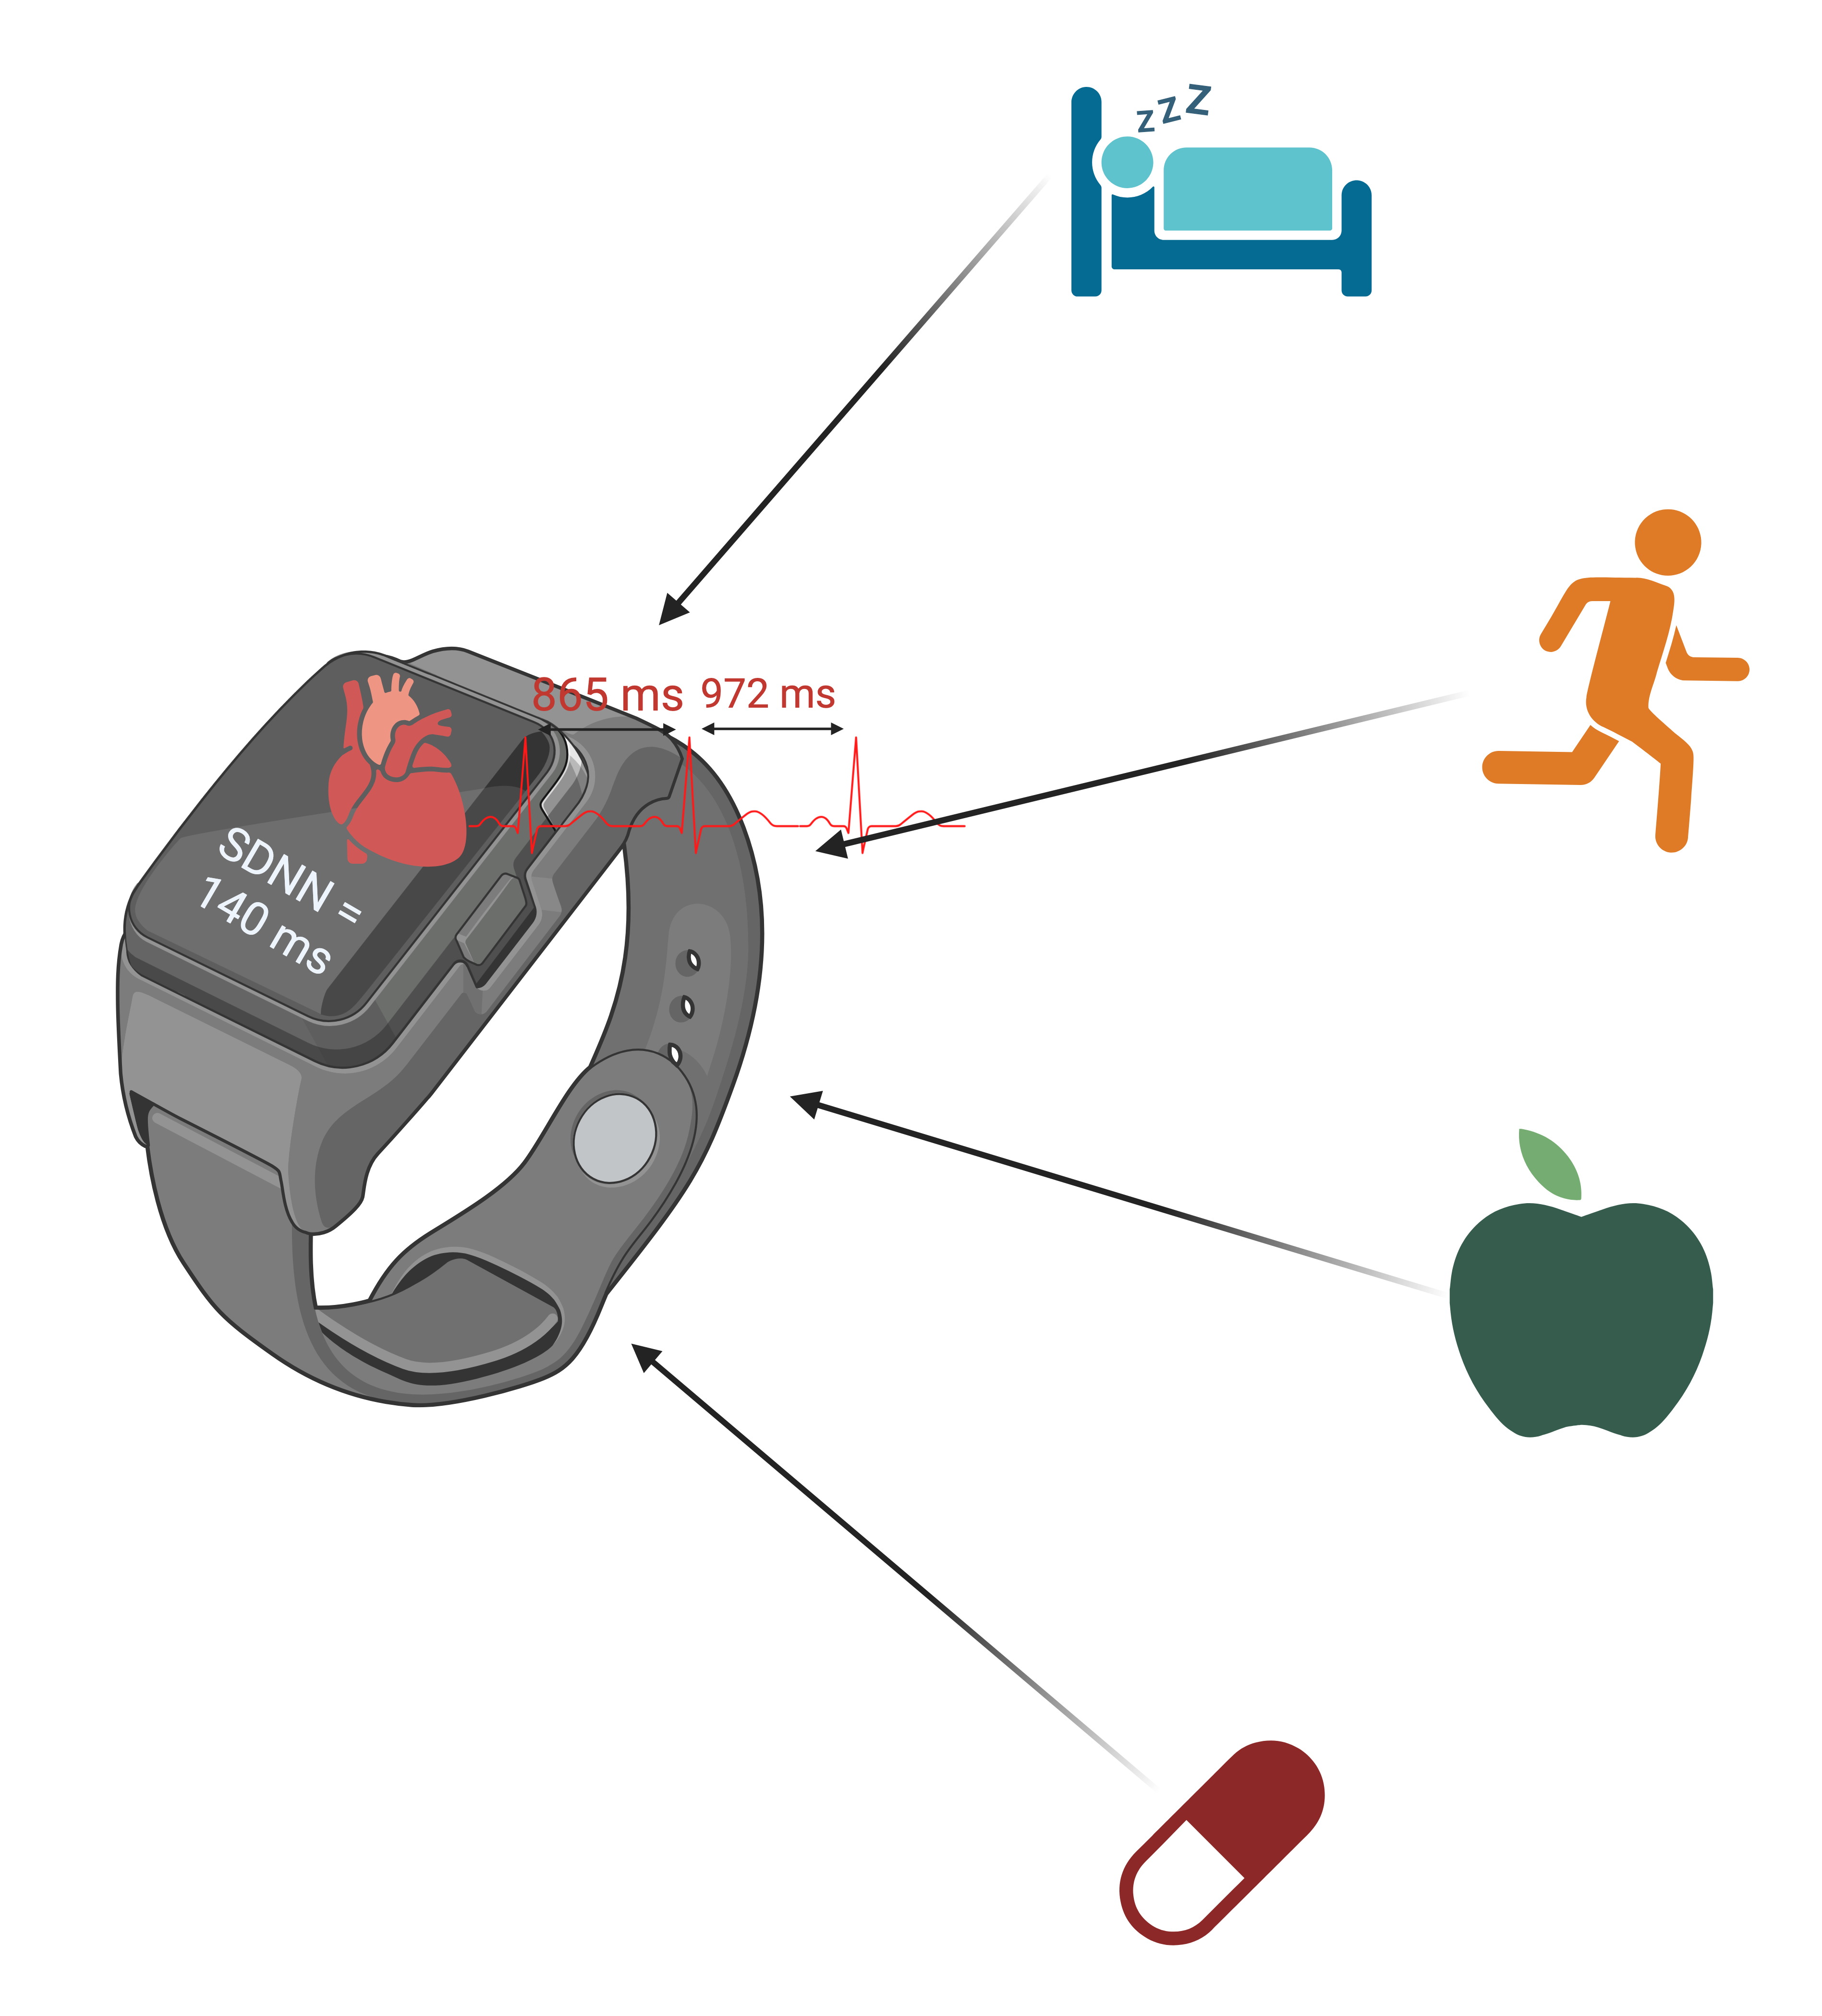
\includegraphics[width=4in,height=\textheight]{images/smartwatch.png}

}

\caption{HRV feedback in response to lifestyle and treatment
interventions. (Source: Author)}

}

\end{minipage}%

\end{figure}

Future studies can leverage wearable devices to better understand the
behavioral factors and treatment options that contribute to its
improvement or deterioration of HRV. This approach may help identify
effective lifestyle patterns or medications that improve success of
cardiovascular health through modulation of HRV.

Standardization and transparency across different brands of wearable
devices remain a challenge for both research and clinical implementation
of heart rate and HRV monitoring. While smartwatches offer a convenient
method for heart rate measurement, their accuracy can vary, as they rely
on photoplethysmography to detect pulse rate at the wrist. This method
can be imprecise under certain conditions, particularly during physical
activity, due to motion artifacts and other external
factors{[}\textsuperscript{113}{]}\textsuperscript{114}. Despite these
limitations, ongoing improvements in sensor technology and algorithm
calibration are likely to enhance the reliability of wearable-derived
heart rate and HRV data.

\hypertarget{risk-stratification-1}{%
\section{Risk-stratification}\label{risk-stratification-1}}

Based on the clinical implications, the distinct roles of long-term HRV
and CART in risk stratification remain to be demonstrated and require
further investigation.

From the perspective of wearable devices, it remains to be determined
whether HRV can serve as an early indicator of CVD risk when used in a
risk score alongside simple non-invasive markers such as age, sex, and
BMI, and how it compares to current CVD risk scores that include
blood-based biomarkers and blood pressure.

A limitation of long-term HRV measurement is the lack of
standardization, as data are collected under free-living conditions and
may be influenced by daily behaviors, potentially affecting risk
classification. Therefore, standardized procedures may be necessary.
CART has been shown to be a reliable, non-invasive method that typically
takes approximately 10 minutes to complete. As such, a standardized and
validated diagnosis of CAN can help identify patients with type 2
diabetes who are at higher risk of CVD, nephropathy, and heart failure.
However, the extent to which the diagnosis of CAN identifies heart
failure risk and is generalizable to broader populations with type 2
diabetes or even prediabetes, in a clinically relevant context, remains
to be assessed.

Our findings suggest that long-term HRV and CAN may serve as potential
markers for CVD and heart failure risk among individuals at elevated
metabolic risk, helping to identify those who could benefit from
preventive strategies. Future research should evaluate whether
individuals classified as high-risk based on autonomic dysfunction or
CAN should initiate cardiovascular-focused prevention or screening
earlier, or receive specific interventions tailored to their condition.

\begin{figure}

\begin{minipage}[t]{\linewidth}

{\centering 

\raisebox{-\height}{

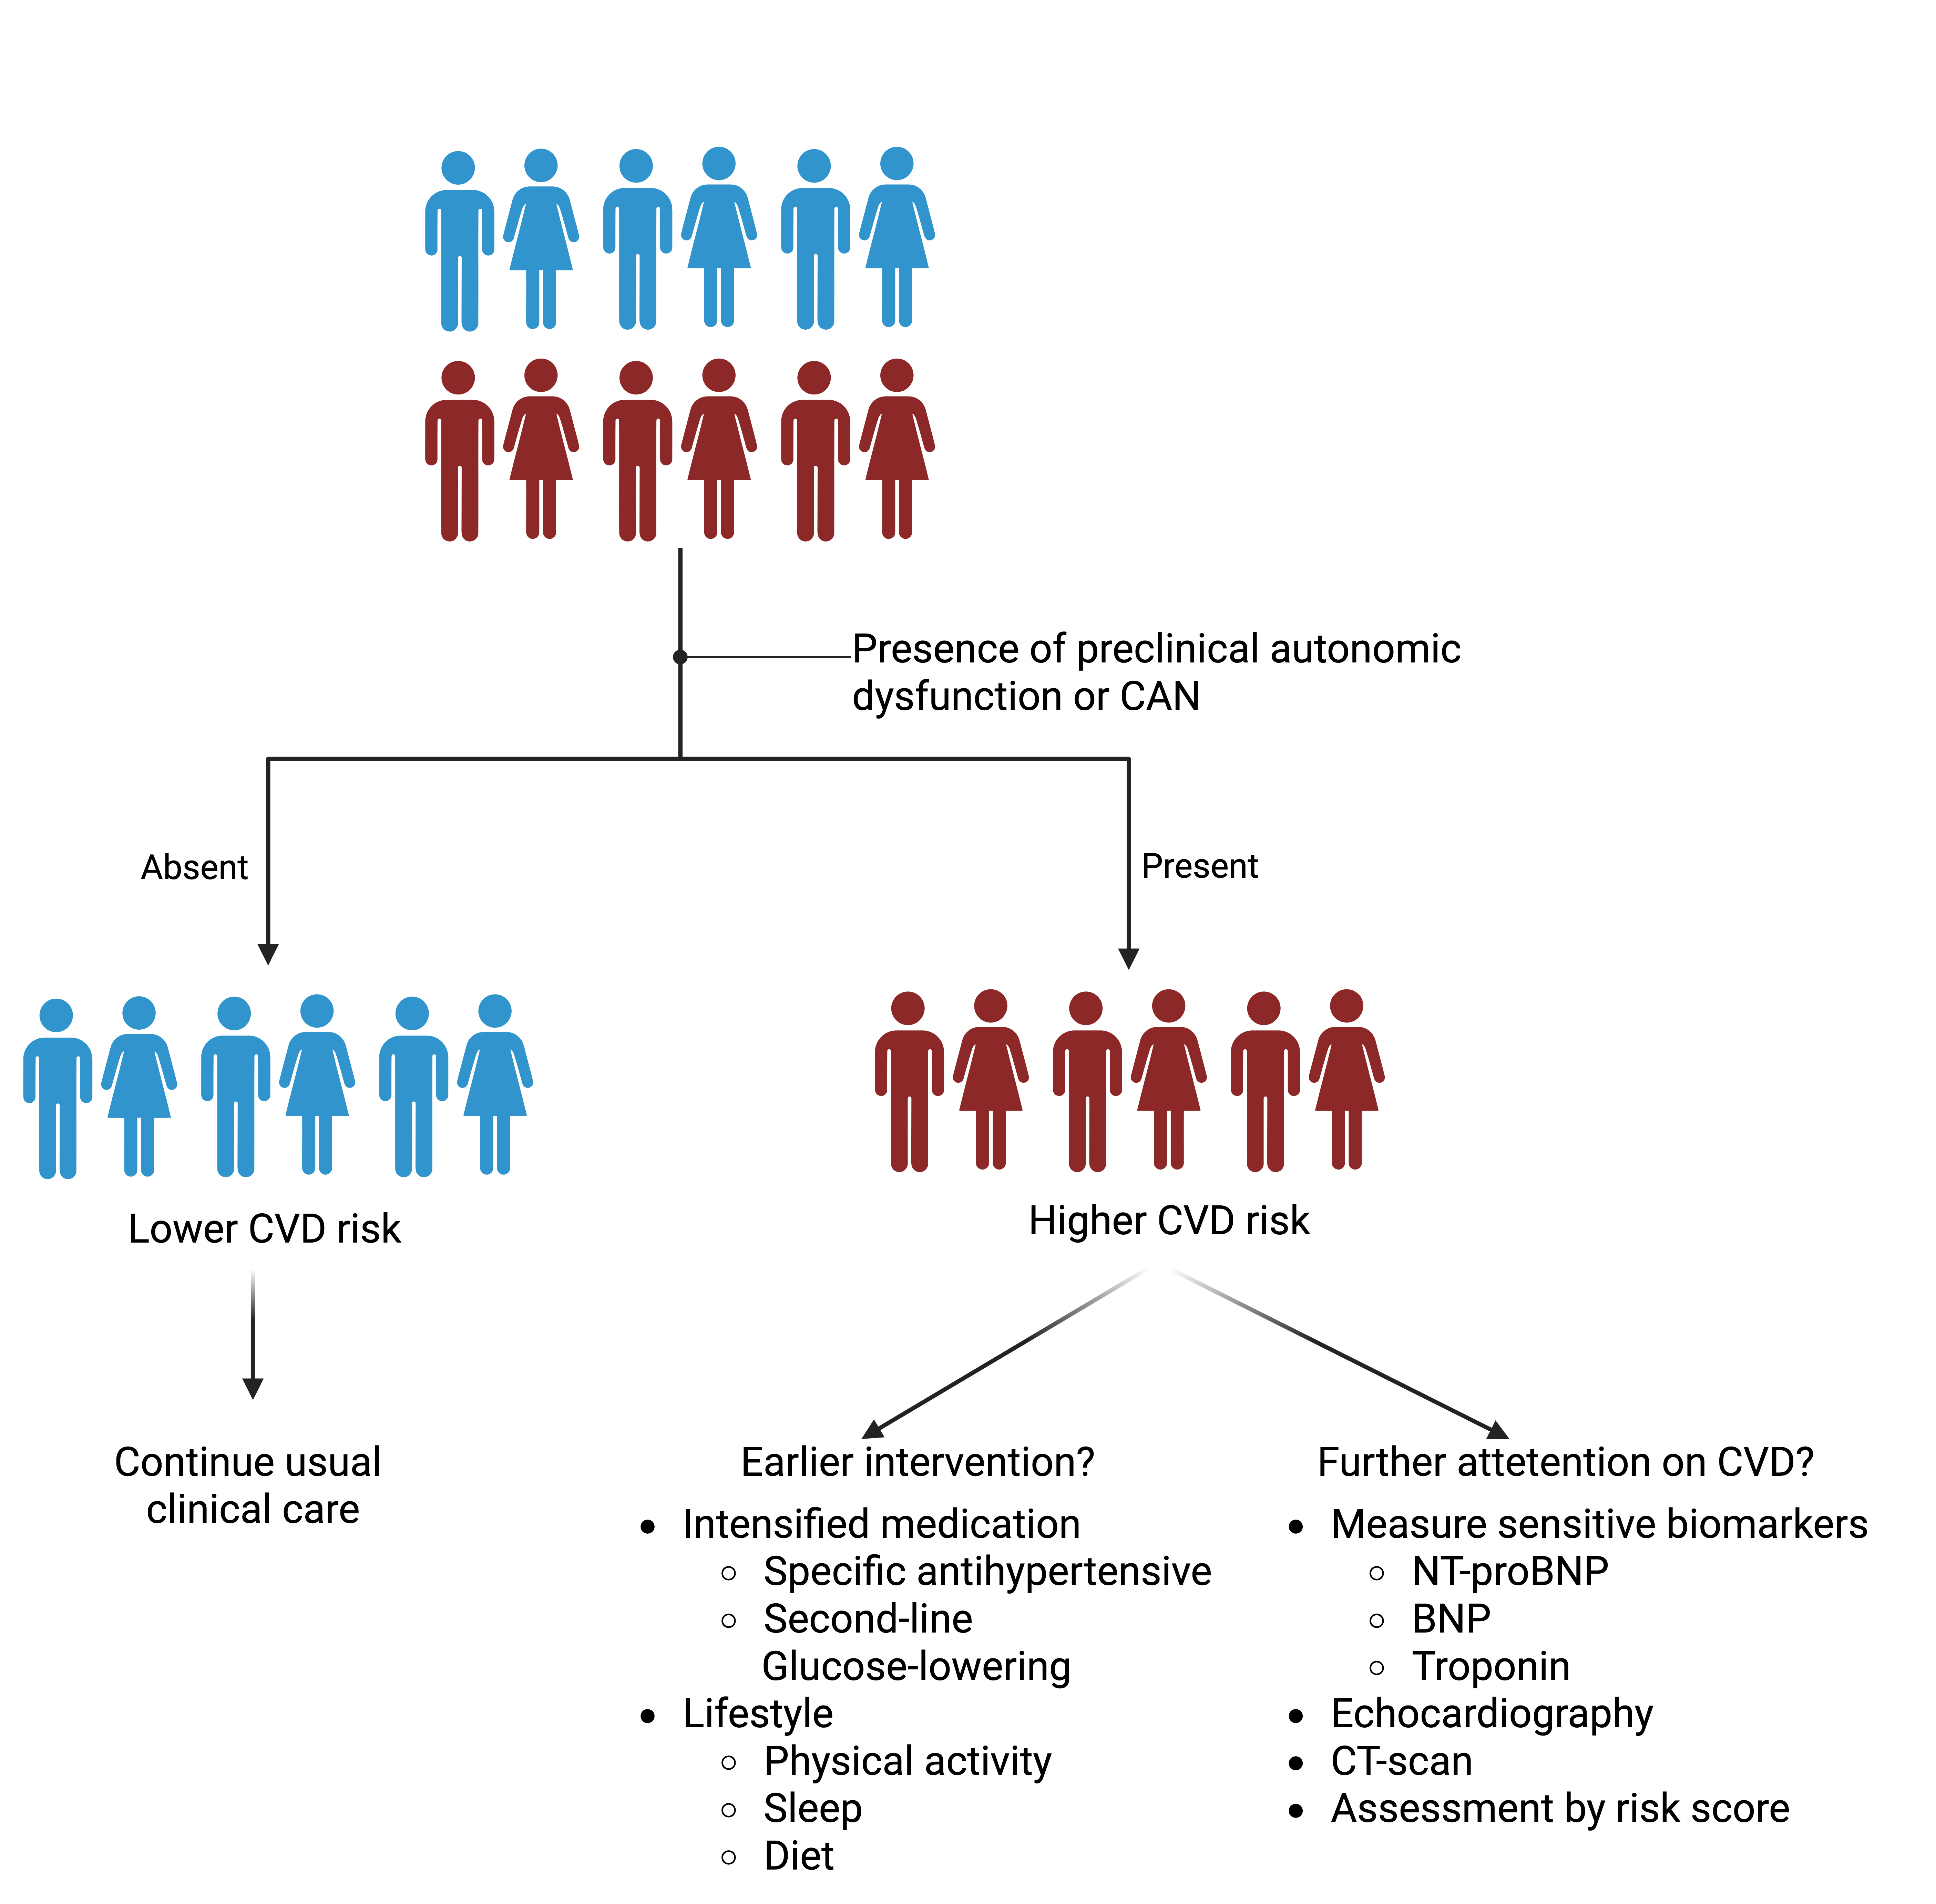
\includegraphics[width=5in,height=\textheight]{images/strafication_tree_of_CAN(1).png}

}

\caption{Risk-stratification by autonomic dysfunction. (Source: Author)}

}

\end{minipage}%

\end{figure}

\hypertarget{effective-causal-modifiable-marker}{%
\section{Effective causal modifiable
marker}\label{effective-causal-modifiable-marker}}

Our findings support an etiological link between long-term HRV and the
risk of CVD, providing initial evidence of a potential causal
relationship. However, the observed association does not confirm
causation, and further research is necessary to determine whether the
relationship between HRV and CVD risk is truly causal. Traditionally,
epidemiological research has relied on randomized controlled trials to
establish causality. However, conducting such trials to isolate the
direct effect of HRV is particularly challenging. Interventions that
influence HRV often do so indirectly, through changes in lifestyle
factors such as weight loss, inflammation, and insulin sensitivity.
Similarly, pharmacological treatments may improve HRV as a secondary
effect, for example through blood pressure reduction from
antihypertensive medications. As a result, isolating the direct
modification of HRV is difficult. To address the limitations of clinical
trials, modern epidemiological approaches such as Mendelian
randomization\textsuperscript{115} and structured causal mediation
analysis offer alternatives for inferring causality from observational
genetic studies and for estimating indirect effects using trial
data\textsuperscript{116}. To date, no GWAS has been conducted to
investigate the genetic determinants of long-term HRV. Establishing such
genetic associations is essential for understanding its genetic
architecture and for providing unconfounded estimates by using genetic
variants as proxies to assess the causal role of HRV in CVD.

\begin{figure}

\begin{minipage}[t]{\linewidth}

{\centering 

\raisebox{-\height}{

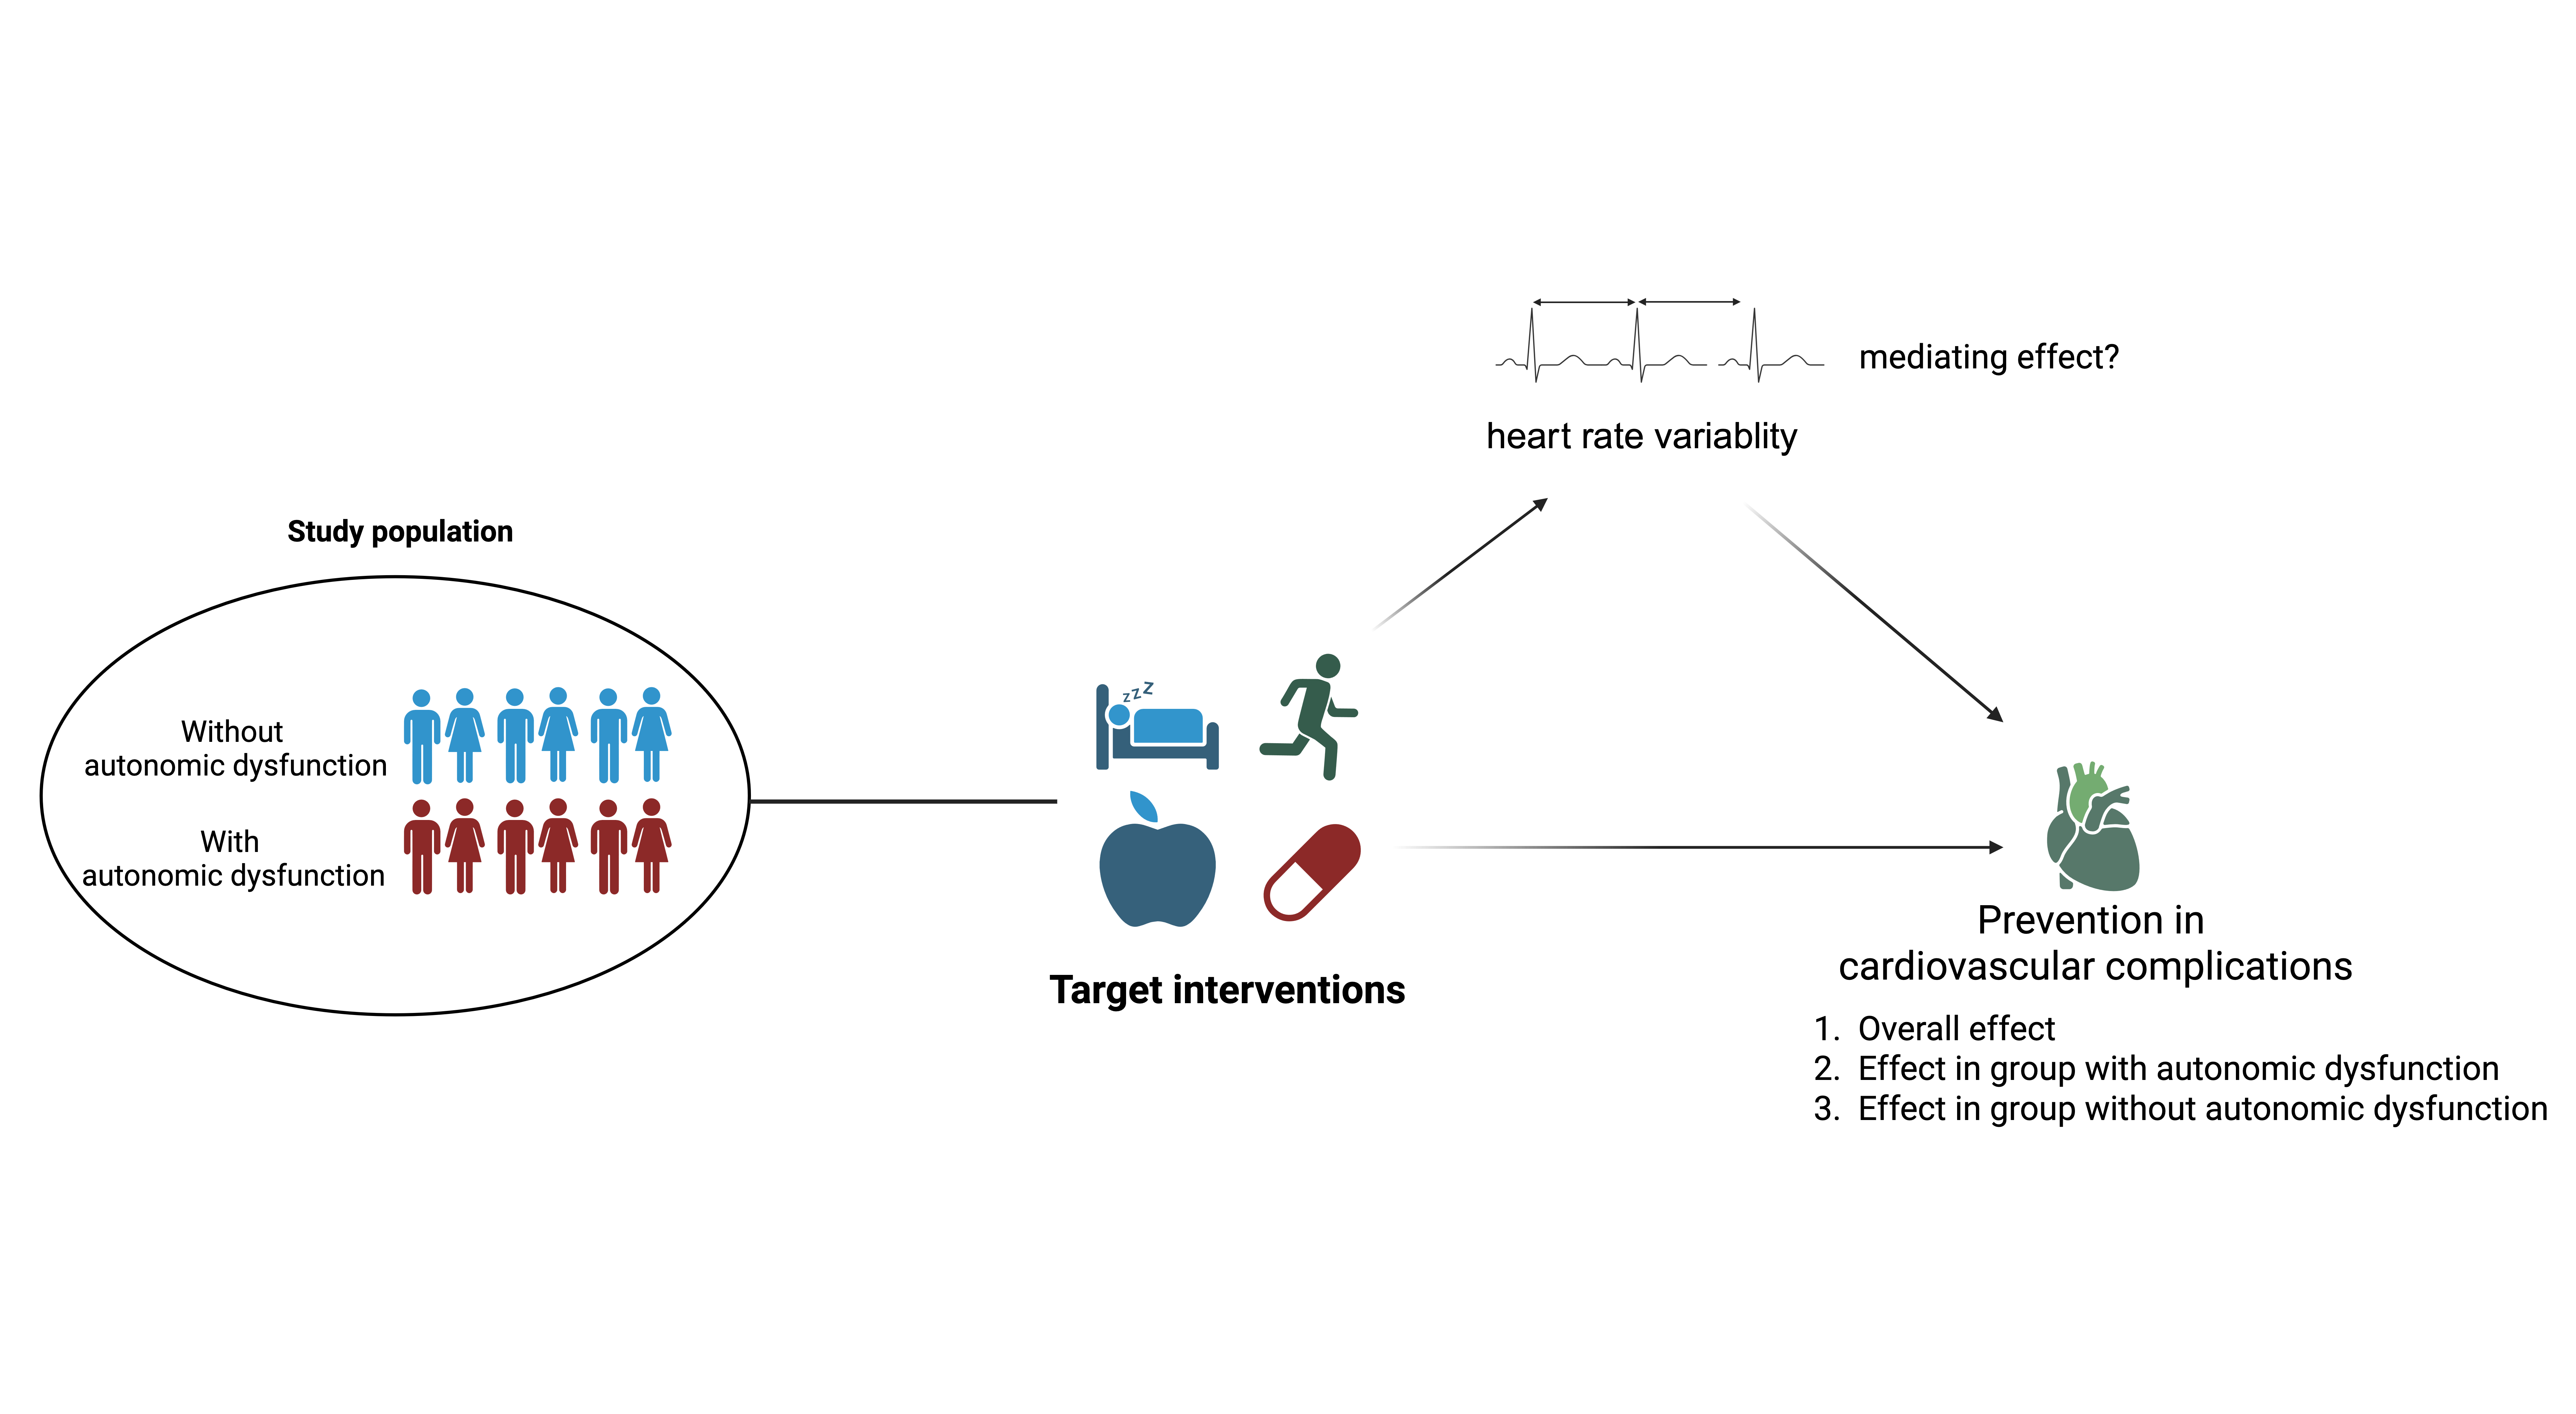
\includegraphics[width=6in,height=\textheight]{images/Mediation_HRV.png}

}

\caption{Mediation of HRV by intervention in prevention of CVD. (Source:
Author)}

}

\end{minipage}%

\end{figure}

Future cardiometabolic intervention trials, whether focused on lifestyle
modification or pharmacological treatment, should, where feasible,
include HRV measurements to enable structured mediation analyses and to
better understand whether modifying autonomic function improves
cardiovascular outcomes. This could help demonstrate whether
modification of HRV through potential strategies such as medications e.g
anti-hypertensives or lifestyle interventions including physical
activity, diet, and sleep has a sustainable effect on CVD outcomes.

\bookmarksetup{startatroot}

\hypertarget{references}{%
\chapter*{References}\label{references}}
\addcontentsline{toc}{chapter}{References}

\markboth{References}{References}

\hypertarget{refs}{}
\begin{CSLReferences}{0}{0}
\leavevmode\vadjust pre{\hypertarget{ref-diabetes2025}{}}%
\CSLLeftMargin{1 }%
\CSLRightInline{International Diabetes Federation. Diabetes atlas, 11th
Edition. International Diabetes Federation, 2025.}

\leavevmode\vadjust pre{\hypertarget{ref-magliano2022}{}}%
\CSLLeftMargin{2 }%
\CSLRightInline{Magliano DJ, Chen L, Carstensen B, \emph{et al.}
\href{https://doi.org/10.1016/S2213-8587(21)00327-2}{Trends in all-cause
mortality among people with diagnosed diabetes in high-income settings:
A multicountry analysis of aggregate data}. \emph{The Lancet Diabetes \&
Endocrinology} 2022; \textbf{10}: 112--9.}

\leavevmode\vadjust pre{\hypertarget{ref-zamana}{}}%
\CSLLeftMargin{3 }%
\CSLRightInline{Zaman S, Wasfy JH, Kapil V, \emph{et al.} The lancet
commission on rethinking coronary artery disease: Moving from ischaemia
to atheroma. \emph{The Lancet}
DOI:\href{https://doi.org/10.1016/S0140-6736(25)00055-8}{10.1016/S0140-6736(25)00055-8}.}

\leavevmode\vadjust pre{\hypertarget{ref-pop-busui2022}{}}%
\CSLLeftMargin{4 }%
\CSLRightInline{Pop-Busui R, Januzzi JL, Bruemmer D, \emph{et al.}
\href{https://doi.org/10.2337/dci22-0014}{Heart failure: An
underappreciated complication of diabetes. A consensus report of the
american diabetes association}. \emph{Diabetes Care} 2022; \textbf{45}:
1670--90.}

\leavevmode\vadjust pre{\hypertarget{ref-hillebrand2013}{}}%
\CSLLeftMargin{5 }%
\CSLRightInline{Hillebrand S, Gast KB, Mutsert R de, \emph{et al.}
\href{https://doi.org/10.1093/europace/eus341}{Heart rate variability
and first cardiovascular event in populations without known
cardiovascular disease: Meta-analysis and dose{\textendash}response
meta-regression}. \emph{EP Europace} 2013; \textbf{15}: 742--9.}

\leavevmode\vadjust pre{\hypertarget{ref-taskforceoftheeuropeansocietyofcardiologythenorthamericansocietyofpacingelectrophysiology1996}{}}%
\CSLLeftMargin{6 }%
\CSLRightInline{Task Force of the European Society of Cardiology the
North American Society of Pacing Electrophysiology.
\href{https://doi.org/doi:10.1161/01.CIR.93.5.1043}{Heart rate
variability}. \emph{Circulation} 1996; \textbf{93}: 1043--65.}

\leavevmode\vadjust pre{\hypertarget{ref-eleftheriadou2024}{}}%
\CSLLeftMargin{7 }%
\CSLRightInline{Eleftheriadou A, Spallone V, Tahrani AA, Alam U.
\href{https://doi.org/10.1007/s00125-024-06242-0}{Cardiovascular
autonomic neuropathy in diabetes: An update with a focus on management}.
\emph{Diabetologia} 2024; \textbf{67}: 2611--25.}

\leavevmode\vadjust pre{\hypertarget{ref-coopmans2020}{}}%
\CSLLeftMargin{8 }%
\CSLRightInline{Coopmans C, Zhou TL, Henry RMA, \emph{et al.}
\href{https://doi.org/10.2337/dc19-2367}{Both prediabetes and type 2
diabetes are associated with lower heart rate variability: The
maastricht study}. \emph{Diabetes Care} 2020; \textbf{43}: 1126--33.}

\leavevmode\vadjust pre{\hypertarget{ref-rooney2023}{}}%
\CSLLeftMargin{9 }%
\CSLRightInline{Rooney MR, Fang M, Ogurtsova K, \emph{et al.}
\href{https://doi.org/10.2337/dc22-2376}{Global prevalence of
prediabetes}. \emph{Diabetes Care} 2023; \textbf{46}: 1388--94.}

\leavevmode\vadjust pre{\hypertarget{ref-birkenfeld2024}{}}%
\CSLLeftMargin{10 }%
\CSLRightInline{Birkenfeld AL, Franks PW, Mohan V.
\href{https://doi.org/10.1161/CIRCULATIONAHA.124.070463}{Precision
medicine in people at risk for diabetes and atherosclerotic
cardiovascular disease: A fresh perspective on prevention}.
\emph{Circulation} 2024; \textbf{150}: 1910--2.}

\leavevmode\vadjust pre{\hypertarget{ref-dhingra2023}{}}%
\CSLLeftMargin{11 }%
\CSLRightInline{Dhingra LS, Aminorroaya A, Oikonomou EK, \emph{et al.}
\href{https://doi.org/10.1001/jamanetworkopen.2023.16634}{Use of
wearable devices in individuals with or at risk for cardiovascular
disease in the US, 2019 to 2020}. \emph{JAMA Network Open} 2023;
\textbf{6}: e2316634--4.}

\leavevmode\vadjust pre{\hypertarget{ref-bayoumy2021}{}}%
\CSLLeftMargin{12 }%
\CSLRightInline{Bayoumy K, Gaber M, Elshafeey A, \emph{et al.}
\href{https://doi.org/10.1038/s41569-021-00522-7}{Smart wearable devices
in cardiovascular care: Where we are and how to move forward}.
\emph{Nature Reviews Cardiology} 2021; \textbf{18}: 581--99.}

\leavevmode\vadjust pre{\hypertarget{ref-natarajan2020}{}}%
\CSLLeftMargin{13 }%
\CSLRightInline{Natarajan A, Pantelopoulos A, Emir-Farinas H, Natarajan
P. \href{https://doi.org/10.1016/S2589-7500(20)30246-6}{Heart rate
variability with photoplethysmography in 8 million individuals: A
cross-sectional study}. \emph{The Lancet Digital Health} 2020;
\textbf{2}: e650--7.}

\leavevmode\vadjust pre{\hypertarget{ref-tabuxe1k2012}{}}%
\CSLLeftMargin{14 }%
\CSLRightInline{Tabák AG, Herder C, Rathmann W, Brunner EJ, Kivimäki M.
\href{https://doi.org/10.1016/S0140-6736(12)60283-9}{Prediabetes: A
high-risk state for diabetes development}. \emph{The Lancet} 2012;
\textbf{379}: 2279--90.}

\leavevmode\vadjust pre{\hypertarget{ref-bonora2018}{}}%
\CSLLeftMargin{15 }%
\CSLRightInline{Bonora E, DeFronzo R. Diabetes. Epidemiology, genetics,
pathogenesis, diagnosis, prevention, and treatment. 2018
DOI:\href{https://doi.org/10.1007/978-3-319-27317-4}{10.1007/978-3-319-27317-4}.}

\leavevmode\vadjust pre{\hypertarget{ref-worldhealthorganization2020}{}}%
\CSLLeftMargin{16 }%
\CSLRightInline{World Health Organization. Diagnosis and management of
type 2 diabetes (HEARTS-d). Geneva, 2020.}

\leavevmode\vadjust pre{\hypertarget{ref-americandiabetesassociationprofessionalpracticecommittee2021}{}}%
\CSLLeftMargin{17 }%
\CSLRightInline{American Diabetes Association Professional Practice
Committee. \href{https://doi.org/10.2337/dc22-S002}{2. Classification
and diagnosis of diabetes: Standards of medical care in
diabetes{\textemdash}2022}. \emph{Diabetes Care} 2021; \textbf{45}:
S17--38.}

\leavevmode\vadjust pre{\hypertarget{ref-mokhtar2023}{}}%
\CSLLeftMargin{18 }%
\CSLRightInline{Mokhtar SBA, Heide FCT van der, Oyaert KAM, \emph{et
al.} \href{https://doi.org/10.1007/s00125-023-05986-5}{(Pre)diabetes and
a higher level of glycaemic measures are continuously associated with
corneal neurodegeneration assessed by corneal confocal microscopy: The
maastricht study}. \emph{Diabetologia} 2023; \textbf{66}: 2030--41.}

\leavevmode\vadjust pre{\hypertarget{ref-huang2014}{}}%
\CSLLeftMargin{19 }%
\CSLRightInline{Huang Y, Cai X, Qiu M, \emph{et al.}
\href{https://doi.org/10.1007/s00125-014-3361-2}{Prediabetes and the
risk of cancer: A meta-analysis}. \emph{Diabetologia} 2014; \textbf{57}:
2261--9.}

\leavevmode\vadjust pre{\hypertarget{ref-stehouwer2018}{}}%
\CSLLeftMargin{20 }%
\CSLRightInline{Stehouwer CDA.
\href{https://doi.org/10.2337/dbi17-0044}{Microvascular dysfunction and
hyperglycemia: A vicious cycle with widespread consequences}.
\emph{Diabetes} 2018; \textbf{67}: 1729--41.}

\leavevmode\vadjust pre{\hypertarget{ref-taylor2013}{}}%
\CSLLeftMargin{21 }%
\CSLRightInline{Taylor R. \href{https://doi.org/10.2337/dc12-1805}{Type
2 diabetes: Etiology and reversibility}. \emph{Diabetes Care} 2013;
\textbf{36}: 1047--55.}

\leavevmode\vadjust pre{\hypertarget{ref-fuxe6rch2013}{}}%
\CSLLeftMargin{22 }%
\CSLRightInline{Færch K, Witte DR, Tabák AG, \emph{et al.}
\href{https://doi.org/10.1016/S2213-8587(13)70008-1}{Trajectories of
cardiometabolic risk factors before diagnosis of three subtypes of type
2 diabetes: a post-hoc analysis of the longitudinal Whitehall II cohort
study.} \emph{The lancet Diabetes \& endocrinology} 2013; \textbf{1}:
43--51.}

\leavevmode\vadjust pre{\hypertarget{ref-ritchie2020}{}}%
\CSLLeftMargin{23 }%
\CSLRightInline{Ritchie RH, Abel ED.
\href{https://doi.org/10.1161/CIRCRESAHA.120.315913}{Basic mechanisms of
diabetic heart disease}. \emph{Circulation Research} 2020; \textbf{126}:
1501--25.}

\leavevmode\vadjust pre{\hypertarget{ref-yusuf2020}{}}%
\CSLLeftMargin{24 }%
\CSLRightInline{Yusuf S, Joseph P, Rangarajan S, \emph{et al.}
\href{https://doi.org/10.1016/S0140-6736(19)32008-2}{Modifiable risk
factors, cardiovascular disease, and mortality in 155{\hphantom{,}}722
individuals from 21 high-income, middle-income, and low-income countries
(PURE): A prospective cohort study}. \emph{The Lancet} 2020;
\textbf{395}: 795--808.}

\leavevmode\vadjust pre{\hypertarget{ref-mitchell2020}{}}%
\CSLLeftMargin{25 }%
\CSLRightInline{Mitchell GF, Powell JT.
\href{https://doi.org/10.1161/ATVBAHA.120.314208}{Arteriosclerosis}.
\emph{Arteriosclerosis, Thrombosis, and Vascular Biology} 2020;
\textbf{40}: 1025--7.}

\leavevmode\vadjust pre{\hypertarget{ref-lee2010}{}}%
\CSLLeftMargin{26 }%
\CSLRightInline{Lee H-Y, Oh B-H.
\href{https://doi.org/10.1253/circj.CJ-10-0910}{Aging and arterial
stiffness}. \emph{Circulation Journal} 2010; \textbf{74}: 2257--62.}

\leavevmode\vadjust pre{\hypertarget{ref-lu2023}{}}%
\CSLLeftMargin{27 }%
\CSLRightInline{Lu Y, Kiechl SJ, Wang J, Xu Q, Kiechl S, Pechlaner R.
\href{https://doi.org/10.1016/j.ebiom.2023.104619}{Global distributions
of age- and sex-related arterial stiffness: systematic review and
meta-analysis of 167 studies with 509,743 participants}.
\emph{EBioMedicine} 2023; \textbf{92}: 104619.}

\leavevmode\vadjust pre{\hypertarget{ref-zhong2018}{}}%
\CSLLeftMargin{28 }%
\CSLRightInline{Zhong Q, Hu M-J, Cui Y-J, \emph{et al.}
\href{https://doi.org/10.1177/0003319717742544}{Carotid{\textendash}femoral
pulse wave velocity in the prediction of cardiovascular events and
mortality: An updated systematic review and meta-analysis}.
\emph{Angiology} 2018; \textbf{69}: 617--29.}

\leavevmode\vadjust pre{\hypertarget{ref-kawai2024}{}}%
\CSLLeftMargin{29 }%
\CSLRightInline{Kawai K, Kawakami R, Finn AV, Virmani R.
\href{https://doi.org/10.1161/ATVBAHA.124.319396}{Differences in stable
and unstable atherosclerotic plaque}. \emph{Arteriosclerosis,
Thrombosis, and Vascular Biology} 2024; \textbf{44}: 1474--84.}

\leavevmode\vadjust pre{\hypertarget{ref-alasady2013}{}}%
\CSLLeftMargin{30 }%
\CSLRightInline{Alasady M, Shipp NJ, Brooks AG, \emph{et al.}
\href{https://doi.org/10.1161/CIRCEP.113.000163}{Myocardial infarction
and atrial fibrillation}. \emph{Circulation: Arrhythmia and
Electrophysiology} 2013; \textbf{6}: 738--45.}

\leavevmode\vadjust pre{\hypertarget{ref-elgendy2019}{}}%
\CSLLeftMargin{31 }%
\CSLRightInline{Elgendy IY, Mahtta D, Pepine CJ.
\href{https://doi.org/10.1161/CIRCRESAHA.118.313568}{Medical therapy for
heart failure caused by ischemic heart disease}. \emph{Circulation
Research} 2019; \textbf{124}: 1520--35.}

\leavevmode\vadjust pre{\hypertarget{ref-bilano2015}{}}%
\CSLLeftMargin{32 }%
\CSLRightInline{Bilano V, Gilmour S, Moffiet T, \emph{et al.}
\href{https://doi.org/10.1016/S0140-6736(15)60264-1}{Global trends and
projections for tobacco use, 1990{\textendash}2025: An analysis of
smoking indicators from the WHO comprehensive information systems for
tobacco control}. \emph{The Lancet} 2015; \textbf{385}: 966--76.}

\leavevmode\vadjust pre{\hypertarget{ref-ockene1997}{}}%
\CSLLeftMargin{33 }%
\CSLRightInline{Ockene IS, Miller NH.
\href{https://doi.org/10.1161/01.CIR.96.9.3243}{Cigarette smoking,
cardiovascular disease, and stroke}. \emph{Circulation} 1997;
\textbf{96}: 3243--7.}

\leavevmode\vadjust pre{\hypertarget{ref-shah2015}{}}%
\CSLLeftMargin{34 }%
\CSLRightInline{Shah AD, Langenberg C, Rapsomaniki E, \emph{et al.}
\href{https://doi.org/10.1016/S2213-8587(14)70219-0}{Type 2 diabetes and
incidence of cardiovascular diseases: A cohort study in 1·9 million
people}. \emph{The Lancet Diabetes \& Endocrinology} 2015; \textbf{3}:
105--13.}

\leavevmode\vadjust pre{\hypertarget{ref-donnan2008}{}}%
\CSLLeftMargin{35 }%
\CSLRightInline{Donnan GA, Fisher M, Macleod M, Davis SM.
\href{https://doi.org/10.1016/S0140-6736(08)60694-7}{Stroke}. \emph{The
Lancet} 2008; \textbf{371}: 1612--23.}

\leavevmode\vadjust pre{\hypertarget{ref-vos2020}{}}%
\CSLLeftMargin{36 }%
\CSLRightInline{Vos T, Lim SS, Abbafati C, \emph{et al.}
\href{https://doi.org/10.1016/S0140-6736(20)30925-9}{Global burden of
369 diseases and injuries in 204 countries and territories,
1990{\textendash}2019: A systematic analysis for the global burden of
disease study 2019}. \emph{The Lancet} 2020; \textbf{396}: 1204--22.}

\leavevmode\vadjust pre{\hypertarget{ref-li2024}{}}%
\CSLLeftMargin{37 }%
\CSLRightInline{Li X, Kong X, Yang C, \emph{et al.} Global, regional,
and national burden of ischemic stroke, 1990{\textendash}2021: An
analysis of data from the global burden of disease study 2021.
\emph{eClinicalMedicine} 2024; \textbf{75}.
DOI:\href{https://doi.org/10.1016/j.eclinm.2024.102758}{10.1016/j.eclinm.2024.102758}.}

\leavevmode\vadjust pre{\hypertarget{ref-lee2012}{}}%
\CSLLeftMargin{38 }%
\CSLRightInline{Lee M, Saver JL, Hong K-S, Song S, Chang K-H, Ovbiagele
B. \href{https://doi.org/10.1136/bmj.e3564}{Effect of pre-diabetes on
future risk of stroke: Meta-analysis}. \emph{BMJ : British Medical
Journal} 2012; \textbf{344}: e3564.}

\leavevmode\vadjust pre{\hypertarget{ref-barr2007}{}}%
\CSLLeftMargin{39 }%
\CSLRightInline{Barr ELM, Zimmet PZ, Welborn TA, \emph{et al.}
\href{https://doi.org/10.1161/CIRCULATIONAHA.106.685628}{Risk of
cardiovascular and all-cause mortality in individuals with diabetes
mellitus, impaired fasting glucose, and impaired glucose tolerance}.
\emph{Circulation} 2007; \textbf{116}: 151--7.}

\leavevmode\vadjust pre{\hypertarget{ref-khan2024}{}}%
\CSLLeftMargin{40 }%
\CSLRightInline{Khan MS, Shahid I, Bennis A, Rakisheva A, Metra M,
Butler J. \href{https://doi.org/10.1038/s41569-024-01046-6}{Global
epidemiology of heart failure}. \emph{Nature Reviews Cardiology} 2024;
\textbf{21}: 717--34.}

\leavevmode\vadjust pre{\hypertarget{ref-normand2019}{}}%
\CSLLeftMargin{41 }%
\CSLRightInline{Normand C, Kaye DM, Povsic TJ, Dickstein K.
\href{https://doi.org/10.1016/S0140-6736(18)32216-5}{Beyond
pharmacological treatment: An insight into therapies that target
specific aspects of heart failure pathophysiology}. \emph{The Lancet}
2019; \textbf{393}: 1045--55.}

\leavevmode\vadjust pre{\hypertarget{ref-campbell2024}{}}%
\CSLLeftMargin{42 }%
\CSLRightInline{Campbell P, Rutten FH, Lee MM, Hawkins NM, Petrie MC.
\href{https://doi.org/10.1016/S0140-6736(23)02756-3}{Heart failure with
preserved ejection fraction: everything the clinician needs to know.}
\emph{Lancet (London, England)} 2024; \textbf{403}: 1083--92.}

\leavevmode\vadjust pre{\hypertarget{ref-schlaich2015}{}}%
\CSLLeftMargin{43 }%
\CSLRightInline{Schlaich M, Straznicky N, Lambert E, Lambert G.
\href{https://doi.org/10.1016/s2213-8587(14)70033-6}{Metabolic syndrome:
a sympathetic disease?} \emph{Lancet Diabetes Endocrinol} 2015;
\textbf{3}: 148--57.}

\leavevmode\vadjust pre{\hypertarget{ref-rinaldi2023}{}}%
\CSLLeftMargin{44 }%
\CSLRightInline{Rinaldi E, Heide FCT van der, Bonora E, \emph{et al.}
\href{https://doi.org/10.1186/s12933-023-01837-0}{Lower heart rate
variability, an index of worse autonomic function, is associated with
worse beta cell response to a glycemic load in vivo{\textemdash}the
maastricht study}. \emph{Cardiovascular Diabetology} 2023; \textbf{22}:
105.}

\leavevmode\vadjust pre{\hypertarget{ref-huggett2003}{}}%
\CSLLeftMargin{45 }%
\CSLRightInline{Huggett RJ, Scott EM, Gilbey SG, Stoker JB, Mackintosh
AF, Mary DASG.
\href{https://doi.org/10.1161/01.CIR.0000103123.66264.FE}{Impact of type
2 diabetes mellitus on sympathetic neural mechanisms in hypertension}.
\emph{Circulation} 2003; \textbf{108}: 3097--101.}

\leavevmode\vadjust pre{\hypertarget{ref-cseh2020}{}}%
\CSLLeftMargin{46 }%
\CSLRightInline{Cseh D, Climie RE, Offredo L, \emph{et al.}
\href{https://doi.org/10.1161/ATVBAHA.120.314102}{Type 2 diabetes
mellitus is independently associated with decreased neural baroreflex
sensitivity}. \emph{Arteriosclerosis, Thrombosis, and Vascular Biology}
2020; \textbf{40}: 1420--8.}

\leavevmode\vadjust pre{\hypertarget{ref-hansen2025}{}}%
\CSLLeftMargin{47 }%
\CSLRightInline{Hansen CS, Christensen MMB, Vistisen D, \emph{et al.}
\href{https://doi.org/10.1007/s10286-024-01069-6}{Normative data on
measures of cardiovascular autonomic neuropathy and the effect of
pretest conditions in a large danish non-diabetic CVD-free population
from the lolland-falster health study}. \emph{Clinical Autonomic
Research} 2025; \textbf{35}: 101--13.}

\leavevmode\vadjust pre{\hypertarget{ref-reductio2002}{}}%
\CSLLeftMargin{48 }%
\CSLRightInline{\href{https://doi.org/10.1056/NEJMoa012512}{Reduction in
the incidence of type 2 diabetes with lifestyle intervention or
metformin}. \emph{New England Journal of Medicine} 2002; \textbf{346}:
393--403.}

\leavevmode\vadjust pre{\hypertarget{ref-kahn2024}{}}%
\CSLLeftMargin{49 }%
\CSLRightInline{Kahn SE, Deanfield JE, Jeppesen OK, \emph{et al.}
\href{https://doi.org/10.2337/dc24-0491}{Effect of semaglutide on
regression and progression of glycemia in people with overweight or
obesity but without diabetes in the SELECT trial}. \emph{Diabetes Care}
2024; \textbf{47}: 1350--9.}

\leavevmode\vadjust pre{\hypertarget{ref-umetani1998}{}}%
\CSLLeftMargin{50 }%
\CSLRightInline{Umetani K, Singer DH, McCraty R, Atkinson M.
\href{https://doi.org/10.1016/S0735-1097(97)00554-8}{Twenty-four hour
time domain heart rate variability and heart rate: Relations to age and
gender over nine decades}. \emph{Journal of the American College of
Cardiology} 1998; \textbf{31}: 593--601.}

\leavevmode\vadjust pre{\hypertarget{ref-serrador1999}{}}%
\CSLLeftMargin{51 }%
\CSLRightInline{Serrador JM, Finlayson HC, Hughson RL.
\href{https://doi.org/10.1136/hrt.82.6.e9}{Physical activity is a major
contributor to the ultra low frequency components of heart rate
variability}. \emph{Heart} 1999; \textbf{82}: e9.}

\leavevmode\vadjust pre{\hypertarget{ref-akselrod1981}{}}%
\CSLLeftMargin{52 }%
\CSLRightInline{Akselrod S, Gordon D, Ubel FA, Shannon DC, Berger AC,
Cohen RJ. \href{https://doi.org/10.1126/science.6166045}{Power spectrum
analysis of heart rate fluctuation: A quantitative probe of beat-to-beat
cardiovascular control}. \emph{Science} 1981; \textbf{213}: 220--2.}

\leavevmode\vadjust pre{\hypertarget{ref-taylor1998}{}}%
\CSLLeftMargin{53 }%
\CSLRightInline{Taylor JA, Carr DL, Myers CW, Eckberg DL.
\href{https://doi.org/10.1161/01.CIR.98.6.547}{Mechanisms underlying
very-low-frequency RR-interval oscillations in humans}.
\emph{Circulation} 1998; \textbf{98}: 547--55.}

\leavevmode\vadjust pre{\hypertarget{ref-jeffreyj.goldberger2019}{}}%
\CSLLeftMargin{54 }%
\CSLRightInline{Jeffrey J. Goldberger, Rishi Arora, Una Buckley,
Kalyanam Shivkumar.
\href{https://doi.org/doi:10.1016/j.jacc.2018.12.064}{Autonomic nervous
system dysfunction}. \emph{Journal of the American College of
Cardiology} 2019; \textbf{73}: 1189--206.}

\leavevmode\vadjust pre{\hypertarget{ref-mccraty2015}{}}%
\CSLLeftMargin{55 }%
\CSLRightInline{Mccraty R, Shaffer F.
\href{https://doi.org/10.7453/gahmj.2014.073}{Heart rate variability:
New perspectives on physiological mechanisms, assessment of
self-regulatory capacity, and health risk}. \emph{Global Advances in
Health and Medicine} 2015; \textbf{4}: 46--61.}

\leavevmode\vadjust pre{\hypertarget{ref-elghozi1991}{}}%
\CSLLeftMargin{56 }%
\CSLRightInline{Elghozi J-L, Laude D, Girard A.
\href{https://doi.org/10.1111/j.1440-1681.1991.tb01391.x}{EFFECTS OF
RESPIRATION ON BLOOD PRESSURE AND HEART RATE VARIABILITY IN HUMANS}.
\emph{Clinical and Experimental Pharmacology and Physiology} 1991;
\textbf{18}: 735--42.}

\leavevmode\vadjust pre{\hypertarget{ref-schaarup2024a}{}}%
\CSLLeftMargin{57 }%
\CSLRightInline{Schaarup J. Actiheart validation of time-domain heart
rate variability. 2024.
\url{https://figshare.com/articles/online_resource/Actiheart_validation_of_time-domain_heart_rate_variability/26182361}.}

\leavevmode\vadjust pre{\hypertarget{ref-tanlaizhou2018}{}}%
\CSLLeftMargin{58 }%
\CSLRightInline{Tan Lai Zhou, Ronald M. A. Henry, Coen D. A. Stehouwer,
Thomas T. van Sloten, Koen D. Reesink, Abraham A. Kroon.
\href{https://doi.org/doi:10.1161/HYPERTENSIONAHA.118.11325}{Blood
pressure variability, arterial stiffness, and arterial remodeling}.
\emph{Hypertension} 2018; \textbf{72}: 1002--10.}

\leavevmode\vadjust pre{\hypertarget{ref-whoneed2012}{}}%
\CSLLeftMargin{59 }%
\CSLRightInline{Bendix Carstensen Steno Diabetes Center. Who needs the
cox model anyway. \emph{Stat Med} 2012; \textbf{31}: 10741088.}

\leavevmode\vadjust pre{\hypertarget{ref-knol2012}{}}%
\CSLLeftMargin{60 }%
\CSLRightInline{Knol MJ, VanderWeele TJ.
\href{https://doi.org/10.1093/ije/dyr218}{Recommendations for presenting
analyses of effect modification and interaction}. \emph{International
Journal of Epidemiology} 2012; \textbf{41}: 514--20.}

\leavevmode\vadjust pre{\hypertarget{ref-hughes2019}{}}%
\CSLLeftMargin{61 }%
\CSLRightInline{Hughes RA, Heron J, Sterne JAC, Tilling K.
\href{https://doi.org/10.1093/ije/dyz032}{Accounting for missing data in
statistical analyses: Multiple imputation is not always the answer}.
\emph{International Journal of Epidemiology} 2019; \textbf{48}:
1294--304.}

\leavevmode\vadjust pre{\hypertarget{ref-angelaberos2023}{}}%
\CSLLeftMargin{62 }%
\CSLRightInline{Angela Beros, John Sluyter, Robert Keith Rhodes Scragg.
\href{https://doi.org/10.1136/bmjdrc-2022-003140}{Association of
arterial stiffness and neuropathy in diabetes: A systematic review and
meta-analysis}. \emph{BMJ Open Diabetes Research \& Care} 2023;
\textbf{11}: e003140.}

\leavevmode\vadjust pre{\hypertarget{ref-casey2011}{}}%
\CSLLeftMargin{63 }%
\CSLRightInline{Casey DP, Curry TB, Joyner MJ, Charkoudian N, Hart EC.
\href{https://doi.org/10.1161/HYPERTENSIONAHA.110.164517}{Relationship
between muscle sympathetic nerve activity and aortic wave reflection
characteristics in young men and women}. \emph{Hypertension} 2011;
\textbf{57}: 421--7.}

\leavevmode\vadjust pre{\hypertarget{ref-nardone2020}{}}%
\CSLLeftMargin{64 }%
\CSLRightInline{Nardone M, Floras JS, Millar PJ.
\href{https://doi.org/10.1152/ajpheart.00734.2020}{Sympathetic neural
modulation of arterial stiffness in humans}. \emph{American Journal of
Physiology-Heart and Circulatory Physiology} 2020; \textbf{319}:
H1338--46.}

\leavevmode\vadjust pre{\hypertarget{ref-schaarup2023}{}}%
\CSLLeftMargin{65 }%
\CSLRightInline{Schaarup JR, Christensen MS, Hulman A, \emph{et al.}
\href{https://doi.org/10.1007/s11357-023-00762-0}{Autonomic dysfunction
is associated with the development of arterial stiffness: The whitehall
II cohort}. \emph{GeroScience} 2023; \textbf{45}: 2443--55.}

\leavevmode\vadjust pre{\hypertarget{ref-kuehl2012}{}}%
\CSLLeftMargin{66 }%
\CSLRightInline{Kuehl M, Stevens MJ.
\href{https://doi.org/10.1038/nrendo.2012.21}{Cardiovascular autonomic
neuropathies as complications of diabetes mellitus}. \emph{Nature
Reviews Endocrinology} 2012; \textbf{8}: 405--16.}

\leavevmode\vadjust pre{\hypertarget{ref-shah2019}{}}%
\CSLLeftMargin{67 }%
\CSLRightInline{Shah AS, El ghormli L, Vajravelu ME, \emph{et al.}
\href{https://doi.org/10.2337/dc19-0993}{Heart rate variability and
cardiac autonomic dysfunction: Prevalence, risk factors, and
relationship to arterial stiffness in the treatment options for type 2
diabetes in adolescents and youth (TODAY) study}. \emph{Diabetes Care}
2019; \textbf{42}: 2143--50.}

\leavevmode\vadjust pre{\hypertarget{ref-coopmans2020a}{}}%
\CSLLeftMargin{68 }%
\CSLRightInline{Coopmans C, Zhou TL, Henry RMA, \emph{et al.}
\href{https://doi.org/10.2337/dc19-2367}{Both prediabetes and type 2
diabetes are associated with lower heart rate variability: The
maastricht study}. \emph{Diabetes Care} 2020; \textbf{43}: 1126--33.}

\leavevmode\vadjust pre{\hypertarget{ref-mceniery2017}{}}%
\CSLLeftMargin{69 }%
\CSLRightInline{McEniery CM, Wilkinson IB, Johansen NB, \emph{et al.}
\href{https://doi.org/10.2337/dc16-1773}{Nondiabetic glucometabolic
status and progression of aortic stiffness: The whitehall II study}.
\emph{Diabetes Care} 2017; \textbf{40}: 599--606.}

\leavevmode\vadjust pre{\hypertarget{ref-rietz2024}{}}%
\CSLLeftMargin{70 }%
\CSLRightInline{Rietz M, Schmidt-Persson J, Gillies Banke Rasmussen M,
\emph{et al.}
\href{https://doi.org/10.1088/1361-6579/ad450d}{Facilitating ambulatory
heart rate variability analysis using accelerometry-based
classifications of body position and self-reported sleep}.
\emph{Physiological Measurement} 2024; \textbf{45}: 055016.}

\leavevmode\vadjust pre{\hypertarget{ref-bentzon2014}{}}%
\CSLLeftMargin{71 }%
\CSLRightInline{Bentzon JF, Otsuka F, Virmani R, Falk E.
\href{https://doi.org/10.1161/CIRCRESAHA.114.302721}{Mechanisms of
plaque formation and rupture}. \emph{Circulation Research} 2014;
\textbf{114}: 1852--66.}

\leavevmode\vadjust pre{\hypertarget{ref-zieman2005}{}}%
\CSLLeftMargin{72 }%
\CSLRightInline{Zieman SJ, Melenovsky V, Kass DA.
\href{https://doi.org/10.1161/01.ATV.0000160548.78317.29}{Mechanisms,
pathophysiology, and therapy of arterial stiffness}.
\emph{Arteriosclerosis, Thrombosis, and Vascular Biology} 2005;
\textbf{25}: 932--43.}

\leavevmode\vadjust pre{\hypertarget{ref-vanpopele2001}{}}%
\CSLLeftMargin{73 }%
\CSLRightInline{Popele NM van, Grobbee DE, Bots ML, \emph{et al.}
\href{https://doi.org/10.1161/01.STR.32.2.454}{Association between
arterial stiffness and atherosclerosis}. \emph{Stroke} 2001;
\textbf{32}: 454--60.}

\leavevmode\vadjust pre{\hypertarget{ref-holwerda2019}{}}%
\CSLLeftMargin{74 }%
\CSLRightInline{Holwerda SW, Luehrs RE, DuBose L, \emph{et al.}
\href{https://doi.org/doi:10.1161/HYPERTENSIONAHA.118.12462}{Elevated
muscle sympathetic nerve activity contributes to central artery
stiffness in young and middle-age/older adults}. \emph{Hypertension}
2019; \textbf{73}: 1025--35.}

\leavevmode\vadjust pre{\hypertarget{ref-gottsuxe4ter2006}{}}%
\CSLLeftMargin{75 }%
\CSLRightInline{Gottsäter A, Ahlgren ÅR, Taimour S, Sundkvist G.
\href{https://doi.org/10.1007/s10286-006-0345-4}{Decreased heart rate
variability may predict the progression of carotid atherosclerosis in
type 2 diabetes}. \emph{Clinical Autonomic Research} 2006; \textbf{16}:
228--34.}

\leavevmode\vadjust pre{\hypertarget{ref-mohanta2022}{}}%
\CSLLeftMargin{76 }%
\CSLRightInline{Mohanta SK, Peng L, Li Y, \emph{et al.}
\href{https://doi.org/10.1038/s41586-022-04673-6}{Neuroimmune
cardiovascular interfaces control atherosclerosis}. \emph{Nature} 2022;
\textbf{605}: 152--9.}

\leavevmode\vadjust pre{\hypertarget{ref-agarwalsunilk.2017}{}}%
\CSLLeftMargin{77 }%
\CSLRightInline{Agarwal Sunil K., Norby Faye L., Whitsel Eric A.,
\emph{et al.} \href{https://doi.org/10.1016/j.jacc.2016.10.059}{Cardiac
autonomic dysfunction and incidence of atrial fibrillation}. \emph{JACC}
2017; \textbf{69}: 291--9.}

\leavevmode\vadjust pre{\hypertarget{ref-osei2024}{}}%
\CSLLeftMargin{78 }%
\CSLRightInline{Osei J, Vaccarino V, Wang M, \emph{et al.}
\href{https://doi.org/10.1161/CIRCIMAGING.124.016596}{Stress-induced
autonomic dysfunction is associated with mental
stress{\textendash}induced myocardial ischemia in patients with coronary
artery disease}. \emph{Circulation: Cardiovascular Imaging} 2024;
\textbf{17}: e016596.}

\leavevmode\vadjust pre{\hypertarget{ref-nolte2017}{}}%
\CSLLeftMargin{79 }%
\CSLRightInline{Nolte IM, Munoz ML, Tragante V, \emph{et al.}
\href{https://doi.org/10.1038/ncomms15805}{Genetic loci associated with
heart rate variability and their effects on cardiac disease risk}.
\emph{Nature Communications} 2017; \textbf{8}: 15805.}

\leavevmode\vadjust pre{\hypertarget{ref-geurts2023}{}}%
\CSLLeftMargin{80 }%
\CSLRightInline{Geurts S, Tilly MJ, Arshi B, \emph{et al.}
\href{https://doi.org/10.1007/s00392-022-02072-5}{Heart rate variability
and atrial fibrillation in the general population: A longitudinal and
mendelian randomization study}. \emph{Clinical Research in Cardiology}
2023; \textbf{112}: 747--58.}

\leavevmode\vadjust pre{\hypertarget{ref-tegegne2023}{}}%
\CSLLeftMargin{81 }%
\CSLRightInline{Tegegne BS, Said MA, Ani A, \emph{et al.}
\href{https://doi.org/10.1038/s42003-023-05376-y}{Phenotypic but not
genetically predicted heart rate variability associated with all-cause
mortality}. \emph{Communications Biology} 2023; \textbf{6}: 1013.}

\leavevmode\vadjust pre{\hypertarget{ref-shen2014}{}}%
\CSLLeftMargin{82 }%
\CSLRightInline{Shen MJ, Zipes DP.
\href{https://doi.org/10.1161/CIRCRESAHA.113.302549}{Role of the
autonomic nervous system in modulating cardiac arrhythmias}.
\emph{Circulation Research} 2014; \textbf{114}: 1004--21.}

\leavevmode\vadjust pre{\hypertarget{ref-patel2017}{}}%
\CSLLeftMargin{83 }%
\CSLRightInline{Patel VN, Pierce BR, Bodapati RK, Brown DL, Ives DG,
Stein PK. \href{https://doi.org/10.1016/j.jchf.2016.12.015}{Association
of holter-derived heart rate variability parameters with the development
of congestive heart failure in the cardiovascular health study}.
\emph{JACC: Heart Failure} 2017; \textbf{5}: 423--31.}

\leavevmode\vadjust pre{\hypertarget{ref-kaze2022}{}}%
\CSLLeftMargin{84 }%
\CSLRightInline{Kaze AD, Yuyun MF, Erqou S, Fonarow GC,
Echouffo-Tcheugui JB. \href{https://doi.org/10.1002/ejhf.2432}{Cardiac
autonomic neuropathy and risk of incident heart failure among adults
with type 2 diabetes}. \emph{European Journal of Heart Failure} 2022;
\textbf{24}: 634--41.}

\leavevmode\vadjust pre{\hypertarget{ref-ostrowska2024}{}}%
\CSLLeftMargin{85 }%
\CSLRightInline{Ostrowska B, Lind L, Blomström-Lundqvist C.
\href{https://doi.org/10.1002/clc.24241}{An association between heart
rate variability and incident heart failure in an elderly cohort}.
\emph{Clinical Cardiology} 2024; \textbf{47}: e24241.}

\leavevmode\vadjust pre{\hypertarget{ref-shah2013}{}}%
\CSLLeftMargin{86 }%
\CSLRightInline{Shah SA, Kambur T, Chan C, Herrington DM, Liu K, Shah
SJ. \href{https://doi.org/10.1016/j.amjcard.2013.04.018}{Relation of
short-term heart rate variability to incident heart failure (from the
multi-ethnic study of atherosclerosis)}. \emph{The American Journal of
Cardiology} 2013; \textbf{112}: 533--40.}

\leavevmode\vadjust pre{\hypertarget{ref-boutouyrie2021}{}}%
\CSLLeftMargin{87 }%
\CSLRightInline{Boutouyrie P, Chowienczyk P, Humphrey JD, Mitchell GF.
\href{https://doi.org/10.1161/CIRCRESAHA.121.318061}{Arterial stiffness
and cardiovascular risk in hypertension}. \emph{Circulation Research}
2021; \textbf{128}: 864--86.}

\leavevmode\vadjust pre{\hypertarget{ref-arshi2022}{}}%
\CSLLeftMargin{88 }%
\CSLRightInline{Arshi B, Geurts S, Tilly MJ, \emph{et al.}
\href{https://doi.org/10.1186/s12916-022-02273-9}{Heart rate variability
is associated with left ventricular systolic, diastolic function and
incident heart failure in the general population}. \emph{BMC Medicine}
2022; \textbf{20}: 91.}

\leavevmode\vadjust pre{\hypertarget{ref-rose2008}{}}%
\CSLLeftMargin{89 }%
\CSLRightInline{Rose GA, Khaw K-T, Marmot M. Rose's strategy of
preventive medicine: The complete original text. Oxford University
Press, 2008.}

\leavevmode\vadjust pre{\hypertarget{ref-schaarup2024}{}}%
\CSLLeftMargin{90 }%
\CSLRightInline{Schaarup J, Bjerg L, Hansen C, \emph{et al.}
Cardiovascular autonomic dysfunction is linked with arterial stiffness
across glucose metabolism: The maastricht study. 2024
DOI:\href{https://doi.org/10.1101/2024.12.03.24317865}{10.1101/2024.12.03.24317865}.}

\leavevmode\vadjust pre{\hypertarget{ref-yafeiwu2025}{}}%
\CSLLeftMargin{91 }%
\CSLRightInline{Yafei Wu, Xiude Fan, Yingzhou Shi, \emph{et al.}
\href{https://doi.org/10.1136/bmjph-2024-001539}{Association of
pre-diabetes with the risks of adverse health outcomes and complex
multimorbidity: Evidence from population-based studies in the NIS and UK
biobank}. \emph{BMJ Public Health} 2025; \textbf{3}: e001539.}

\leavevmode\vadjust pre{\hypertarget{ref-schaarup2024b}{}}%
\CSLLeftMargin{92 }%
\CSLRightInline{Schaarup JR, Bjerg L, Hansen CS, \emph{et al.}
\href{https://doi.org/10.1101/2024.12.18.24319131}{Cardiovascular
autonomic dysfunction precedes cardiovascular disease and all-cause
mortality: 11-year follow-up of the ADDITION-PRO study}. \emph{medRxiv}
2024; : 2024.12.18.24319131.}

\leavevmode\vadjust pre{\hypertarget{ref-schaarup2023a}{}}%
\CSLLeftMargin{93 }%
\CSLRightInline{Schaarup JFR, Aggarwal R, Dalsgaard E-M, \emph{et al.}
\href{https://doi.org/10.1016/j.deman.2022.100114}{Perception of
artificial intelligence-based solutions in healthcare among people with
and without diabetes: A cross-sectional survey from the health in
central denmark cohort}. \emph{Diabetes Epidemiology and Management}
2023; \textbf{9}: 100114.}

\leavevmode\vadjust pre{\hypertarget{ref-score2workinggroupandesccardiovascularriskcollaboration2021}{}}%
\CSLLeftMargin{94 }%
\CSLRightInline{group S working, ESC Cardiovascular risk collaboration.
\href{https://doi.org/10.1093/eurheartj/ehab309}{SCORE2 risk prediction
algorithms: New models to estimate 10-year risk of cardiovascular
disease in europe}. \emph{European Heart Journal} 2021; \textbf{42}:
2439--54.}

\leavevmode\vadjust pre{\hypertarget{ref-dagostino2008}{}}%
\CSLLeftMargin{95 }%
\CSLRightInline{D'Agostino RB, Vasan RS, Pencina MJ, \emph{et al.}
\href{https://doi.org/10.1161/CIRCULATIONAHA.107.699579}{General
cardiovascular risk profile for use in primary care}. \emph{Circulation}
2008; \textbf{117}: 743--53.}

\leavevmode\vadjust pre{\hypertarget{ref-varga2020}{}}%
\CSLLeftMargin{96 }%
\CSLRightInline{Varga TV, Niss K, Estampador AC, Collin CB, Moseley PL.
\href{https://doi.org/10.1016/j.diabres.2020.108497}{Association is not
prediction: A landscape of confused reporting in diabetes {\textendash}
a systematic review}. \emph{Diabetes Research and Clinical Practice}
2020; \textbf{170}: 108497.}

\leavevmode\vadjust pre{\hypertarget{ref-cardoso2023}{}}%
\CSLLeftMargin{97 }%
\CSLRightInline{Cardoso CRL, Oliveira VAG de, Leite NC, Salles GF.
\href{https://doi.org/10.1016/j.diabres.2022.110232}{Prognostic
importance of cardiovascular autonomic neuropathy on cardiovascular and
mortality outcomes in individuals with type 2 diabetes: The rio de
janeiro type 2 diabetes cohort}. \emph{Diabetes Research and Clinical
Practice} 2023; \textbf{196}: 110232.}

\leavevmode\vadjust pre{\hypertarget{ref-bodapati2017}{}}%
\CSLLeftMargin{98 }%
\CSLRightInline{Bodapati RK, Kizer JR, Kop WJ, Kamel H, Stein PK.
Addition of 24-Hour Heart Rate Variability Parameters to the
Cardiovascular Health Study Stroke Risk Score and Prediction of Incident
Stroke: The Cardiovascular Health Study. \emph{Journal of the American
Heart Association} 2017; \textbf{6}.
DOI:\href{https://doi.org/10.1161/JAHA.116.004305}{10.1161/JAHA.116.004305}.}

\leavevmode\vadjust pre{\hypertarget{ref-chellappa2025}{}}%
\CSLLeftMargin{99 }%
\CSLRightInline{Chellappa SL, Gao L, Qian J, \emph{et al.}
\href{https://doi.org/10.1038/s41467-025-57846-y}{Daytime eating during
simulated night work~mitigates changes in cardiovascular risk factors:
Secondary analyses of a randomized controlled trial}. \emph{Nature
Communications} 2025; \textbf{16}: 3186.}

\leavevmode\vadjust pre{\hypertarget{ref-picard2021}{}}%
\CSLLeftMargin{100 }%
\CSLRightInline{Picard M, Tauveron I, Magdasy S, \emph{et al.}
\href{https://doi.org/10.1371/journal.pone.0251863}{Effect of exercise
training on heart rate variability in type 2 diabetes mellitus patients:
A systematic review and meta-analysis}. \emph{PLOS ONE} 2021;
\textbf{16}: e0251863.}

\leavevmode\vadjust pre{\hypertarget{ref-buxf6nhof2022}{}}%
\CSLLeftMargin{101 }%
\CSLRightInline{Bönhof GJ, Strom A, Apostolopoulou M, \emph{et al.}
\href{https://doi.org/10.1007/s00125-022-05674-w}{High-intensity
interval training for 12~weeks improves cardiovascular autonomic
function but not somatosensory nerve function and structure in
overweight men with type 2 diabetes}. \emph{Diabetologia} 2022;
\textbf{65}: 1048--57.}

\leavevmode\vadjust pre{\hypertarget{ref-carnethon2006}{}}%
\CSLLeftMargin{102 }%
\CSLRightInline{Carnethon MR, Prineas RJ, Temprosa M, \emph{et al.}
\href{https://doi.org/10.2337/diacare.29.04.06.dc05-1729}{The
association among autonomic nervous system function, incident diabetes,
and intervention arm in the diabetes prevention program}. \emph{Diabetes
Care} 2006; \textbf{29}: 914--9.}

\leavevmode\vadjust pre{\hypertarget{ref-nicolaisen2023}{}}%
\CSLLeftMargin{103 }%
\CSLRightInline{Nicolaisen SK, Pedersen L, Witte DR, Sørensen HT,
Thomsen RW. HbA1c-defined prediabetes and progression to type 2 diabetes
in denmark: A population-based study based on routine clinical care
laboratory data. \emph{Diabetes Research and Clinical Practice} 2023;
\textbf{203}.
DOI:\href{https://doi.org/10.1016/j.diabres.2023.110829}{10.1016/j.diabres.2023.110829}.}

\leavevmode\vadjust pre{\hypertarget{ref-cai2021a}{}}%
\CSLLeftMargin{104 }%
\CSLRightInline{Cai X, Liu X, Sun L, \emph{et al.}
\href{https://doi.org/10.1111/dom.14388}{Prediabetes and the risk of
heart failure: A meta-analysis}. \emph{Diabetes, Obesity and Metabolism}
2021; \textbf{23}: 1746--53.}

\leavevmode\vadjust pre{\hypertarget{ref-davies2022}{}}%
\CSLLeftMargin{105 }%
\CSLRightInline{Davies MJ, Aroda VR, Collins BS, \emph{et al.}
\href{https://doi.org/10.2337/dci22-0034}{Management of hyperglycemia in
type 2 diabetes, 2022. A consensus report by the american diabetes
association (ADA) and the european association for the study of diabetes
(EASD)}. \emph{Diabetes Care} 2022; \textbf{45}: 2753--86.}

\leavevmode\vadjust pre{\hypertarget{ref-heidenreich2022}{}}%
\CSLLeftMargin{106 }%
\CSLRightInline{Heidenreich PA, Bozkurt B, Aguilar D, \emph{et al.}
\href{https://doi.org/10.1161/CIR.0000000000001063}{2022 AHA/ACC/HFSA
guideline for the management of heart failure: A report of the american
college of cardiology/american heart association joint committee on
clinical practice guidelines}. \emph{Circulation} 2022; \textbf{145}:
e895--1032.}

\leavevmode\vadjust pre{\hypertarget{ref-niemeluxe41994}{}}%
\CSLLeftMargin{107 }%
\CSLRightInline{Niemelä MJ, Airaksinen KE, Huikuri HV.
\href{https://doi.org/10.1016/0735-1097(94)90379-4}{Effect of
beta-blockade on heart rate variability in patients with coronary artery
disease.} \emph{Journal of the American College of Cardiology} 1994;
\textbf{23}: 1370--7.}

\leavevmode\vadjust pre{\hypertarget{ref-hadad2021}{}}%
\CSLLeftMargin{108 }%
\CSLRightInline{Hadad R, Larsen BS, Weber P, \emph{et al.}
\href{https://doi.org/10.1111/dme.14559}{Night-time heart rate
variability identifies high-risk people among people with uncomplicated
type 2 diabetes mellitus}. \emph{Diabetic Medicine} 2021; \textbf{38}:
e14559.}

\leavevmode\vadjust pre{\hypertarget{ref-fleischer2011}{}}%
\CSLLeftMargin{109 }%
\CSLRightInline{Fleischer J, Nielsen R, Laugesen E, Nygaard H, Poulsen
PL, Ejskjaer N.
\href{https://doi.org/10.1177/193229681100500115}{Self-monitoring of
cardiac autonomic function at home is feasible.} \emph{Journal of
diabetes science and technology} 2011; \textbf{5}: 107--12.}

\leavevmode\vadjust pre{\hypertarget{ref-christensen2004}{}}%
\CSLLeftMargin{110 }%
\CSLRightInline{Christensen JO, Sandbaek A, Lauritzen T, Borch-Johnsen
K. \href{https://doi.org/10.1007/s00125-004-1496-2}{Population-based
stepwise screening for unrecognised Type 2 diabetes is ineffective in
general practice despite reliable algorithms}. \emph{Diabetologia} 2004;
\textbf{47}: 1566--73.}

\leavevmode\vadjust pre{\hypertarget{ref-keshet2023}{}}%
\CSLLeftMargin{111 }%
\CSLRightInline{Keshet A, Reicher L, Bar N, Segal E.
\href{https://doi.org/10.1038/s42255-023-00778-y}{Wearable and digital
devices to monitor and treat metabolic diseases}. \emph{Nature
Metabolism} 2023; \textbf{5}: 563--71.}

\leavevmode\vadjust pre{\hypertarget{ref-kumarathurai2016}{}}%
\CSLLeftMargin{112 }%
\CSLRightInline{Kumarathurai P, Anholm C, Larsen BS, \emph{et al.}
\href{https://doi.org/10.2337/dc16-1580}{Effects of liraglutide on heart
rate and heart rate variability: A randomized, double-blind,
placebo-controlled crossover study}. \emph{Diabetes Care} 2016;
\textbf{40}: 117--24.}

\leavevmode\vadjust pre{\hypertarget{ref-nelson2019}{}}%
\CSLLeftMargin{113 }%
\CSLRightInline{Nelson BW, Allen NB.
\href{https://doi.org/10.2196/10828}{Accuracy of consumer wearable heart
rate measurement during an ecologically valid 24-hour period:
Intraindividual validation study}. \emph{JMIR Mhealth Uhealth} 2019;
\textbf{7}: e10828.}

\leavevmode\vadjust pre{\hypertarget{ref-fuller2020}{}}%
\CSLLeftMargin{114 }%
\CSLRightInline{Fuller D, Colwell E, Low J, \emph{et al.}
\href{https://doi.org/10.2196/18694}{Reliability and validity of
commercially available wearable devices for measuring steps, energy
expenditure, and heart rate: Systematic review}. \emph{JMIR Mhealth
Uhealth} 2020; \textbf{8}: e18694.}

\leavevmode\vadjust pre{\hypertarget{ref-daveysmith2014}{}}%
\CSLLeftMargin{115 }%
\CSLRightInline{Davey Smith G, Hemani G.
\href{https://doi.org/10.1093/hmg/ddu328}{Mendelian randomization:
Genetic anchors for causal inference in epidemiological studies}.
\emph{Human Molecular Genetics} 2014; \textbf{23}: R89--98.}

\leavevmode\vadjust pre{\hypertarget{ref-lash}{}}%
\CSLLeftMargin{116 }%
\CSLRightInline{Lash T, VanderWeele TJ, Haneuse S, Rothman K. Modern
epidemiology, 4th edition. Wolters Kluwer.}

\end{CSLReferences}

\bookmarksetup{startatroot}

\hypertarget{resume-1}{%
\chapter*{Resume}\label{resume-1}}
\addcontentsline{toc}{chapter}{Resume}

\markboth{Resume}{Resume}

På dansk:

Formålet med denne afhandling var at undersøge, om kardiovaskulær
autonom dysfunktion er forbundet med kardiovaskulære komplikationer hos
personer med normal glukosemetabolisme, prædiabetes og type 2-diabetes.
Kardiovaskulær autonom dysfunktion blev vurderet ved hjælp af
hjertefrekvensvariabilitet og standardiserede kardiovaskulære autonome
refleksundersøgelser. Gennem tre studier blev det dokumenteret, at
autonom dysfunktion er associeret med øget arteriel stivhed, højere
forekomst af iskæmiske hændelser, hjertesvigt og øget dødelighed. Disse
sammenhænge var til stede uafhængigt af traditionelle risikofaktorer og
sammenhængen med øget arteriel stivhed blev observeret på tværs af hele
spektret af glukosemetabolisme.

Resultaterne tyder på, at kardiovaskulær autonom dysfunktion kan fungere
som en tidlig markør for kardiovaskulær risiko, også før udviklingen af
manifest diabetes. Desuden viste det sig, at refleksundersøgelser kunne
identificere personer med type 2-diabetes, som havde øget risiko for
hjertesvigt, selv i fravær af symptomer og uden at være klassificeret
som højrisikopatienter i eksisterende kliniske værktøjer. Afhandlingen
konkluderer, at kardiovaskulær autonom dysfunktion er en klinisk
relevant risikofaktor, som bør overvejes i fremtidige strategier for
tidlig opsporing og forebyggelse af kardiovaskulær sygdom.

Fremtidige studier bør fokusere på at afklare, om forbedring af autonom
funktion kan reducere risikoen for kardiovaskulære hændelser, og om
måling af autonom dysfunktion kan integreres i eksisterende
risikomodeller. Derudover bør det undersøges, om digitale teknologier
som bærbare enheder kan anvendes til kontinuerlig overvågning og tidlig
opsporing i både kliniske og ikke-kliniske populationer.

In english:

The aim of this dissertation was to investigate whether cardiovascular
autonomic dysfunction is associated with cardiovascular complications in
individuals with normal glucose metabolism, prediabetes, and type 2
diabetes. Cardiovascular autonomic dysfunction was assessed using heart
rate variability and standardized cardiovascular autonomic reflex tests.
Across three studies, it was demonstrated that autonomic dysfunction is
associated with higher levels of arterial stiffness, a higher incidence
of ischemic events, heart failure, and mortality. These associations
were independent of traditional risk factors and the relationship to
arterial stiffness were observed across the full spectrum of glucose
metabolism.

The findings suggest that cardiovascular autonomic dysfunction may serve
as an early marker of cardiovascular risk, even before the onset of
overt diabetes. Furthermore, reflex testing identified individuals with
type 2 diabetes who were at increased risk of heart failure, even in the
absence of symptoms and without being classified as high risk by
existing clinical tools. The dissertation concludes that cardiovascular
autonomic dysfunction is a clinically relevant risk factor that should
be considered in future strategies for early detection and prevention of
cardiovascular disease.

Future studies should aim to determine whether improving autonomic
function can reduce the risk of cardiovascular events and whether
measures of autonomic dysfunction can be integrated into existing risk
models. Additionally, the potential of digital technologies such as
wearable devices for continuous monitoring and early detection should be
explored in both clinical and non-clinical populations.

\cleardoublepage
\phantomsection
\addcontentsline{toc}{part}{Appendices}
\appendix

\hypertarget{sec-more-results}{%
\chapter{More results}\label{sec-more-results}}

Some results that wouldn't fit into the main thesis

\hypertarget{another-appendix}{%
\chapter{Another appendix}\label{another-appendix}}

Something else


\backmatter

\end{document}
